

\documentclass[10pt]{sensys-proc}
\usepackage{graphicx}
\usepackage{balance}
\usepackage{comment}
\newcommand{\redcolor}[1]{\textcolor{red}{#1}}

\newcommand{\figref}[1]{Figure~\ref{#1}}
\newcommand{\secref}[1]{Section~\ref{#1}}
\newcommand{\tabref}[1]{Table~\ref{#1}}
\newcommand{\algoref}[1]{Algorithm~\ref{#1}}
\usepackage{graphicx}
\usepackage{subfig}
\usepackage{blindtext}
\usepackage{array}
\usepackage{caption}
\usepackage{url}
\usepackage{epstopdf}
\usepackage{multirow}
\usepackage{xcolor,colortbl}

\newcommand{\denselistbib}{
  \itemsep -.6pt\topsep-4pt\partopsep-20pt
}

\usepackage{enumitem}

%\setlist{noitemsep,topsep=0pt,parsep=0pt,partopsep=0pt}

\newcommand{\paradigm}{Sense-Local Store-Upload}
\newcommand{\selstup}{SeLStUp}

\newcommand{\paradigms}{Sense-Local Store-Upload~}
\newcommand{\selstups}{SeLStUp }

\newcommand{\pushline}{\Indp}
\definecolor{Gray}{gray}{0.91}
\newcolumntype{a}{>{\columncolor{Gray}}c}

\setlength{\belowcaptionskip}{-12pt}

\setlength{\parskip}{0pt}
%\setlength{\parsep}{0pt}
%\setlength{\headsep}{0pt}
%\setlength{\topskip}{0pt}
%\setlength{\topmargin}{0pt}
%\setlength{\topsep}{0pt}
%\setlength{\partopsep}{0pt}
%\linespread{0.5}



\numberofauthors{1}
\vspace{-3mm}
%\author{
%%
%% The command \alignauthor (no curly braces needed) should
%% precede each author name, affiliation/snail-mail address and
%% e-mail address. Additionally, tag each line of
%% affiliation/address with \affaddr, and tag the
%%% e-mail address with \email.
%\alignauthor XYZ \\
%%        \affaddr{Department of Computer Science}\\
%\affaddr{Some institute}\\
%\email{xyz@xyz.com}
%\alignauthor Manoj Gulati \\
%%    \affaddr{Networked Embedded Systems Group}\\
%    \affaddr{IIIT Delhi}\\
%    \email{manojg@iiitd.ac.in}
%}
\author{
%
% The command \alignauthor (no curly braces needed) should
% precede each author name, affiliation/snail-mail address and
% e-mail address. Additionally, tag each line of
% affiliation/address with \affaddr, and tag the
%% e-mail address with \email.
\alignauthor Nipun Batra, Manoj Gulati, Amarjeet Singh \\
%        \affaddr{Department of Computer Science}\\
\affaddr{Indraprastha Institute of Information Technology, Delhi}\\
\email{\{nipunb,manojg,amarjeet\}@iiitd.ac.in\vspace{-5mm}}
\alignauthor Manoj Gulati \\
%    \affaddr{Networked Embedded Systems Group}\\
    \affaddr{IIIT Delhi}\\
    \email{manojg@iiitd.ac.in\vspace{-10mm}}
}
\vspace{-3mm}
\title{It's Different: Insights into home energy consumption in India\vspace{-3mm}}
\crdata{978-1-4503-1169-4}
\conferenceinfo{Buildsys'13,} {November 11--15, 2013, Rome, Italy.}
\CopyrightYear{2013}

\begin{document}


\maketitle


\begin{abstract}
Residential buildings contribute significantly to the overall energy usage across the world. Residential deployments provide insights into home energy consumption and occupant behavior, thus paving the way for building systems that can reduce energy consumption. Much of the prior work in residential deployments is from the developed countries. However, developing countries such as India present unique opportunities to evaluate the scalability of existing research in diverse settings. Building upon more than a year of experience in sensor network deployments, we undertake an extensive deployment in one home in Delhi, measuring electrical, water and ambient parameters. 

We discuss the architectural implications on the deployment systems that can be used for monitoring and control in the context of developing countries. Addressing the unreliable nature of electrical grid and internet in such settings, we present \emph{\paradigms} architecture.
% suited to the context of deployments in developing countries.
While providing several unique aspects, our deployment further validates the common considerations from similar residential deployments done in the Western context. We believe that the discussion in this paper will help in the development of building monitoring and control systems, that can scale across diverse deployment scenarios, prevailing in both developed and the developing countries.
\end{abstract}

% A category with the (minimum) three required fields
\category{H.4}{Information Systems Applications}{Miscellaneous}
%A category including the fourth, optional field follows...
\category{D.2.8}{Software Engineering}{Metrics}[complexity measures, performance measures]

\terms{Design, Experimentation}

\keywords{Deployment, Buildings, Smart Homes, Sensor Networks}

\vspace{-2mm}
\section{Introduction}
\label{sec:intro}
\looseness -1 Buildings (both residential and commercial) account for significant proportion (more than 30\%) of overall energy consumption globally~\cite{evans09india}. %The contribution of buildings to overall energy usage for different countries is as follows- Australia: 20\%, China: 34\%, India: 47\%, Japan: 33\% and USA: 29\%. 
Of this energy consumption, a large proportion is contributed by residential buildings. %contribute significantly to overall building energy usage (China: 90\%, India: 93\%, Australia: 67\%)~\cite{evans09aus,evans09us,evans09japan,evans09india,evans09china}.
Information Technology (IT) such as cyber-physical systems, wireless sensor networks, embedded control, computational modeling, machine learning, and simulation tools can play a key role in reducing the net energy resources consumed in a building while maintaining the productivity of its occupants. These IT methods include guiding the occupants towards resource conserving behaviors, alerting for timely repair of energy-wasting degradations in building facilities, upgrading the physical plant of the building with more energy efficient solutions, intelligent control of the building systems, and opportunistically harvesting energy from the environment.
 
\looseness -1 Of particular importance are the systemic building deployments that can provide detailed insights about occupant behavior (specifically, activities of daily living (ADLs)) and energy consumption (gas, water and electricity). These deployments also provide data sets which can be leveraged for developing and testing suitable control strategies, that are otherwise complex to undertake in a real occupied building. In the recent past, several datasets, such as REDD~\cite{redd}, BLUED~\cite{blued_cmu}, Smart*~\cite{smart}, monitoring household electricity and ambient parameters, have been publicly released. Several building monitoring and control research work has since used these datasets to prove the validity of the work for real life settings~\cite{parson2012_aaai,smartcap}.  

\looseness -1 However, most of the previous deployments have been done in the context of developed countries. Developing countries, such as India, have higher electricity deficit, are adding new building space at a higher rate and constitute different infrastructure and energy consumption patterns. %, it is equally important to understand building energy consumption in developing countries such as India, where there is electricity deficit and new buildings are being constructed at a rapid rate, adding to electricity demand. The peak demand deficit in India was reported to be 10.3\% in the year 2010-2011~\cite{india_energy_book}. Also, 19 million square meters of residential building space was added in 2004-2005~\cite{evans09india}.
We have been involved in sensor network deployments in the Indian context for more than a year~\cite{batra}, whereby, we have instrumented 25 homes with smart meters, a smart campus with sensors for ambient monitoring in a research wing and 52 smart meters in the institute dorms. In this paper, we discuss an extensive ongoing deployment in one of the homes in Delhi, India. This home is instrumented with - smart electricity and water meters, plug level load monitoring for major appliances in the home and ambient parameters across every room, among others. 

\looseness -1 To the best of our knowledge, this is the first such extensive deployment outside any developed country. We discuss in detail the unique aspects of our deployment, that are characteristic of systems and infrastructure pertaining to building energy in developing countries. We further discuss common aspects in residential deployments, highlighted in previous work, and how we addressed them. Our deployment was maintained as an open source project, clearly illustrating the issues faced and how these were addressed. Unlike many of the past deployments, detailed metadata logs, such as appliance make and mode of operation, are also provided. We believe that the unique aspects of the building energy infrastructure, as discussed in this work, will enrich the existing research in building energy domain, which has only leveraged deployments and data collection in the context of developed countries, for wider applicability across different contexts. 
%\redcolor{I think we should explicitly enumerate our main contributions}

\vspace{-1mm}
\section{Related Work}
\looseness -1 Building deployments have been studied in the past with the goal of improving the building energy efficiency. Office and campus deployments presented in previous work \cite{yuvraj_ipsn,batra} have shown the scope for significantly reducing HVAC and plug load energy consumption in respective settings. Residential deployments have been studied in the past highlighting the unique challenges involved in residential sensing.

\looseness -1 Several residential deployments have specifically targeted residential sensing for modeling and inference, specifically pertaining to Non Intrusive Load Monitoring (NILM). Kolter et al.~\cite{redd} performed deployments across 6 homes in Boston (US) in 2011, with collected data spanning up to 19 days in some homes. They monitored household electricity at the meter, circuit and appliance level using commercial off-the-shelf(COTS) devices. Their dataset (REDD) has been frequently used to validate NILM research and to date has been cited 55 times, clearly suggesting the impact of such deployments. Anderson et al.~\cite{blued_cmu} performed a week long residential deployment, specifically focusing on collecting fully labeled high frequency electrical data and released BLUED dataset. Our data, in comparison, is for a much longer duration (spanning 61 days at the time of writing) and uses a mix of COTS and customized hardware (due to non-availability of COTS, for everything we wanted to monitor, in the Indian context).

\looseness -1 Barker et al.~\cite{smart} performed deployments across three homes and have collected information across varying modalities including, but limited to, electricity consumption, occupancy, weather and renewable electricity generation. They illustrated the wide applicability of the data from their residential deployment, including peak demand flattening~\cite{smartcap} and cost optimization using variable electricity pricing~\cite{smartcharge}. They further highlighted the value of additional information obtained by correlating across multiple sensing modalities. Motivated by this work, we decided to monitor the ambient parameters, in addition to monitoring electrical and water consumption at different granularity.

Hnat et al.~\cite{hitchhiker_residential} provide a detailed guide into residential deployments and provided lessons learned from residential deployments across multiple homes for several years. They proposed various applications of such detailed sensing including identifying activities of daily life (ADLs). While providing unique aspects of our deployment, we further establish the commonalities in our deployment with the learning discussed in their work. %Previous residential deployments have also led to smarter appliances such as smart thermostat~\cite{smart_thermostat}, which builds probabilistic models on data collected from door and motion sensors, to build an electricity efficient thermostat.
All of the deployments discussed above are in the context of developed countries. While residential deployments anywhere across the world are challenging, our deployments highlight some unique challenges specific to developing countries. Some of these challenges in our setting include, but are not limited to, unreliable grid, unreliable internet and difficulty in procuring quality COTS.

\vspace{-1mm}
\section{Deployment Overview}
%Over the past year, we have performed extensive sensor deployment for ambient monitoring in research environment and smart meters across more than 25 homes in India. 
Our deployment constitutes 33 sensors measuring electricity, water and ambient parameters at different granularity, in a home in Delhi, India during May-July 2013. Primary objective for this deployment was to bring forth the differences in the Indian context, as compared to the context of developed countries along the dimensions of - 1. The ecosystem of available sensing options that restrict the possible deployments; 2. Energy and water consumption patterns; and 3. Grid and network reliability. \figref{fig:overall} shows the deployment of these sensors in a 3 storey home, together with the required computing and communication infrastructure. %5 single board computers and 3 routers for computing and communication. We now provide detailed description for our deployment.

\begin{figure} 
	\vspace{-5mm}    
    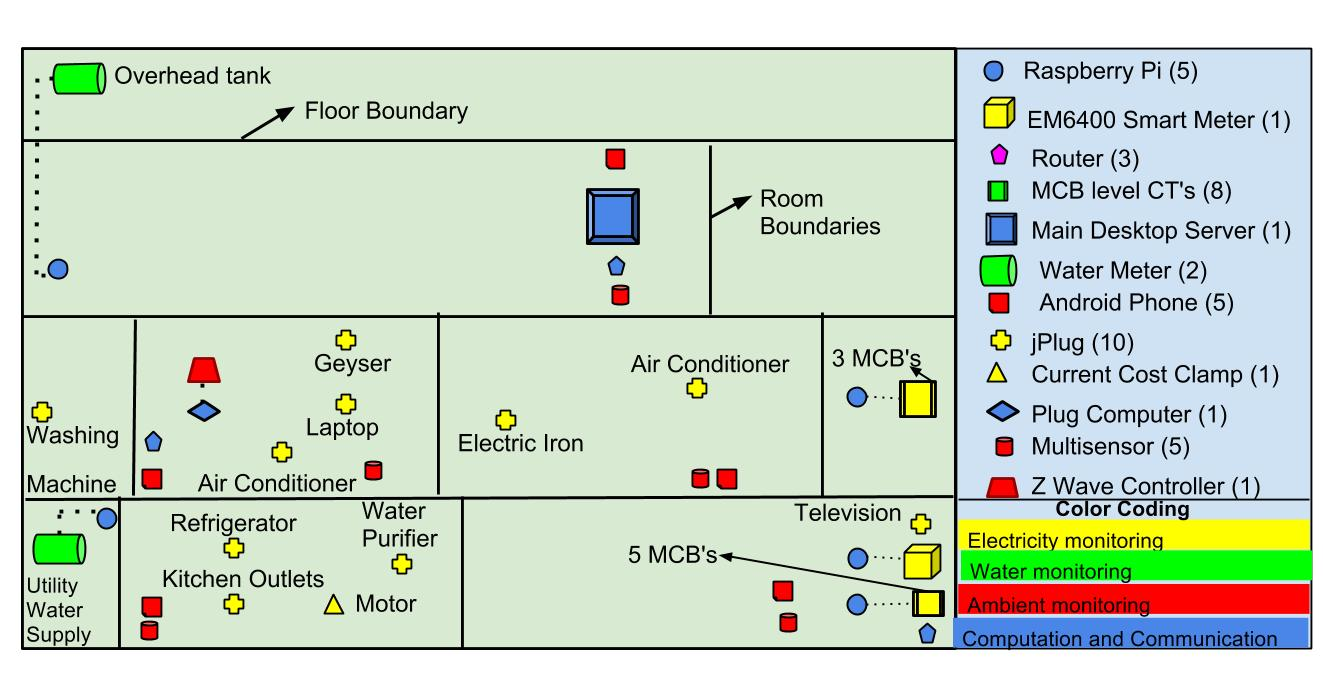
\includegraphics[scale=0.19]{./figures/overall_deployment.jpg}
    \vspace{-10mm}    
    \caption{Schematic showing overall home deployment} 
    \vspace{-2mm}  
    \label{fig:overall}
\end{figure}

\subsection{Sensing Infrastructure}
\label{sec:sensing}
For sensing, we took a ``leave no stone unturned'' approach, where  we chose to monitor as many physical parameters (ambient conditions, electricity usage and water usage) and non-physical parameters (such as network strength and network connectivity) as possible. We took care to deploy these sensors in a way that residents can continue their daily routines without added inconvenience. Constrained by the limited options available in the Indian context, our sensors constitute COTS (procured from both within and outside India) and custom built hardware. %Detailed description of the sensors used for monitoring various parameters are explained next.

\noindent\textbf{Electricity monitoring:} %A typical home electricity setup involves a meter which is installed by utility companies and measures overall electricity usage. Further electric cabling is divided into various Miniature Circuit Breakers (MCB's) which control separate circuits. Typical installations involve putting a separate MCB for each heavy load (such as air conditioners) and clubbing various lights, fans and other smaller loads into separate MCB's. Further each individual appliance is controlled via a switch. There are two types of appliances- i) plug loads like refrigerator and electric iron, which need to be physically ``plugged" into the sockets; ii) loads like lights and fans, which do not need to be ``plugged" in by the user and can directly be switched on or off. We highlight the above described home electricity distribution in \figref{fig:electricity_distribution}. 
Motivated by prior electricity consumption deployments, we also chose to monitor electricity consumption across different granularity- electricity meter monitoring the consumption at the home aggregate level, current transformers (CTs) monitoring current for miniature circuit breakers (MCBs) (each connected to a combination of appliances) and plug level monitors for monitoring plug load based appliance (see \figref{fig:electricity_distribution} for illustration). 
\begin{figure*}[t!] 
    \vspace{-11mm}
    \subfloat[\scriptsize EM6400 Smart Meter]{
    \label{fig:em6400}
    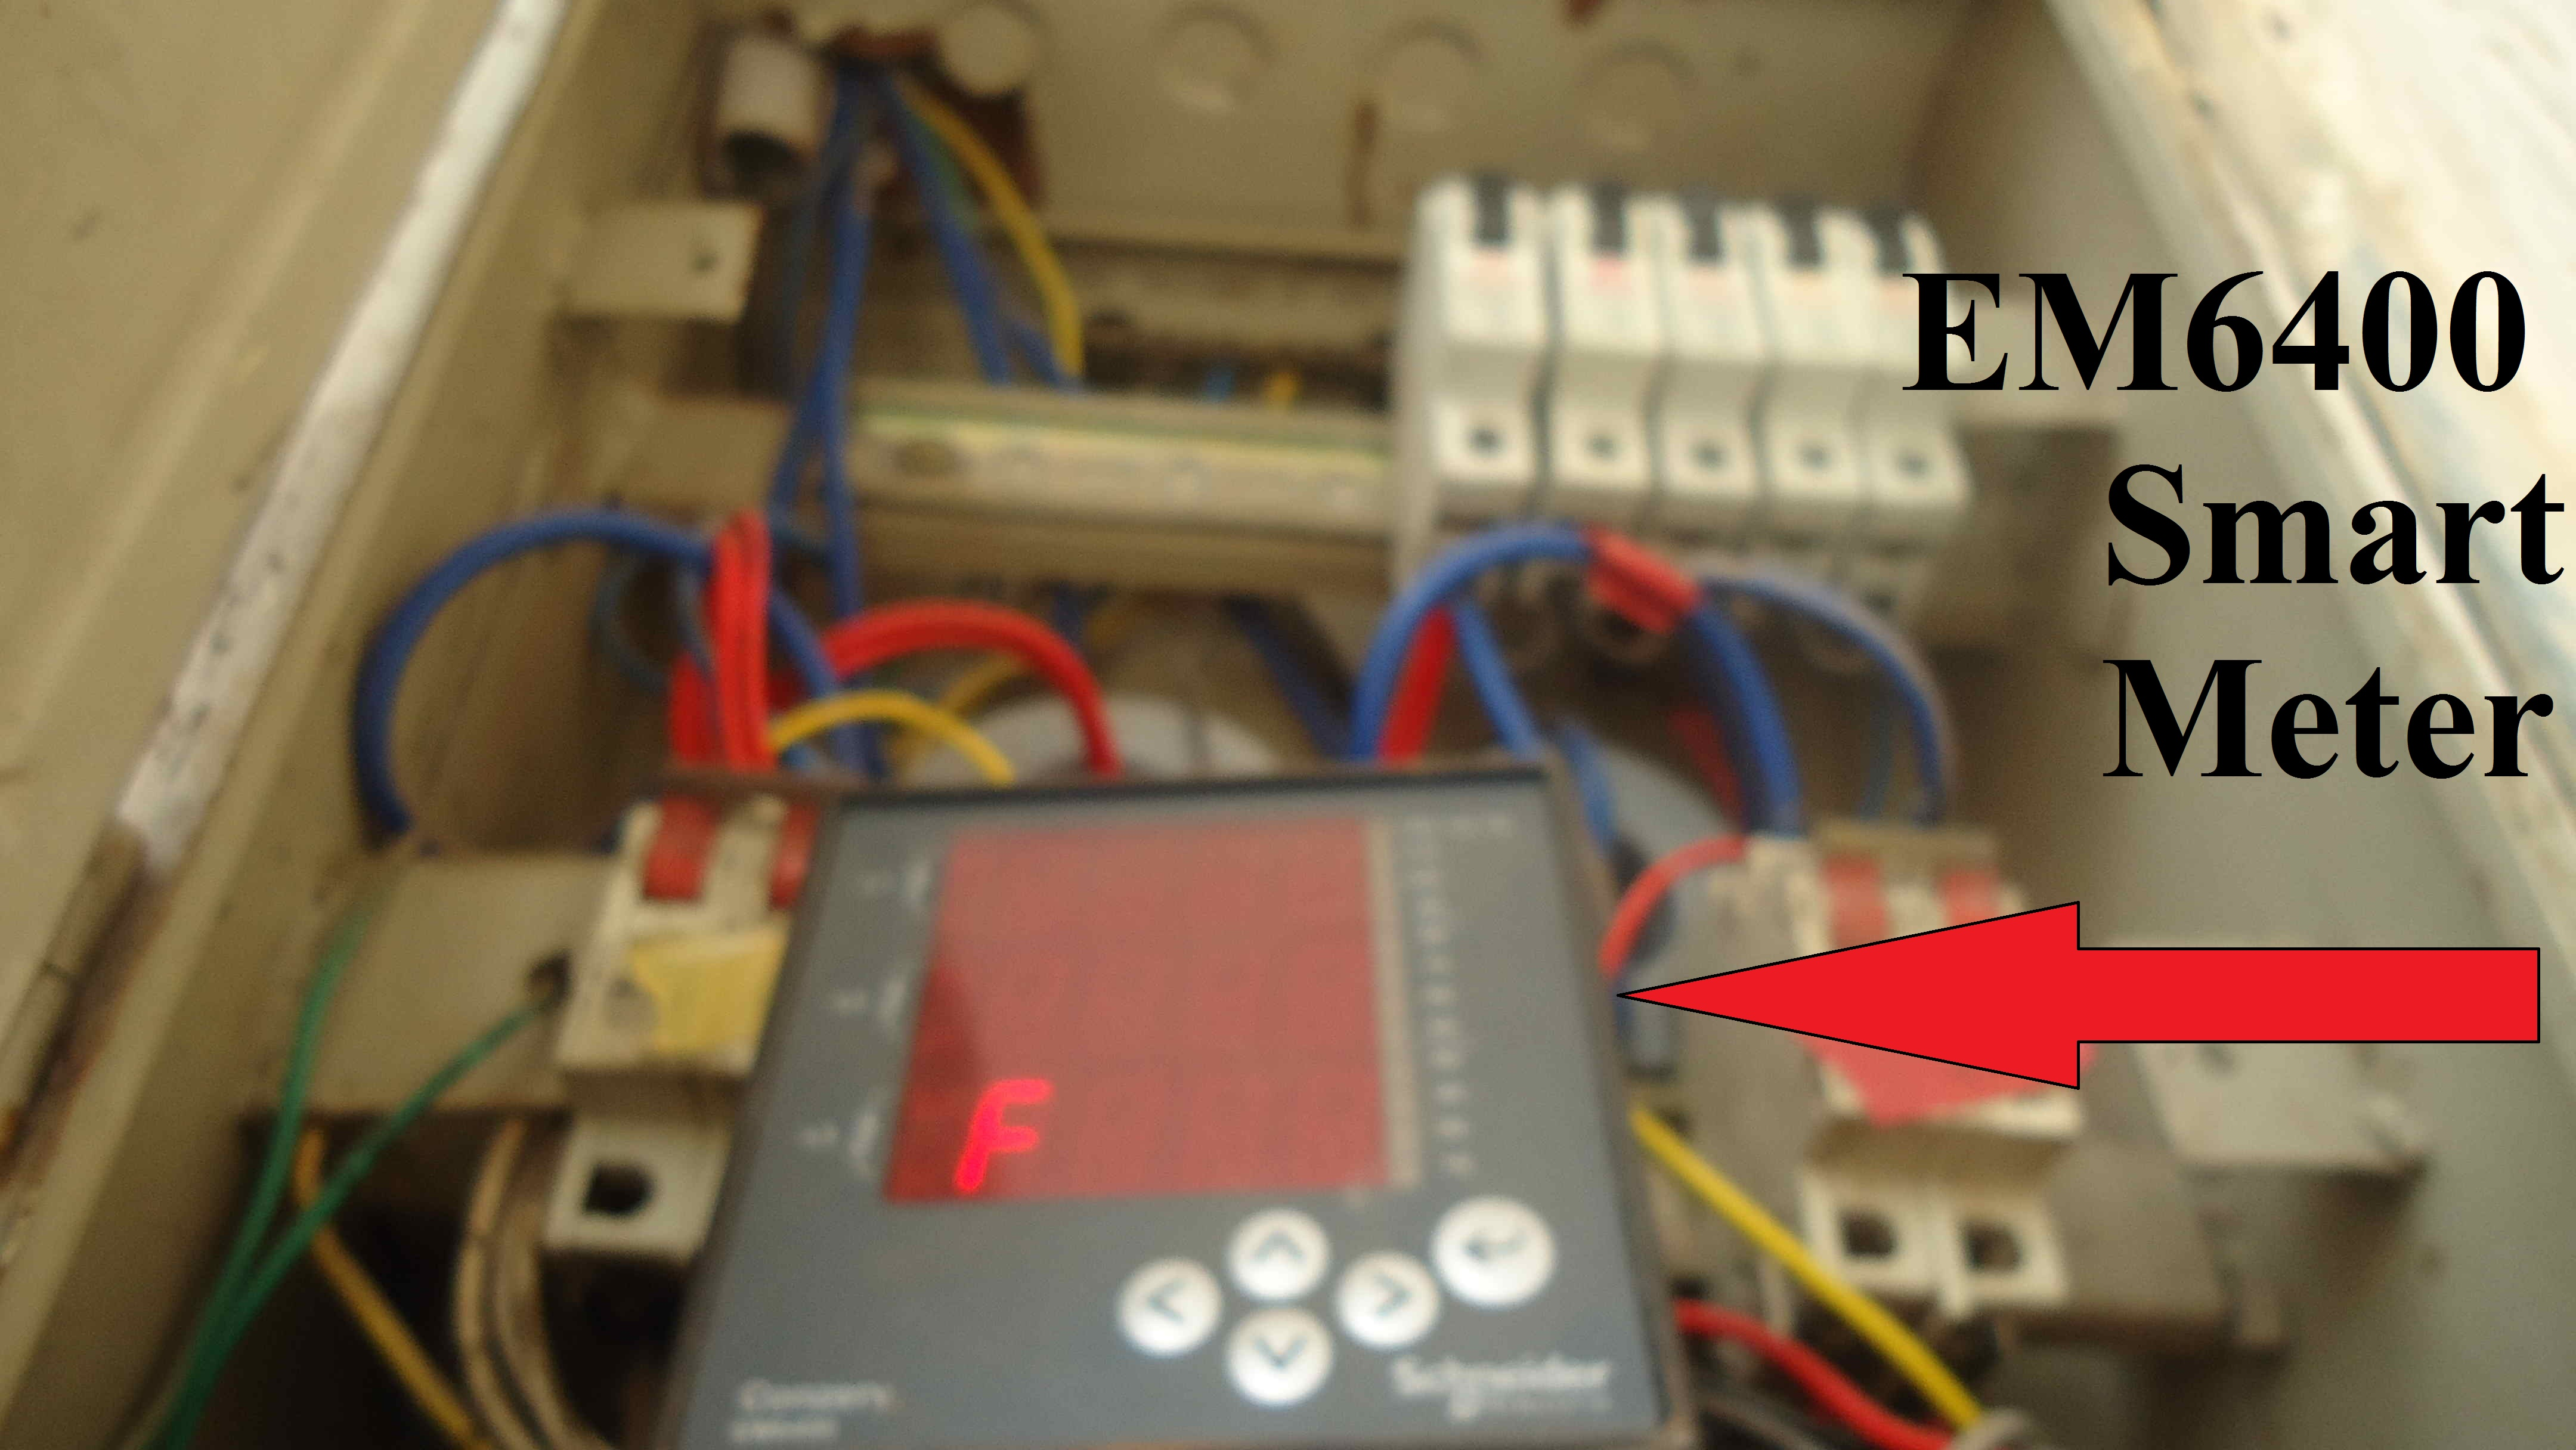
\includegraphics[scale=0.027]{./figures/electric_meter_1.jpg}}
    \hspace{1mm}
     \subfloat[\scriptsize In-house developed CT monitoring system for measuring current from MCBs]{
        \label{fig:ct}
        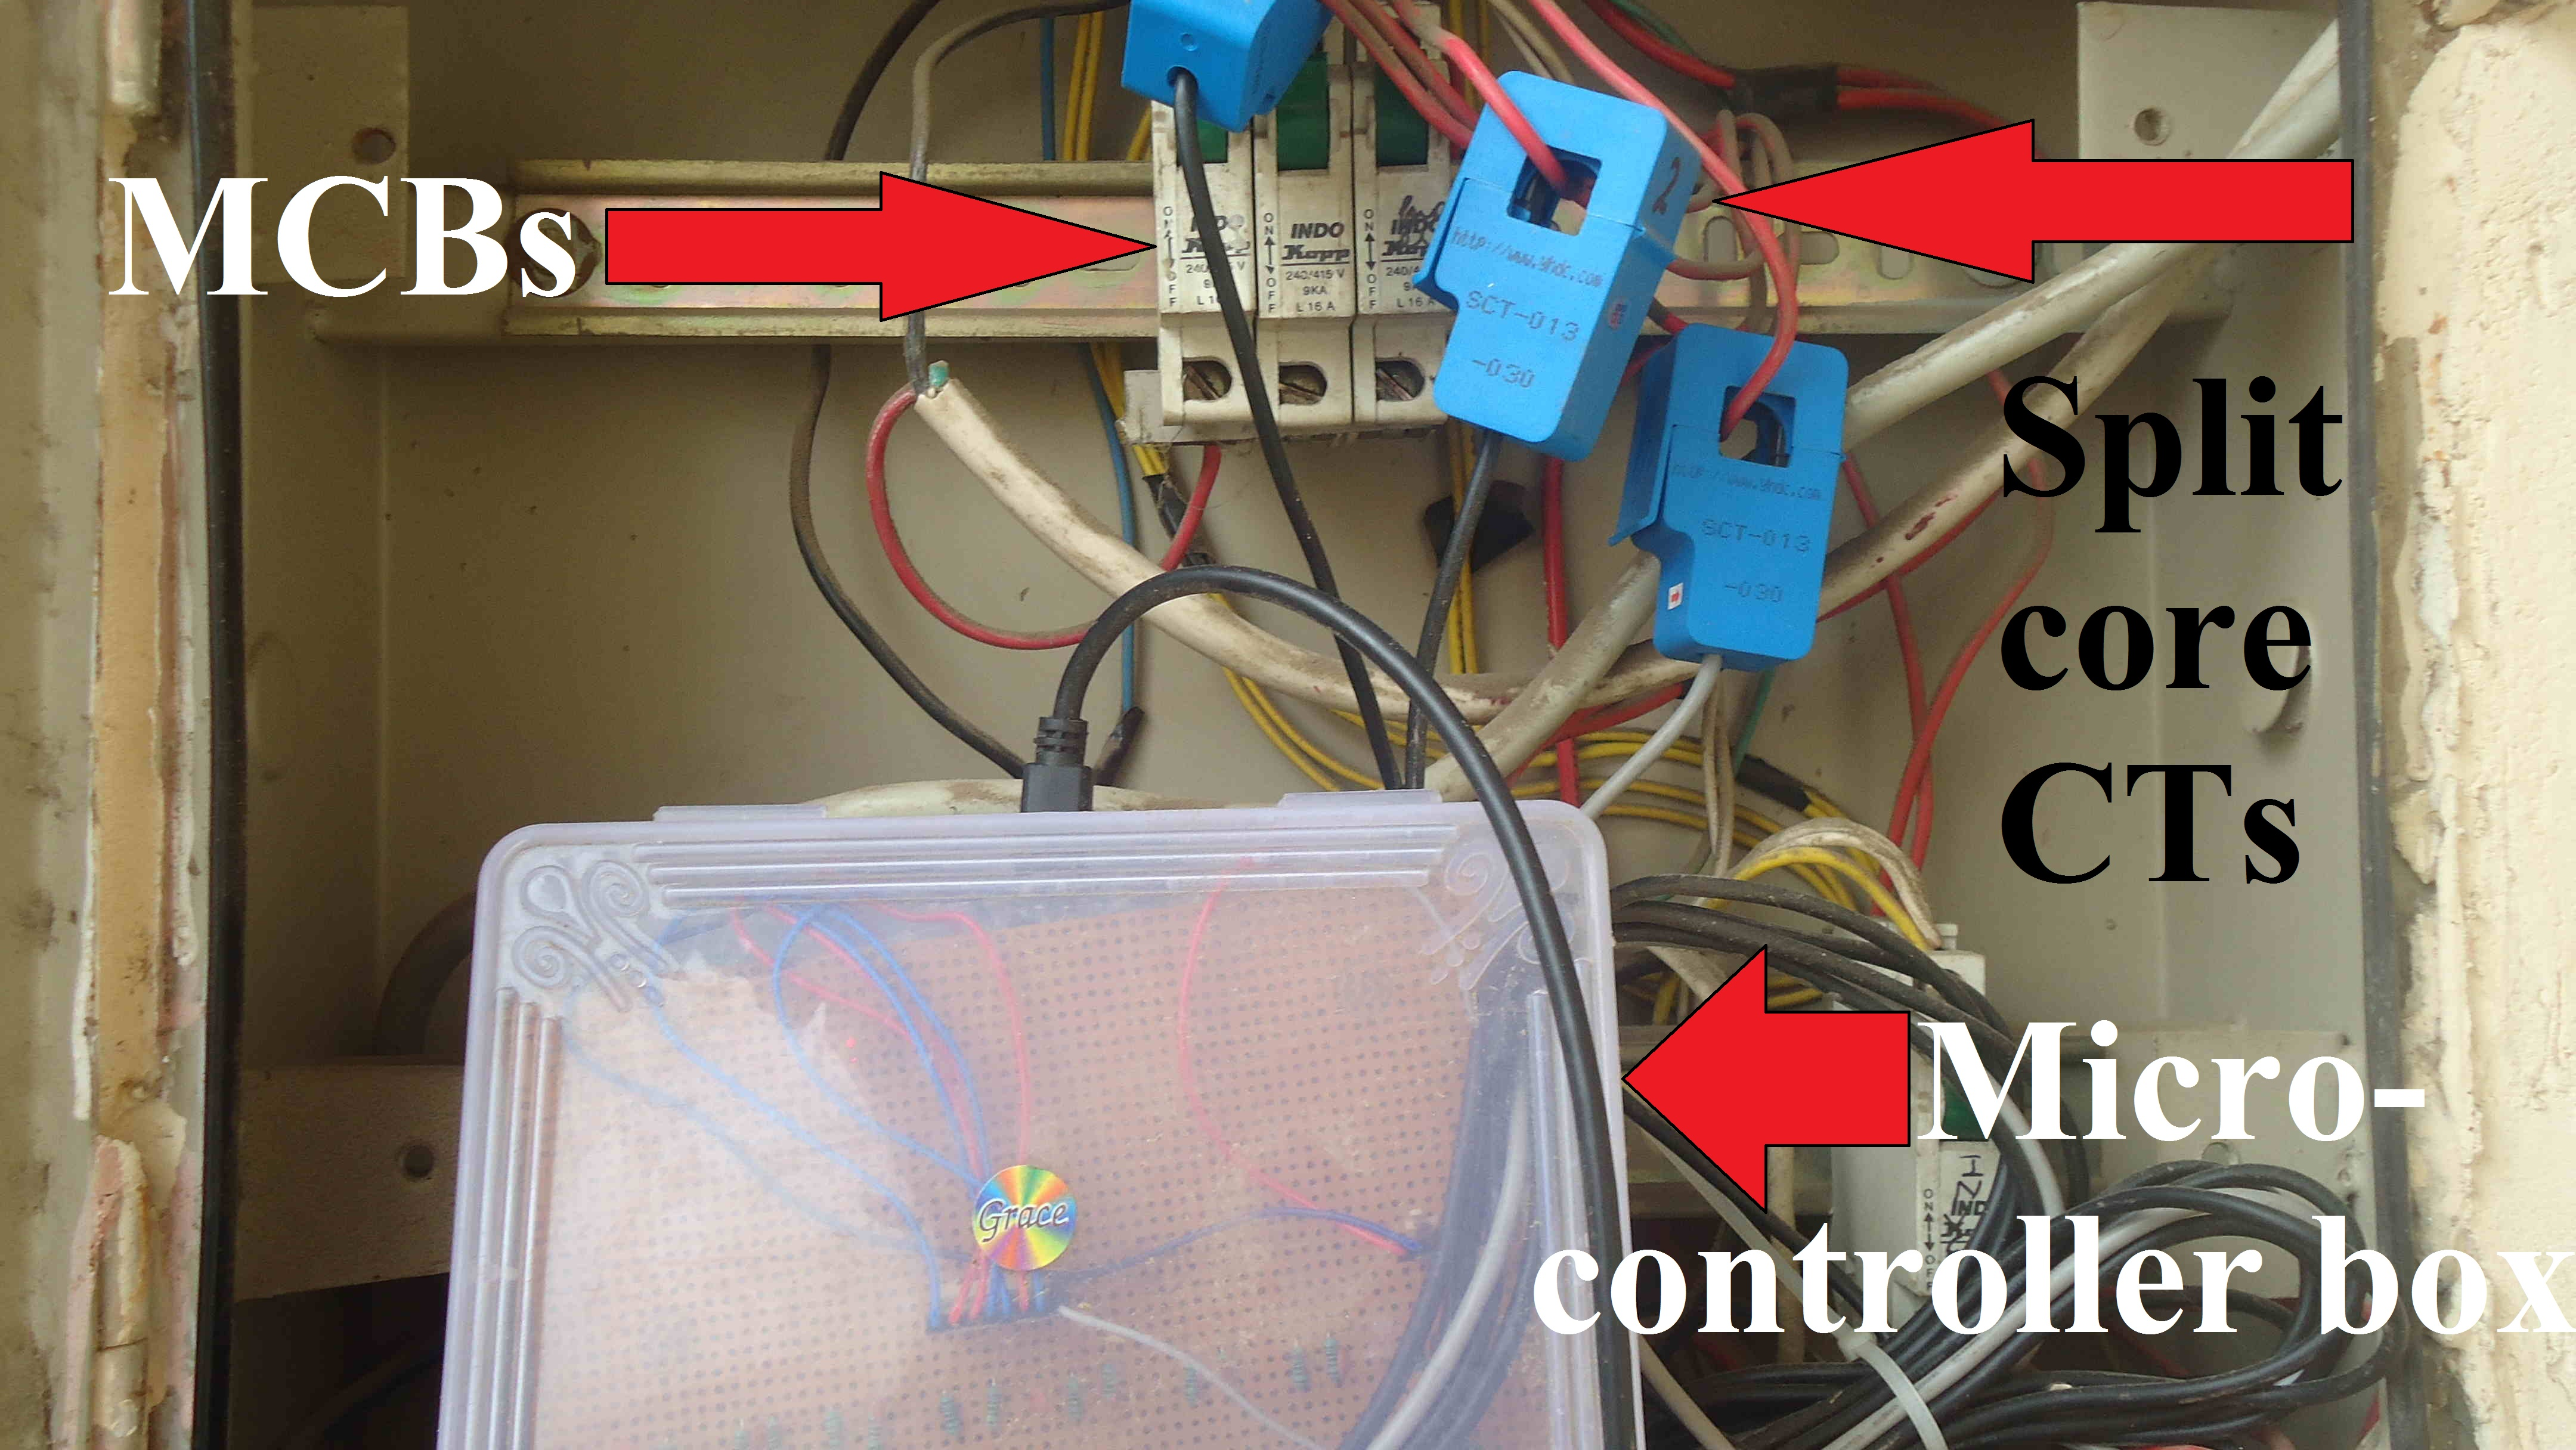
\includegraphics[scale=0.027]{./figures/mcb_2.jpg}}
       \hspace{1mm}
     \subfloat[\scriptsize Appliance level monitoring using jPlug]{
             \label{fig:jplug}
             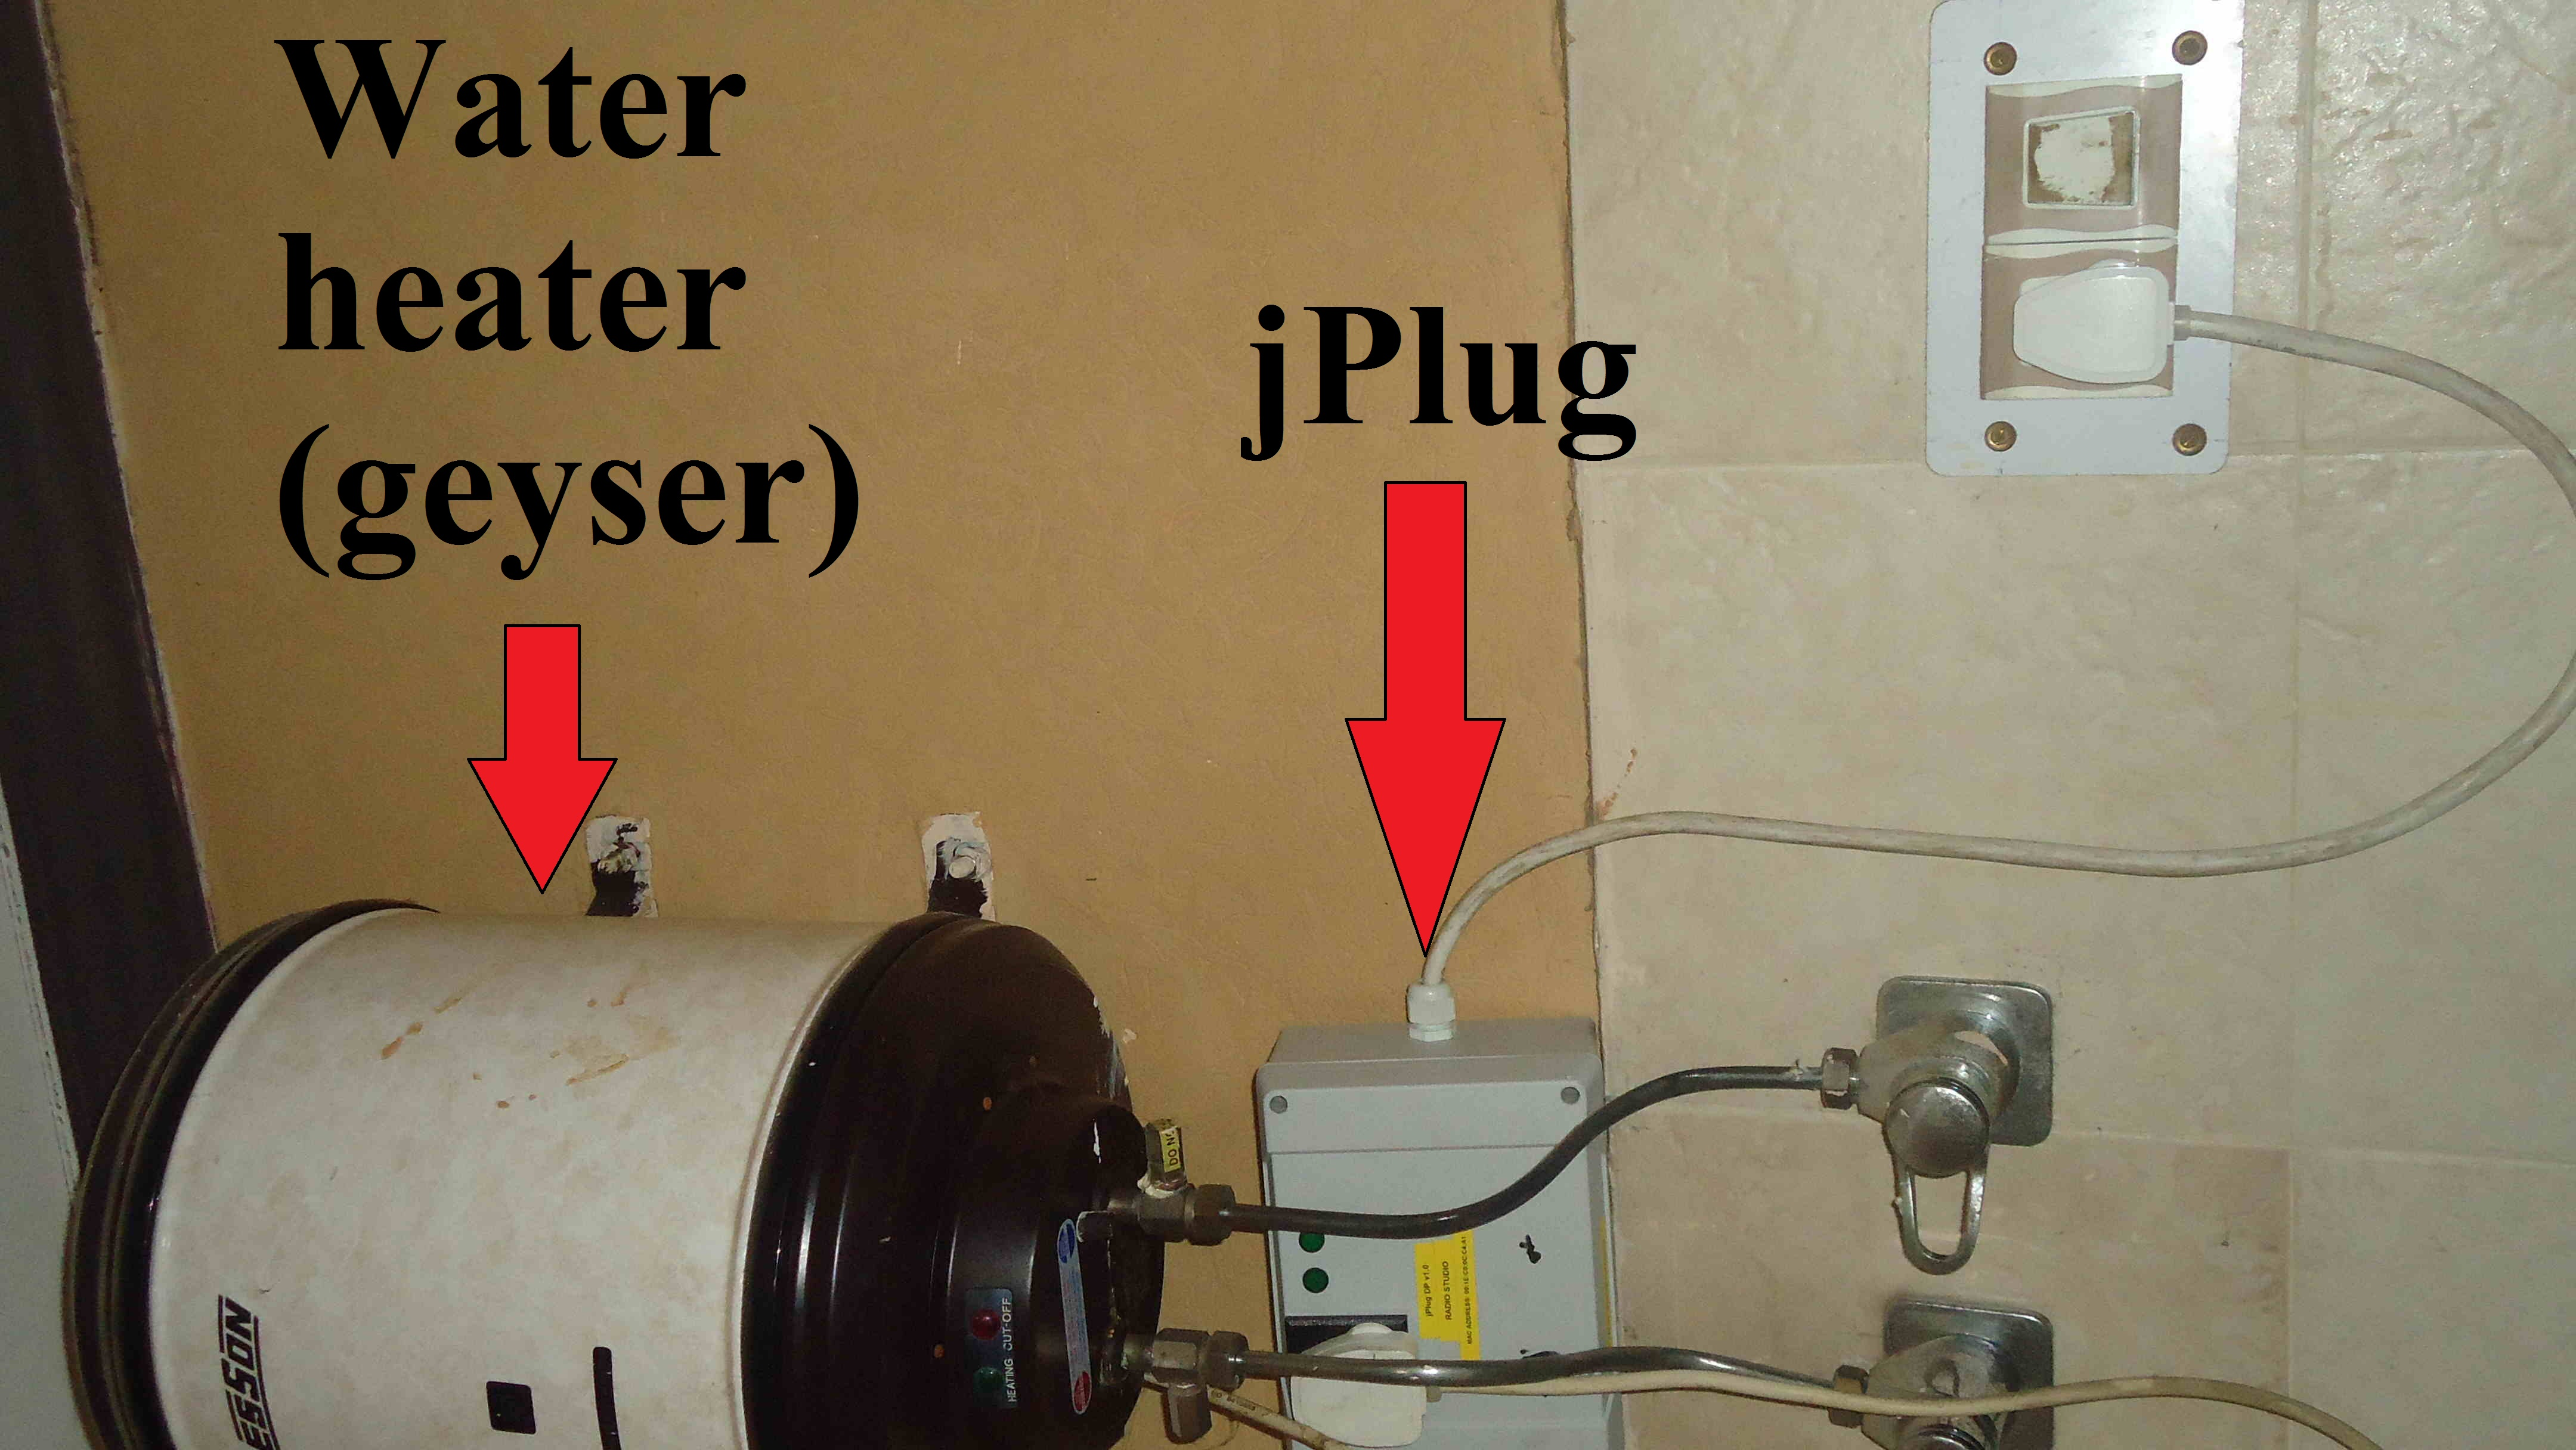
\includegraphics[scale=0.027]{./figures/jplug_2.jpg}}
             \hspace{1mm}
          \subfloat[\scriptsize Appliance level monitoring using Current Cost CT]{
                  \label{fig:cc}
                  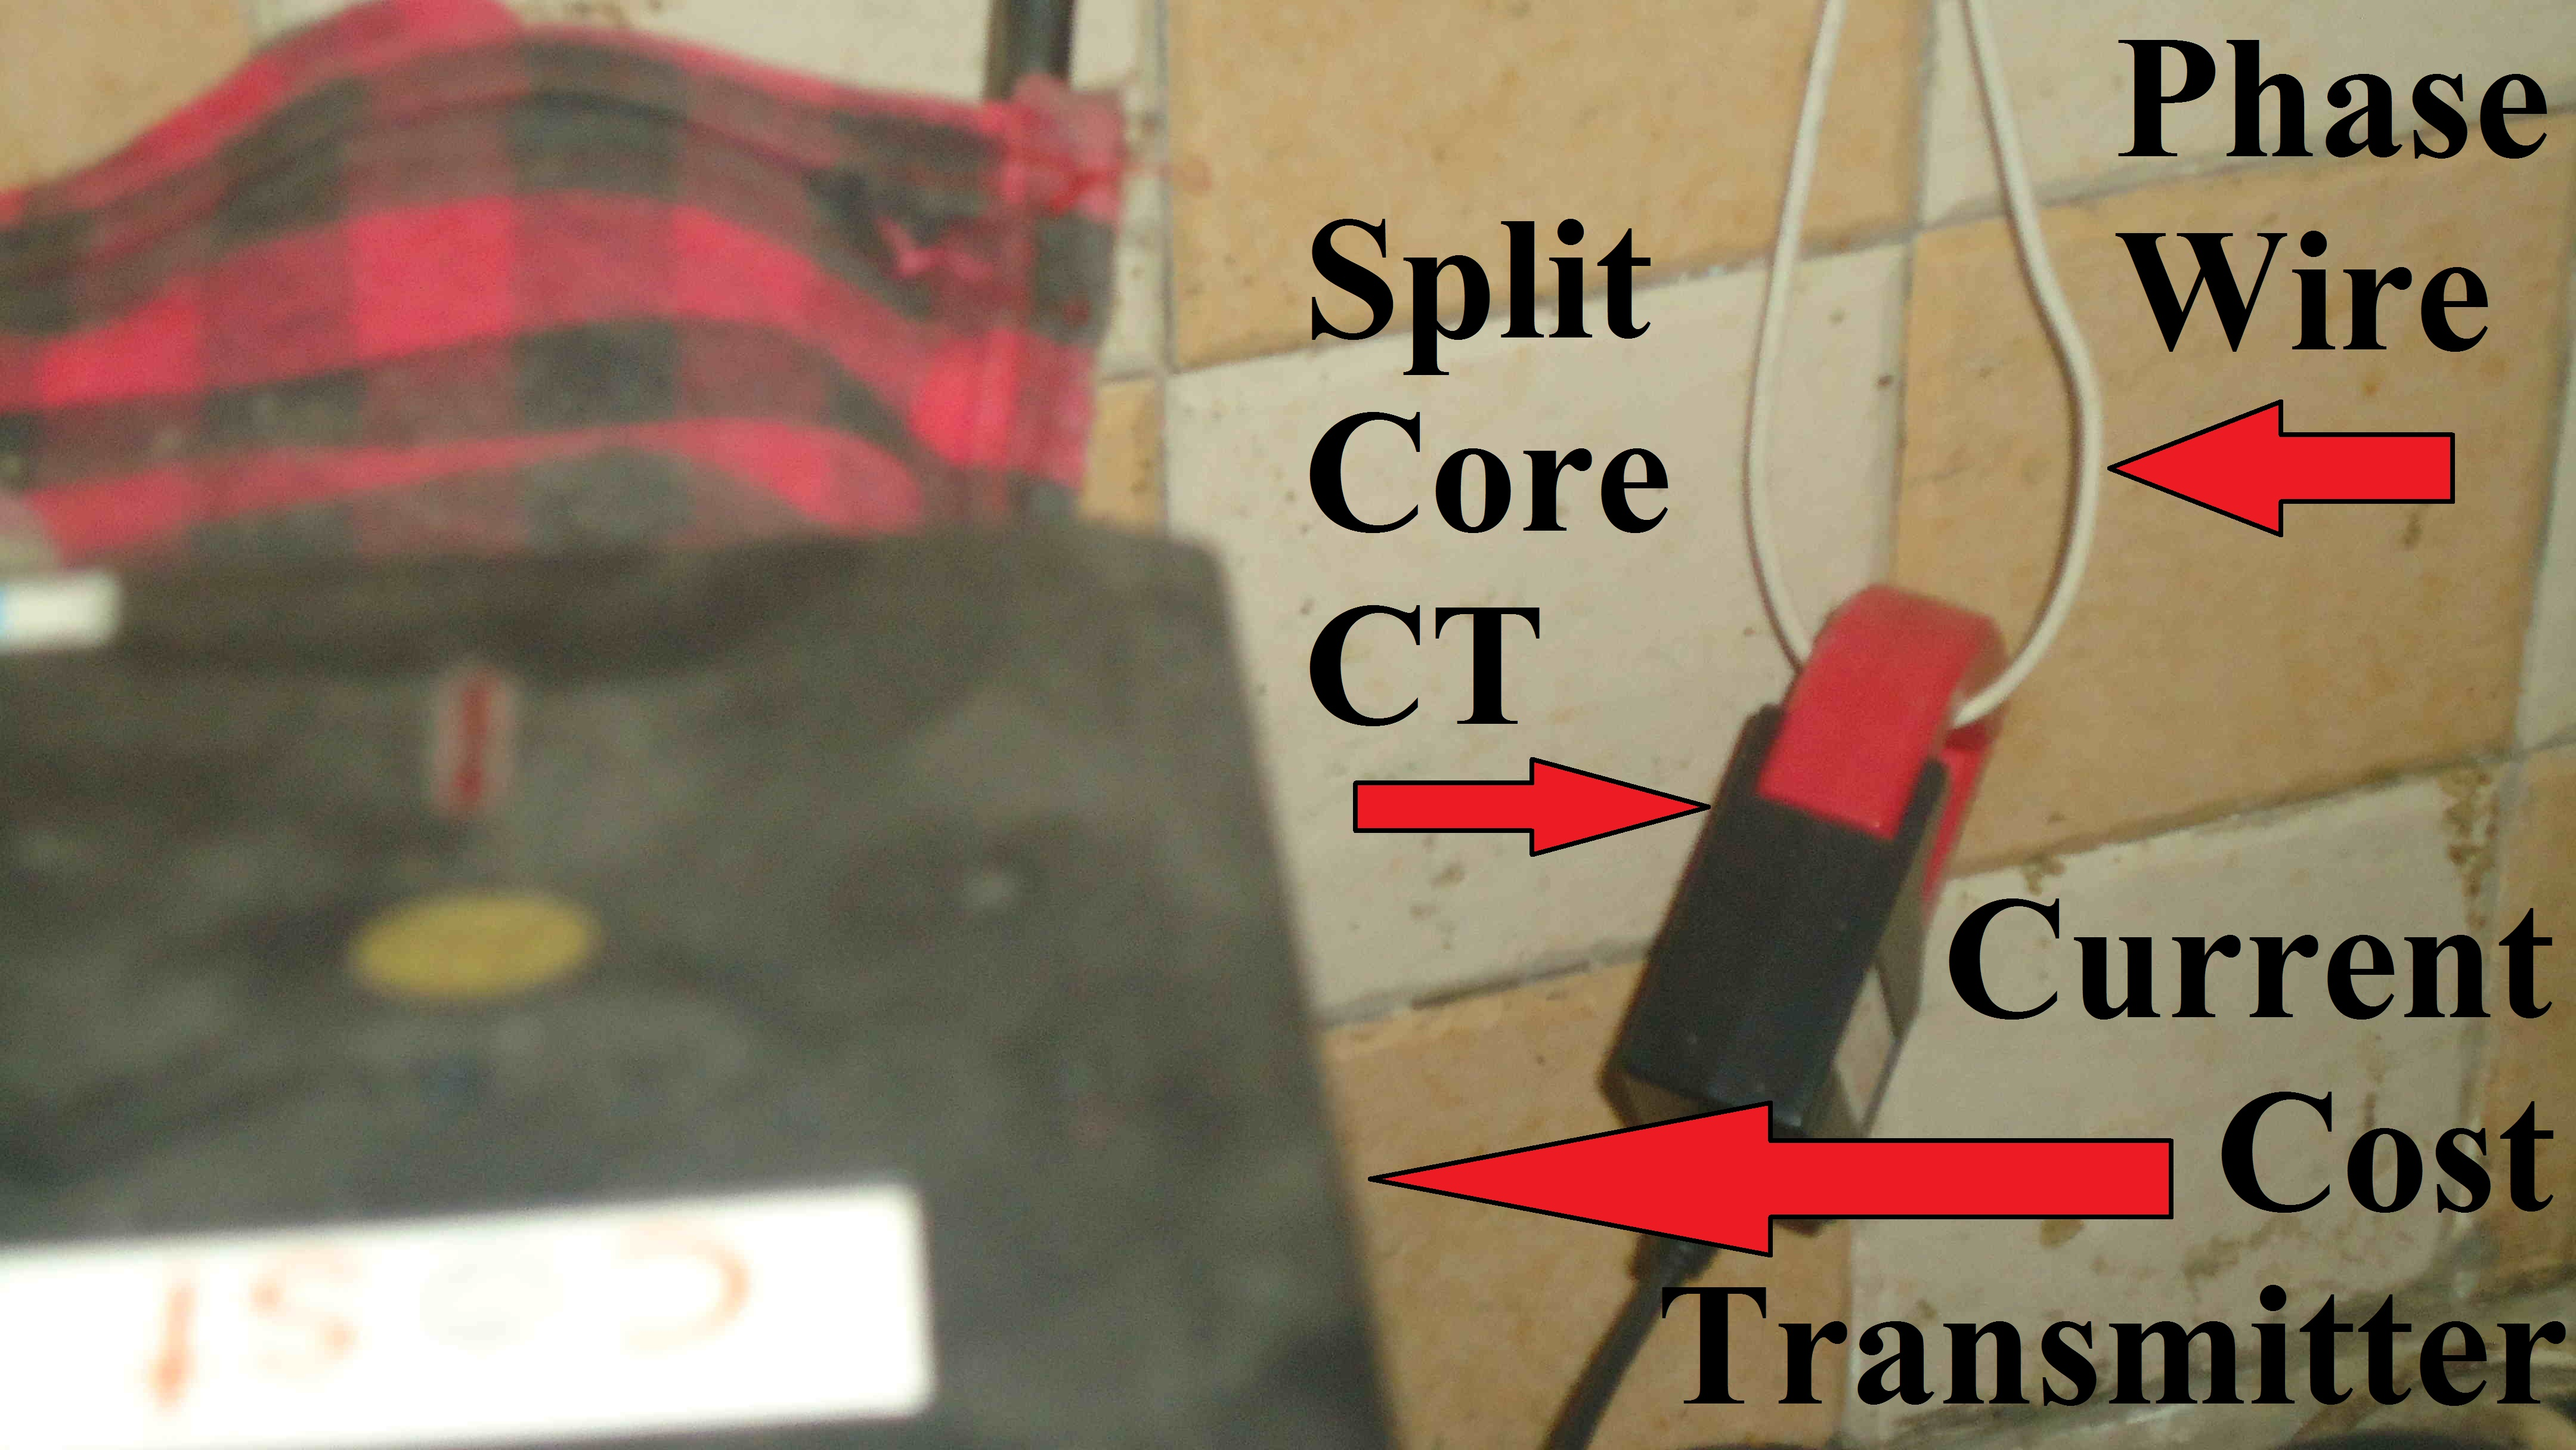
\includegraphics[scale=0.027]{./figures/cc_1.jpg}}
    %\hspace{0.02\columnwidth}
    \newline
    \vspace{-2mm}
    \subfloat[\scriptsize Water Meter]{
    \label{fig:water_meter}
        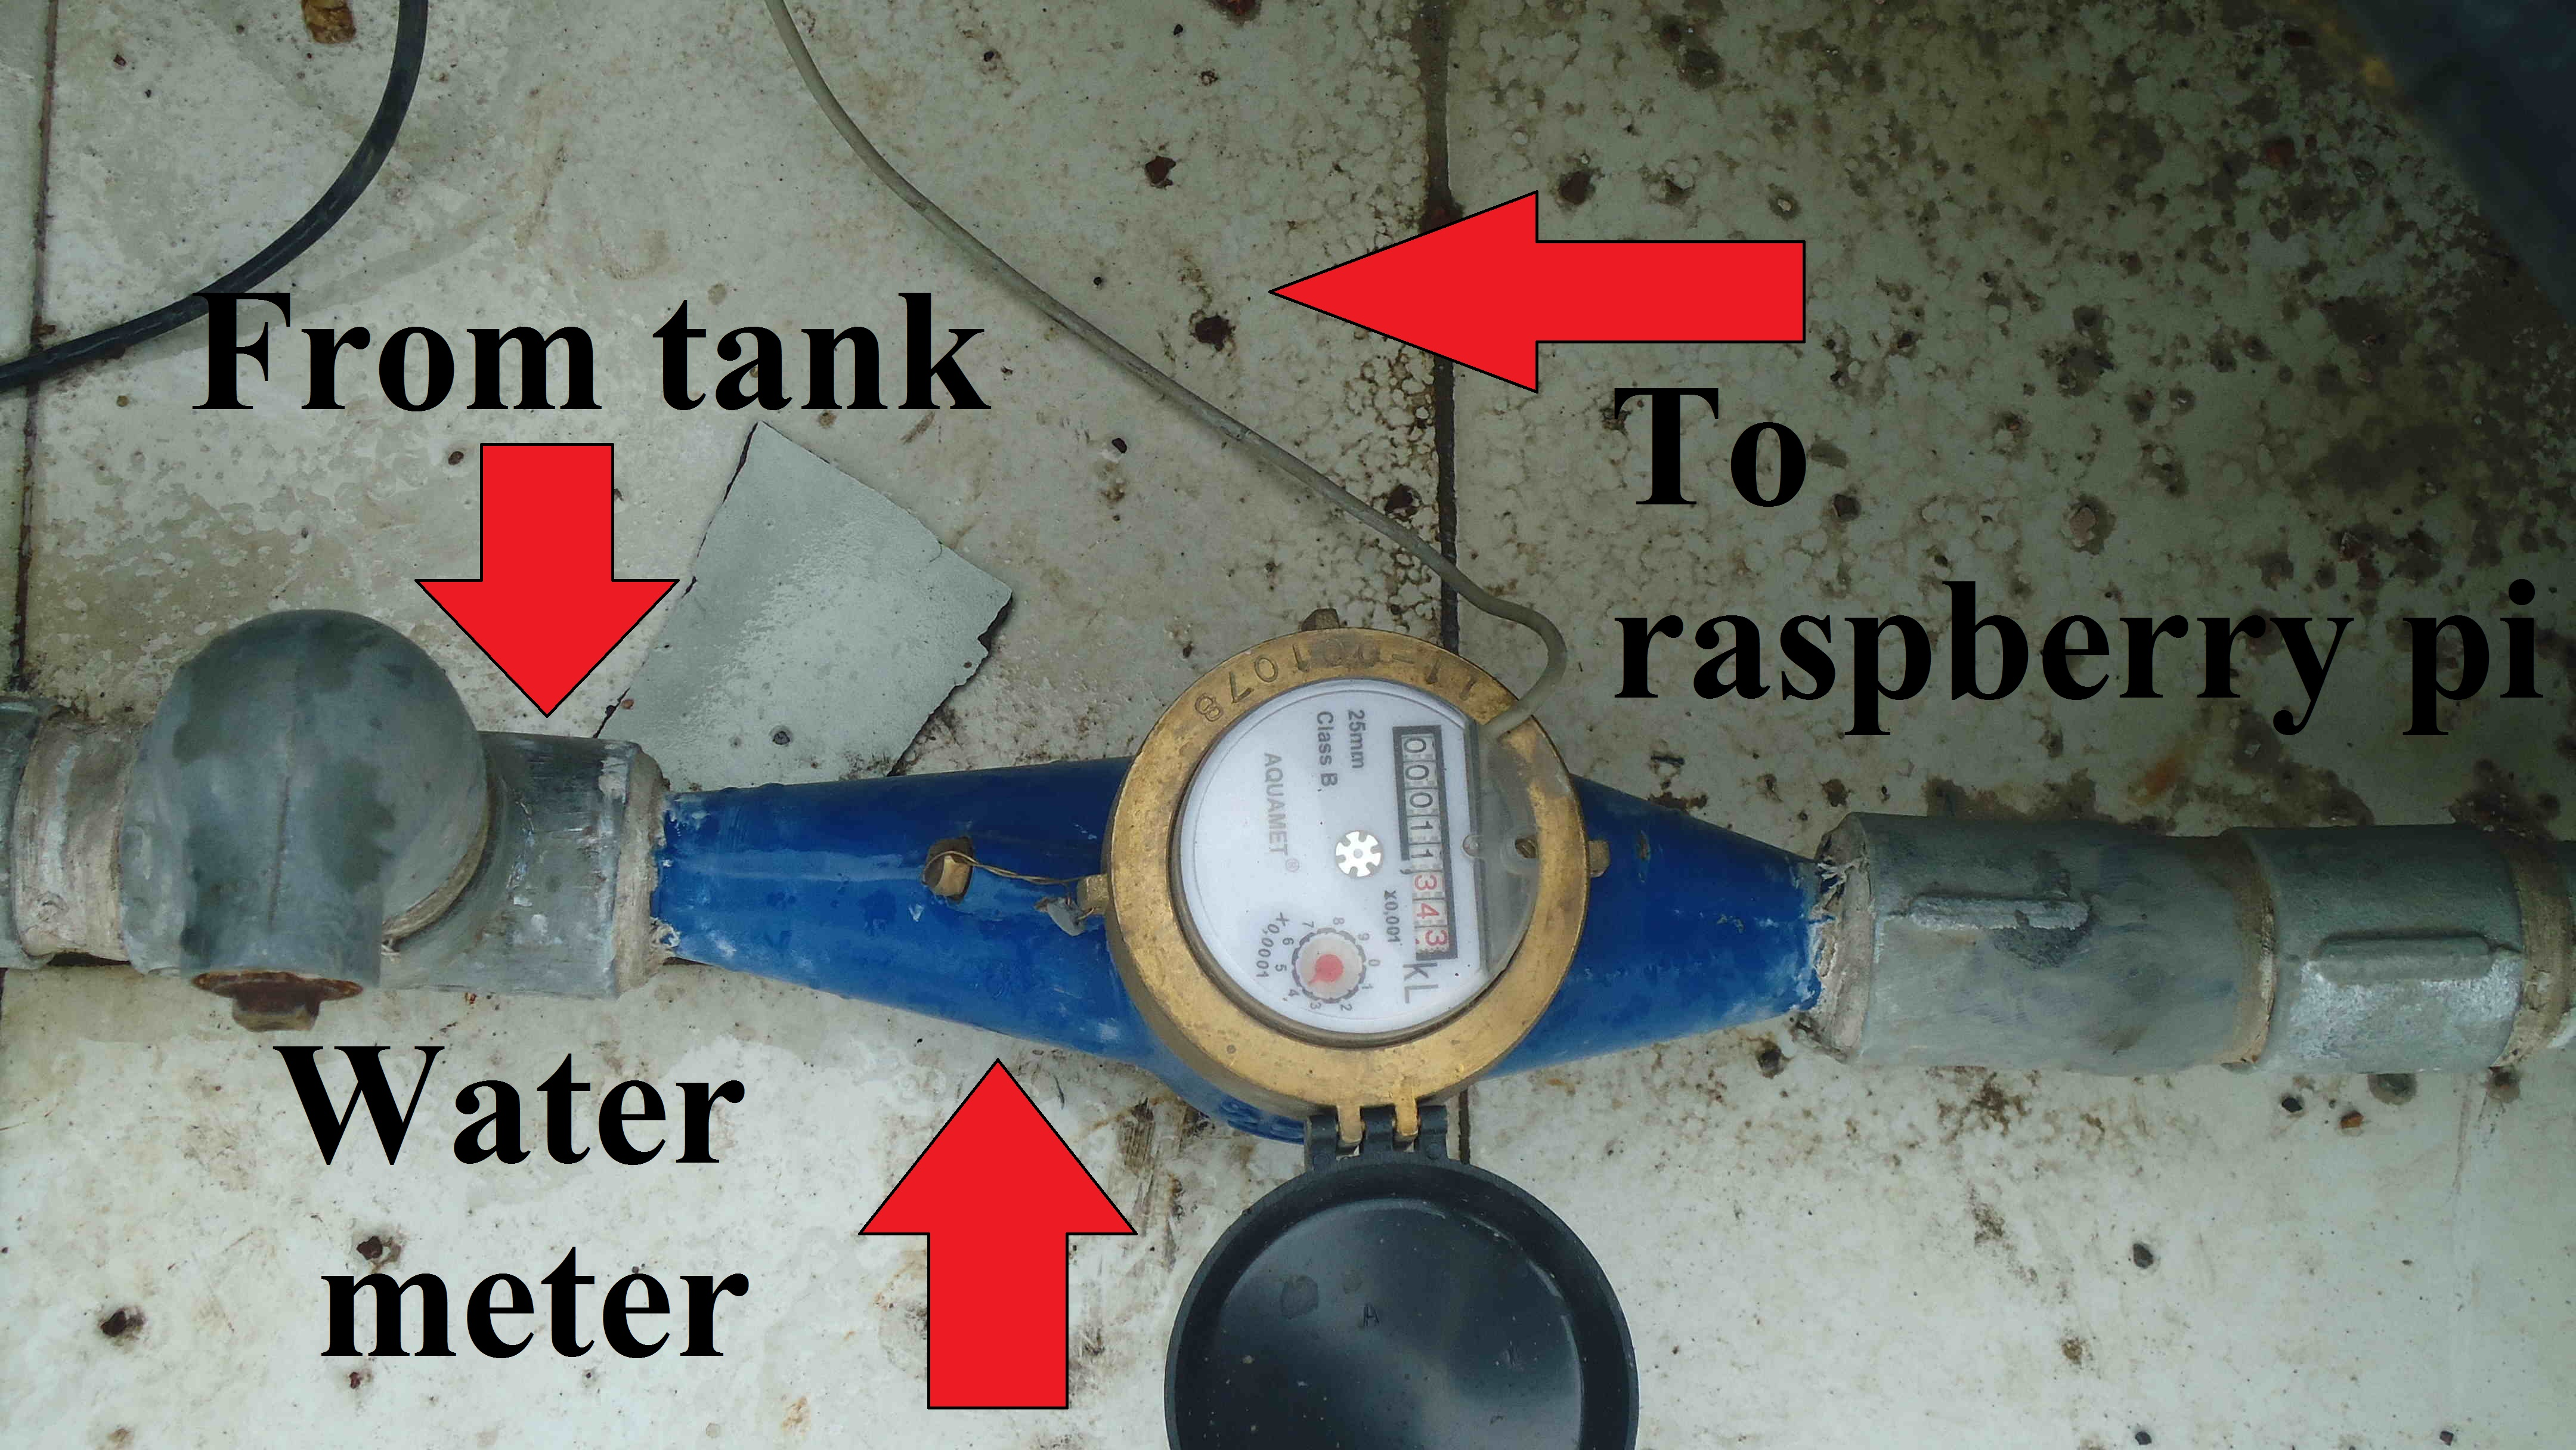
\includegraphics[scale=0.027]{./figures/water_meter_2.jpg}}
        \hspace{1mm}
        \subfloat[\scriptsize RPi collecting water meter data using GPIO pins]{
                             \label{fig:rpi}
                                 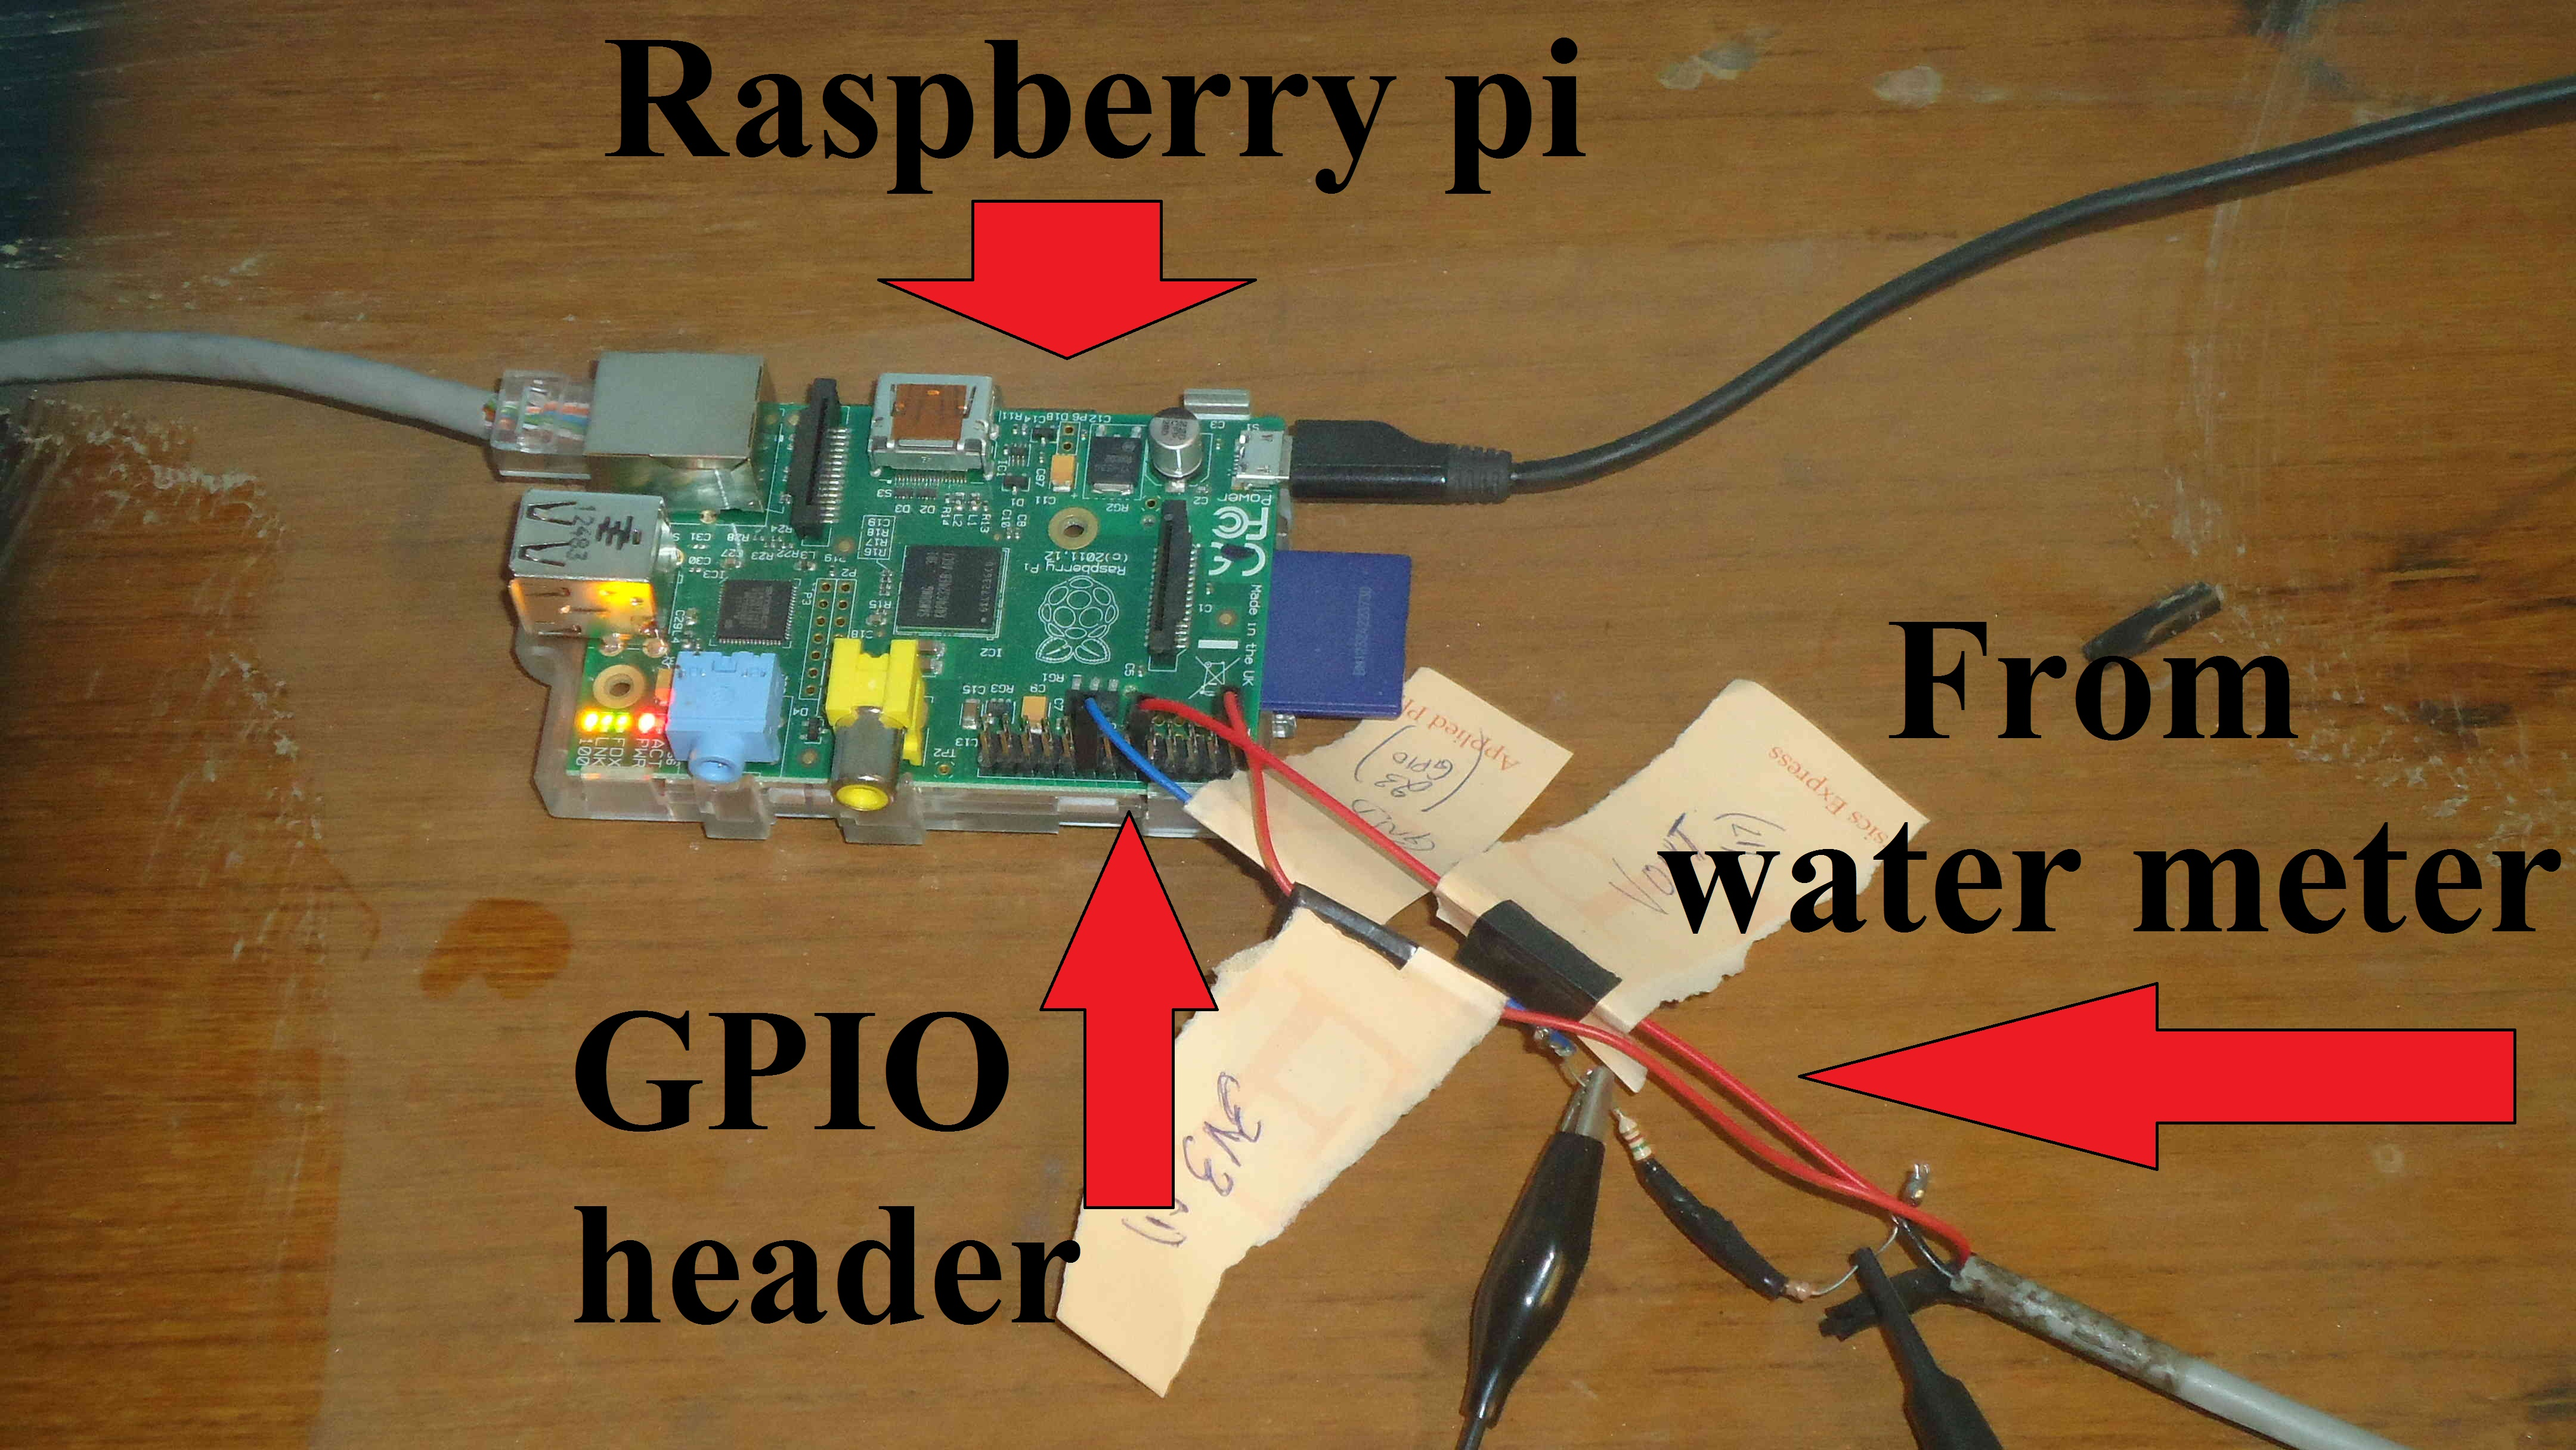
\includegraphics[scale=0.027]{./figures/rpi_2.jpg}}
                                  \hspace{1mm}
     \subfloat[\scriptsize Android phone and Express Control ZWave multisensor used to measure ambient parameters]{
        \label{fig:ambient}
            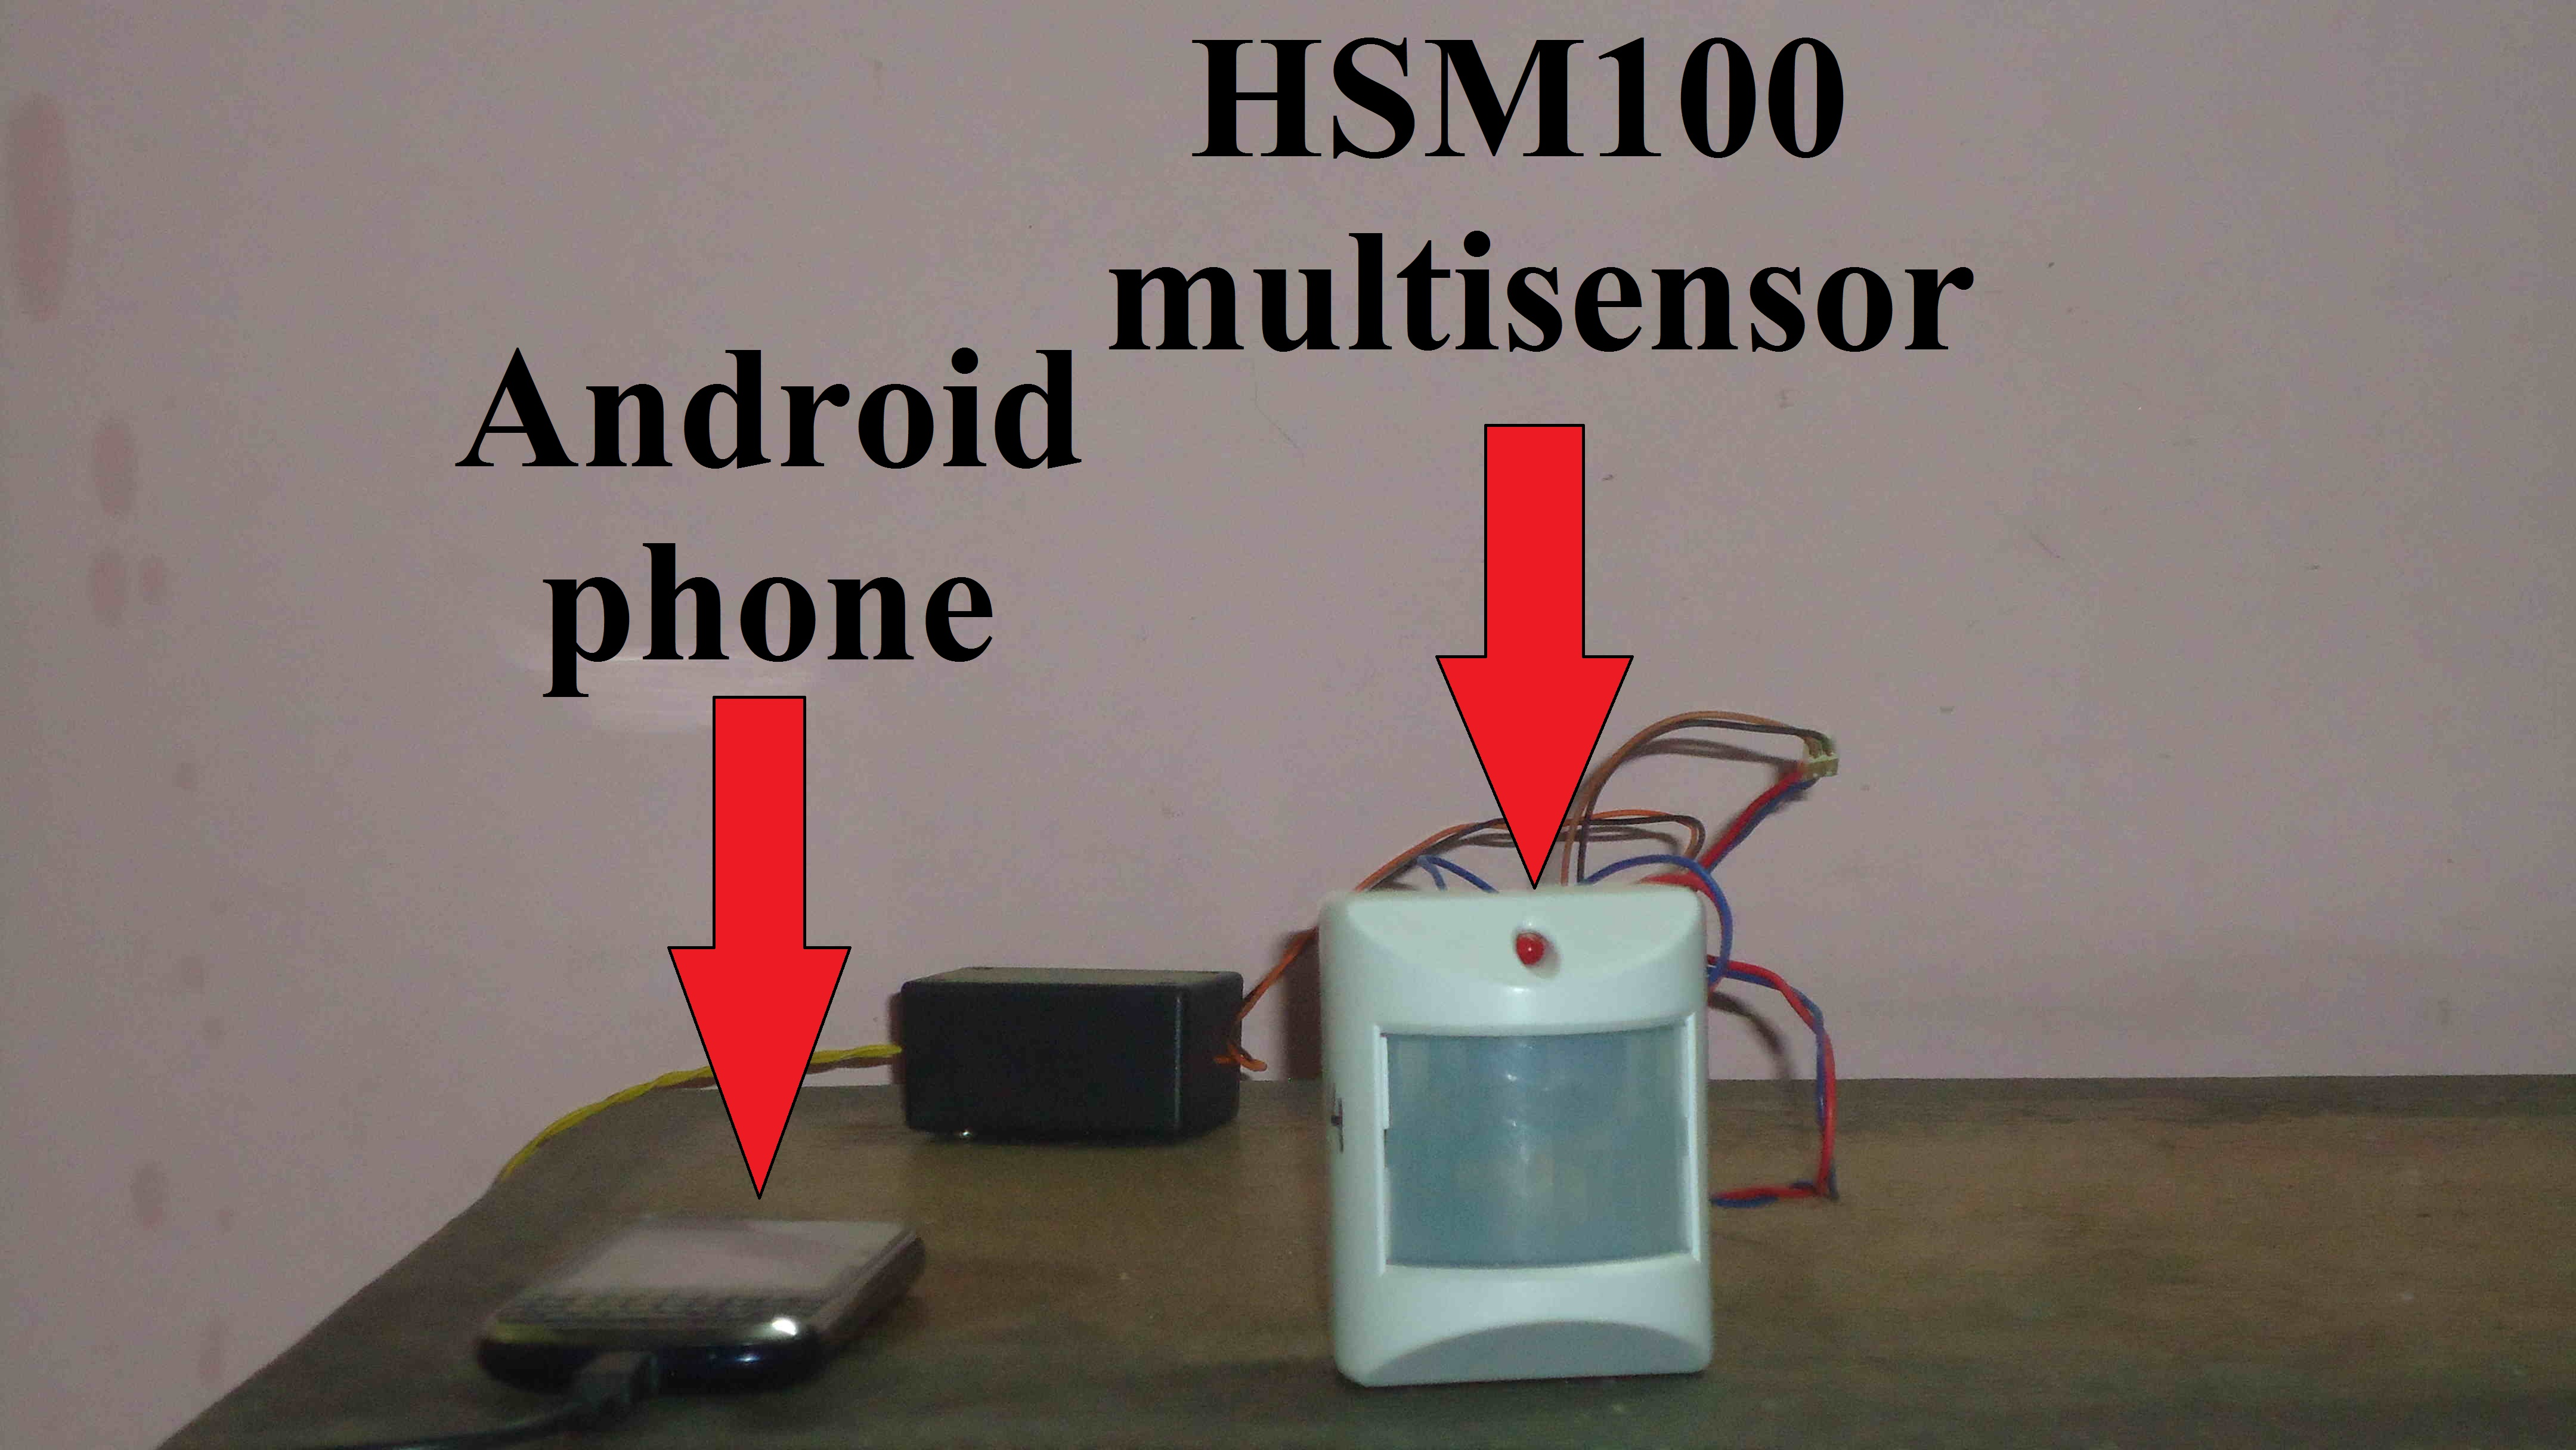
\includegraphics[scale=0.027]{./figures/ambient_2.jpg}}
            \hspace{1mm}
       \subfloat[\scriptsize Plug computer collecting data from ZWave controller and connected to the router via an Ethernet cable]{
              \label{fig:plug}
                  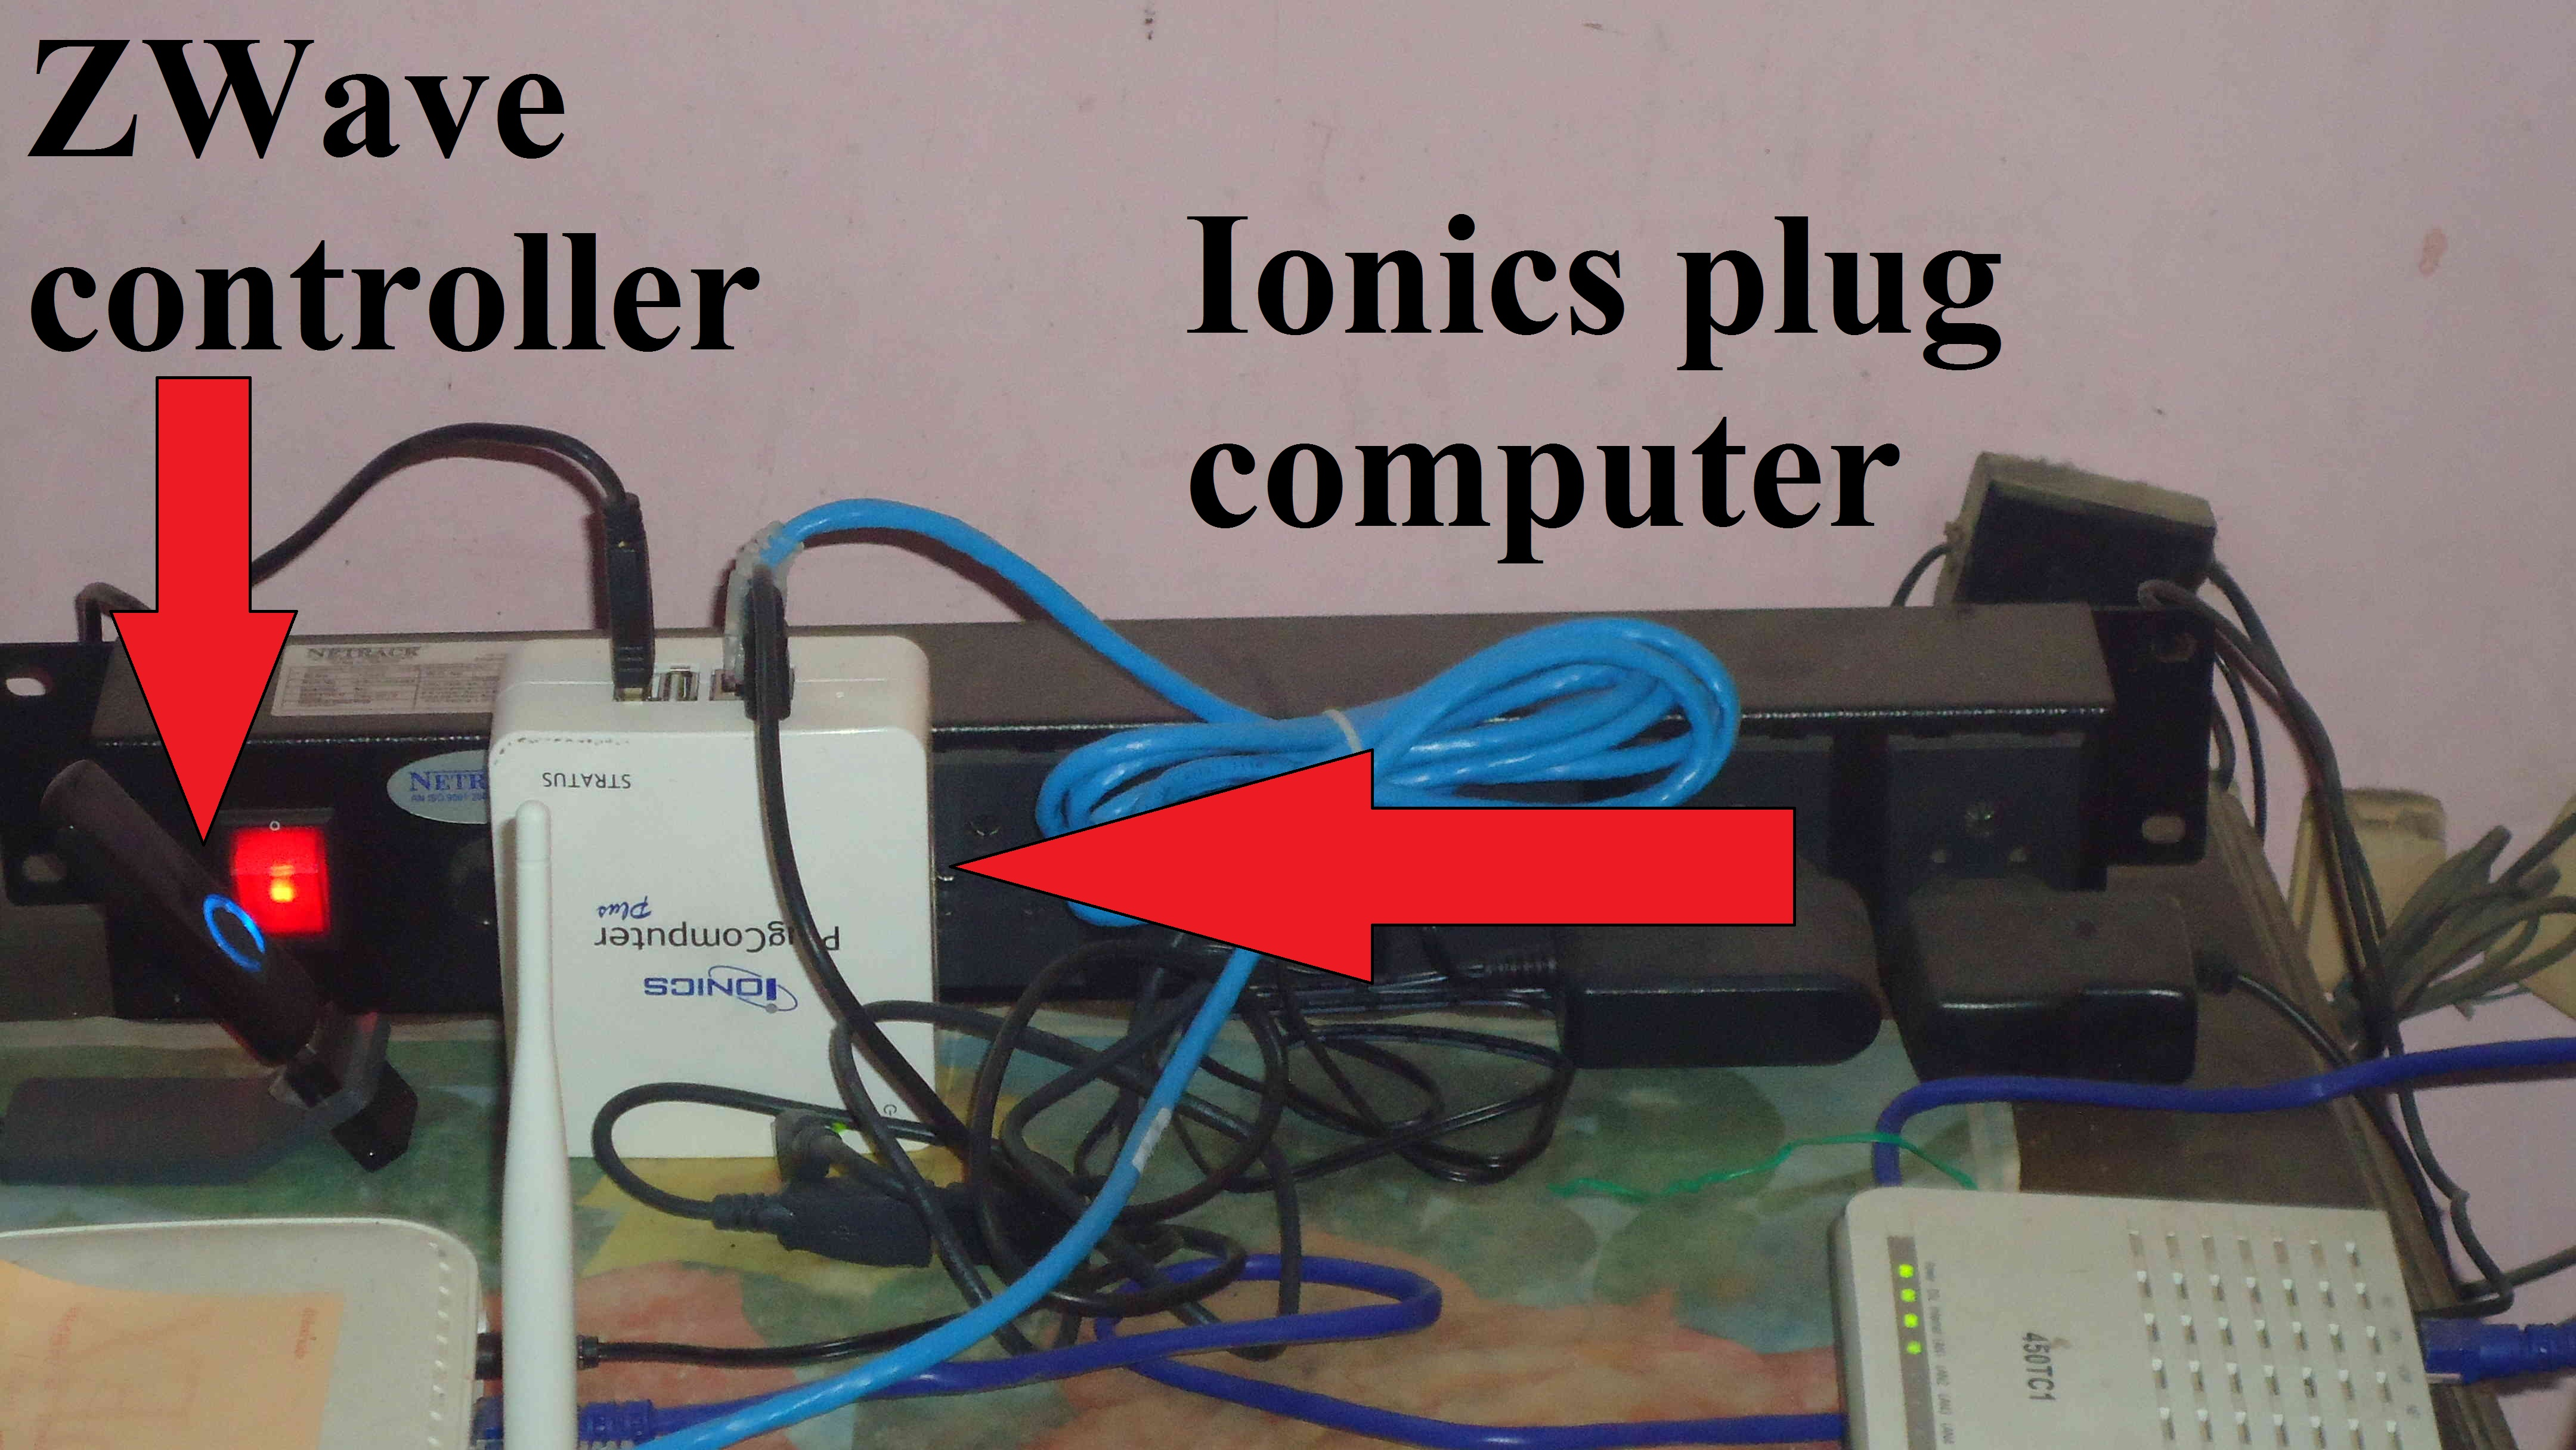
\includegraphics[scale=0.027]{./figures/plug_2.jpg}}
                 
         
	\vspace{-1mm}
    \caption{Sensing, computation and communication equipment used for deployment}

    \label{fig:deployment}

\end{figure*}

\begin{enumerate}[leftmargin=1em]\denselistbib
\vspace{-1.5mm}\item \textbf{Meter level:} Schneider Electric EM6400\footnote{\url{www.goo.gl/01edPS}} smart meter is used to instrument the main power supply (see \figref{fig:em6400}).% showing EM6400 smart meter deployed in the electricity panel). %While cheaper variants from the same company were available, we chose to use EM6400 as it also provides reactive power. This additional information has been known to be useful for NILM applications~\cite{hart}. 
%~A 30:5 ratio CT was used on the power mains coming from the grid to ensure that the load current is transformed within the permissible limits (5 A) of the meter. 
~Necessary parameters including voltage, current, frequency, phase and power were read at 1 Hz using Modbus over RS485-serial link provided by EM6400. 
%A robust deployment was easily undertaken by a paid electrician thus demonstrating that the support required for large scale smart metering deployments exists in the Indian context. 

\vspace{-1.5mm} \item \textbf{Circuit level:} Split-core CTs, clamped to individual MCBs, are used for monitoring circuit level current. Since no commercial solution was easily available in India for panel level monitoring, we used a low cost microcontroller platform to measure current output from CTs and communicate it's RMS value over serial UART interface (\figref{fig:ct} illustrates CTs monitoring 3 MCBs on the first floor MCB box) to a single board computer. A total of 8 CTs were used to monitor different MCB circuits in the home.
%Since no commercial solution was easily available in India for panel level monitoring, we used a low cost microcontroller platform to measure current output from CTs at 125 KHz, calculate the RMS value and communicate it over serial UART interface (\figref{fig:ct} illustrates CTs monitoring 3 MCBs on the first floor MCB box) to a single board computer. A total of 8 CTs were used to monitor different MCB circuits in the home.

\vspace{-1.5mm} \item \textbf{Appliance level:} Similar to circuit level monitors, there are no good commercial options for plug level monitors in Indian context. Correspondingly, we worked with our collaborators who in-house developed jPlug\footnote{A variant of nPlug~\cite{nplug}} to measure individual appliance power consumption. Ten jPlugs were used to monitor different plug-load based appliances across the home. 
%jPlug sits in between an appliance and the socket and provides multiple parameters (including voltage, current, phase and frequency) at 1 Hz. 
jPlug measures multiple parameters including voltage, current, phase and frequency and uploads them using HTTP POST. We also used Current Cost (CC) based CT to measure the power consumption for electric motor (used to pump water), which is not a plug-load, but has a significant power consumption (approx. 700 Watts). CC exposes apparent power data over the USB port.  jPlug and CC are shown in \figref{fig:jplug} and \figref{fig:cc} respectively.
\end{enumerate}
\begin{table*}[t!]
\footnotesize
\centering
\vspace{-6mm}
\caption{Details of sensing infrastructure used in our deployment}
\vspace{-4mm}
\label{tab:sensing}
\tabcolsep=0.015cm
\begin{center}
\begin{tabular}{|p{1.7cm}|p{2.0cm}|p{3.3cm}|p{1.5cm}|p{1.5cm}|p{2.0cm}|p{5.2cm}|}
\hline
\textbf{Sensor name} & \textbf{Procurement} & \textbf{Sampling frequency} & \textbf{Granularity} & \textbf{Quantity} & \textbf{Communication} & \textbf{Observed parameters}\\
\hline

EM6400& COTS (India)&1 Hz&Home&1&RS 485 Serial&Voltage, Current, Frequency, Phase, Power (Active, Reactive and Apparent), Energy\\ \hline
Aquamet multijet & COTS (India) &5 Hz&Main supply and tank&2&4-20 mA output to GPIO &10 liter pulse for tank output and 1 liter pulse for main supply\\ \hline
Express Controls HSM100 &COTS (Imported)&Light, temperature: 1 Hz; Motion: event based &Room &6&ZWave&Light, temperature and motion\\ \hline
Android phones &COTS (India) & Audio, light: 5 seconds every 30 seconds; Network scanning: once every 60 seconds&Room&5&Manual transfer&Audio features, light, nearby Bluetooth, cell-tower, WiFi\\ \hline
CT Monitor&Prototype &20 Hz&MCB&8&Serial&RMS Current \\\hline
jPlug& Prototype &1 Hz &Appliance&10&WiFi&Voltage, Current, Frequency, Power (Active and Apparent), Energy, Phase\\ \hline	
Current Cost&COTS (Imported)& Once every 6 seconds &Appliance&1&Serial&Apparent power\\ \hline
\end{tabular}
\end{center}
\vspace{-4mm}
\end{table*}
\begin{figure} 
\vspace{-2mm} 
\subfloat[\scriptsize Different granularity of measuring electricity consumption in home: meter, circuit and appliance]{
	 \label{fig:electricity_distribution}
    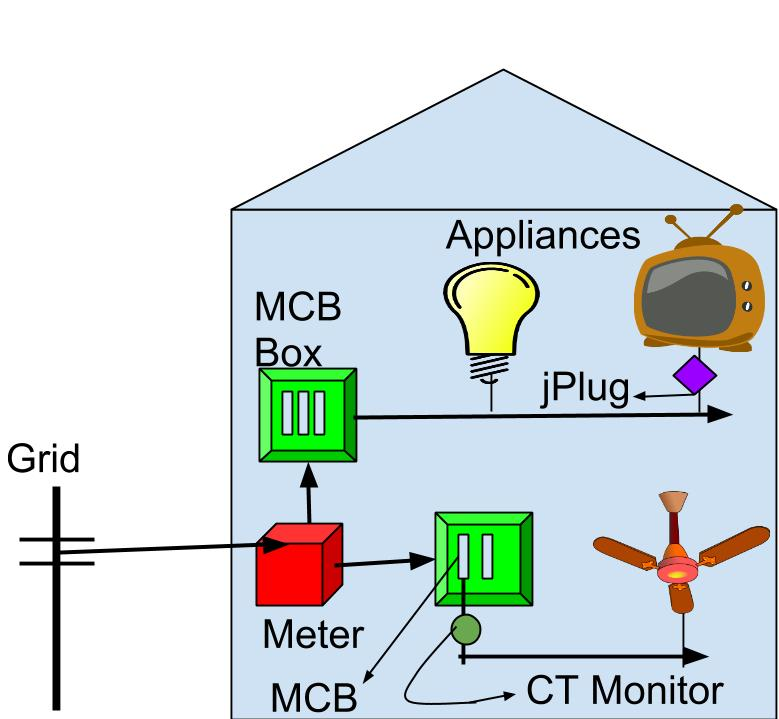
\includegraphics[scale=0.14]{./figures/electricity_distribution.jpg}}
    \hspace{1mm}
    \subfloat[\scriptsize Different granularity of measuring water consumption in home: inlet supply from utility, outlet supply from tank]{
    	 \label{fig:water_distribution}
        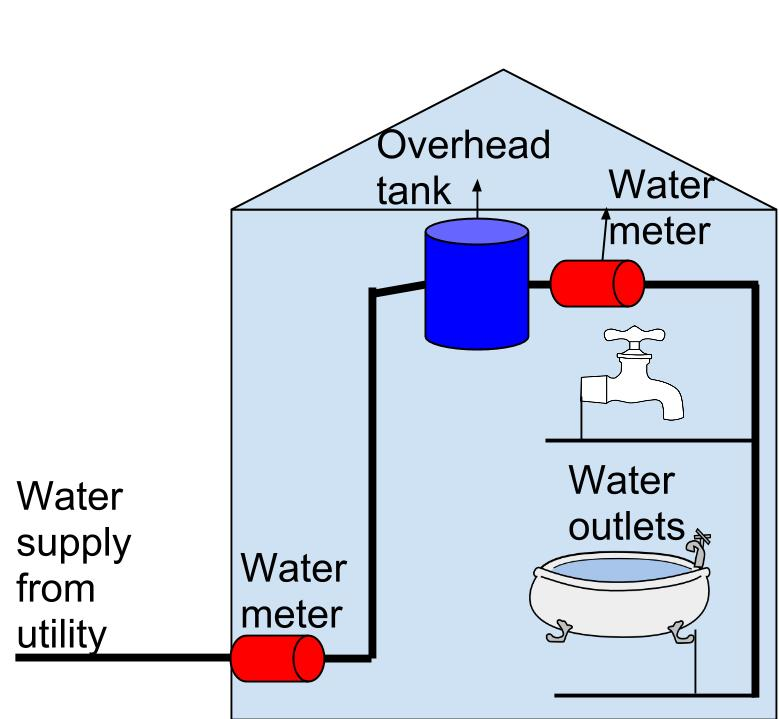
\includegraphics[scale=0.14]{./figures/water_distribution.jpg}}
        \vspace{-3mm}
   \caption{Electricity and water flow inside a home and different granularity at which these parameters can be monitored.}   
      
\end{figure}
\noindent \textbf{Water monitoring:} 
%There are a few differences in home water distribution in India when compared to developed countries. 
In India water supply is available only for a few hours a day. Thus, overhead water tanks (typically 1000 liters capacity) are used to store water, when available, and supply it for home activities throughout the day. Due to low water pressure, electric motors are used to pump the water for storage for the times when the supply is available. %Thus, the flow of water in a home can be summarized as follows: 1) Water from utility comes to the home; 2) Electric motor is used to aid in pumping the water up to the tank; 3) Water flows downward from the tank whenever water is consumed. 
\figref{fig:water_distribution} illustrates the water flow distribution, together with the placement of water meters. One water meter is placed at the inlet (coming from the utility) and another one at the outlet from the water tank (flowing downwards). %to capture the incoming (from utility) and outgoing (from tank) water consumption. 

Due to prohibitive cost and procurement difficulty for digital water meters in India, we chose to use Zenner Aquameter's multijet\footnote{\url{www.aquametwatermeters.com/multijet.html}}. The multijet uses pulse output generated through a 4-20 mA current loop. 
%Pulse output is commonly used for analog signaling in industrial process control instruments. 
For the water meter connected to the utility, over a 0.5 inch diameter pipe, a pulse is generated for every 1 liter of water consumption. Water meter connected to the outlet of storage tank, with 1.25 inch diameter, generates a pulse every 10 liters of water consumption. %generating a pulse every few liters. The precision is based on the quality of the sensor and the diameter of the water pipe. The water meter we used for overhead tank gives a pulse every 10 liters, whereas the one used for inlet supply from utility gives a pulse every 1 liter. These pulses can be measured using the circuit diagram for 4 ma loop shown in ... 
\figref{fig:water_meter} shows the water meter deployed inline at the overhead tank.

\noindent \textbf{Ambient monitoring:} We used ZWave based Express Controls HSM100\footnote{\url{http://goo.gl/Bszg0u}} multisensors for monitoring motion, light and temperature across 5 rooms in the home. Till date, to the best of our knowledge, no commercial ZWave based sensor is available working on Indian frequency (865.2 MHz). We correspondingly imported EU frequency (868.4 MHz) devices and used it for ambient monitoring. For these HSM100, motion is reported in an event-driven manner (i.e. whenever there is change in motion status, a reading is reported) and temperature and light are polled at 1 Hz. We also placed 1 Android phone at a fixed location in each room and ran FunF journal application\footnote{\url{http://www.funf.org/journal.html}} to log ambient parameters such as light and sound level every 30 seconds for 5 seconds.

\noindent \textbf{Miscellaneous:} Android phones, in addition to measuring ambient conditions, were also used to scan and log Bluetooth, WiFi and GSM networks. All home occupants were requested to keep the Bluetooth, for their personal phone, on during the duration of the experiment. The network scanning was done every 1 minute and is stored locally on the SD card. External weather conditions, such as temperature, humidity and wind speed, were also logged every 10 minutes using publicly available APIs from weather monitoring stations\footnote{Forecast, World Weather, Open Weather Map}.
%\footnote{Forecast: \url{www.forecast.io}, World Weather: \url{www.worldweatheronline.com}, Open Weather Map: \url{www.openweathermap.org}}
%Additionally, network traffic was sensed to monitor connectivity and signal strength.

%Such miscellaneous data collection, together with detailed electrical consumption, water consumption and ambient information, can be used for multiple applications including energy-apportionment (i.e. assigning energy usage to different occupants within the home), localization and correlating energy usage with outside temperature.

Complete sensing infrastructure, used in our deployment, is summarized in \tabref{tab:sensing}.


\subsection{Communication and Computation}
Our sensing infrastructure, described in \secref{sec:sensing}, involves multitude of communication channels. Different computing platforms - microcontrollers, single board computers (SBCs) (e.g. Raspberry Pi\footnote{\url{www.raspberrypi.org}} (RPi) and Ionics Stratus\footnote{\url{www.ionics-ems.com/plugtop/stratus.html}}) and desktops are used for data collection.  
%In our experience we found that using a desktop computer for collecting data from individual sensors would be an overkill in terms of cost, processing power and physical space used. Although microcontrollers are cheap and occupy little space, they do not expose enough abstractions for high level programming, are often difficult to debug and are inherently hard to multi task. We thus decided to use Single Board Computers (SBC's) for sensor data collection. We used Raspberry Pi\footnote{\url{www.raspberrypi.org}} (RPi) and Ionics Stratus\footnote{\url{www.ionics-ems.com/plugtop/stratus.html}} based SBC's. 
SBCs served as a good low cost alternative (25 \$) constituting 700 MHz ARM processors, support for Linux based distributions and allow for coding in higher level languages such as Python. %These SBC's run from SD cards whose size can be chosen as per requirement. 
We used 5 RPi and 1 Ionics Stratus plug computer as SBCs and a 2 GHz Desktop PC running Linux, as the main local server.
% where all the data was stored. %The software stack running on the SBC's and how they interacted with the main server and collected data from different sensors is described below:

\looseness -1 One RPi was connected to EM6400 using RS485-USB converter. We developed a custom program based on pyModbus\footnote{\url{www.github.com/bashwork/pymodbus}} to collect the desired parameters. %library which would serially read 80 registers, using Modbus protocol, to compute 40 electrical parameters as described in \tabref{tab:sensing}. 
All the collected parameters, together with the UTC timestamp is %stored in a local CSV file. A new CSV was created every 15 minutes. A background program would periodically try to upload CSV files older than 15 minutes, to the main server, where the data is pushed in MySQL database. This architecture for data collection - creating a new CSV periodically, uploading older CSV periodically to main server where the data is then pushed into MySQL, is used for all of our sensors connected to SBCs. We call this model 
collected using \emph{\paradigms} (\selstup) model, described in detail in section \secref{sec:architecture}. On similar lines, USB output (XML formatted) from Current Cost is received on another RPi and is communicated to the desktop server. %goes through the \paradigms architecture for data collection. %A custom Python script will store data in CSV files every 15 minutes which is then uploaded by a separate background script. 
%Although Current Cost has its own cloud based APIs, we chose to collect data from it locally, in order to avoid data losses occurring due to network failures. 

%\noindent \textbf{Current Cost data collection:} Although Current Cost has its own cloud based API's, we chose to collect data from it locally, in order to avoid data losses occurring due to network failures. Current Cost provides power data in xml format over the serial interface. We thus connected the USB cable-out from the Current Cost receiver to RPi and wrote a simple Python script to read data serially using pySerial\footnote{\url{www.pyserial.sourceforge.net}} and store it in a CSV file along with UTC timestamp. CSV creation and uploading to central server was done in a similar fashion as was done for EM6400.

Two RPi were used to connect to the microcontroller based circuit monitor to read the data over the serial port and process it further using \selstup.
% One of the RPi connected to the meter was also used for circuit monitoring using the CTs in the same panel. 
GPIO headers on two more RPis were used to interface with each water meter respectively for collecting pulse output over the 4-20 mA current loop interface. We initially wrote an interrupt driven program in Python to detect 10 liter and 1 liter events for the tank and supply water meters respectively. We observed that noise introduced in the circuit due to long cable lengths led to a lot of false events. Correspondingly, we modified our program and polled at a frequency of 5 Hz to obtain GPIO status. The RPi collecting CC data was also used to collect data from the water meter attached to the supply.% and further processed this data using \paradigm.	 
%\noindent \textbf{MCB data collection:} Our custom built CT based monitor for collecting current data from different MCB's exposes data serially which is read using pySerial on a RPi and processed further using \paradigm.

A web daemon, running on the server, listened to the HTTP post request from jPlugs and dumped the data in MySQL. Ionics Plug Computer was used to collect data from all the ZWave based sensors. We wrote custom wrappers around OpenZWave\footnote{\url{www.code.google.com/p/open-zwave}} to collect temperature and light information on per second basis, and motion information based on events. While the plug computer had an internal ZWave (the reason for which it was selected), its range was limited and did not cover all the ZWave sensors. Correspondingly, a ZWave controller was connected over USB with Ionics that provided reachability to all the ZWave devices. %and the data was processed further using \paradigm. 
\figref{fig:plug} shows the plug computer collecting ambient sensor data from ZWave controller. A manual dump of collected data on each Android phone was performed every 15 days.
% We also collected weather data from 3 different weather stations.
%Electricity failure and unreliable internet are well known problems in India and are highlighted in \secref{sec:learning}. Owing to these problems, we chose to collect weather data from 3 different weather stations, in one of the servers hosted by our collaborators in the USA. 


%\noindent \textbf{jPlug appliance data collection:} jPlug makes a HTTP post every second with upto 10 electrical parameters. We saved this data directly on the server machine where a web daemon listened to requests from jPlug and dumped them in MySQL.

%\noindent \textbf{Water data collection:} Based on circuitry explained in \secref{sec:sensing}, we used GPIO header on RPi and wrote an interrupt driven program in Python to detect 10 liter and 1 liter events for the tank and supply water meters respectively. We found that noise introduced in the circuit due to long cable lengths led to a lot of false events. Thus, we modified our program and polled at a frequency of 5 Hz to obtain GPIO status and further processed this data using \paradigm.	

%\noindent \textbf{Homeseer HSM100 data collection:} We wrote custom wrappers around OpenZWave\footnote{\url{www.code.google.com/p/open-zwave}} program to collect temperature and light information on a per second basis, and motion information based on events. ZWave controller which controls all the ZWave based sensors was connected to the plug computer over USB. Data was processed further using \paradigm. \figref{fig:plug} shows plug computer collecting ambient sensor data from ZWave controller.

%\noindent \textbf{Android data collection:} We used FunF journal which would store data inside phone's SD card. We would take a dump once every 15 days and empty the SD card for further data collection.


A lot of issues, pertaining to SBCs, were observed in our deployment. As an example, the OpenZWave program that we used created log files for its own diagnostics, that eventually consumed the 512 MB flash drive space on the plug computer. This was fixed eventually by deleting older logs. Such problems encouraged us to develop soft-sensor~\cite{softgreen} streams, whereby we collected hard disk space, ping success, CPU utilization, remaining RAM space and temperature of the processor, for all the computing devices including the server at regular intervals. These soft-sensor streams can be used for offline analysis as well as for real time alerting and fault diagnosis. Similar soft-sensor streams have also been used in the previous work~\cite{hitchhiker_residential} for raising alerts.

Similar to prior research, reporting WiFi discontinuity in homes in the USA~~\cite{hitchhiker_residential}, we also observed that one WiFi router did not provide complete coverage for our 3 storey home. We thus used 3 Netgear JNR1010\footnote{\url{www.support.netgear.com/product/JNR1010}} routers, where the router on the first floor acted as the host and the routers on the ground and the second floor were bridged to it. %More details regarding the need of multiple routers and network availability in homes is described in \secref{sec:learning} and \secref{sec:common}.

\vspace{-1mm}
\section{System Architecture}	
\label{sec:architecture}
Middleware systems such as sMAP~\cite{smap}, BuildingDepot~\cite{buildingdepot} and SensorAct~\cite{Arjunan12} have been proposed in the past for sensor data collection. However, we found that they do not sufficiently address the requirements of our deployment context e.g. faulty internet and repeated power failures. Motivated by our experience as well as previous work from other researchers~\cite{hitchhiker_residential}, where importance of simplifying the architecture are proposed, we propose \paradigms (\selstup) model. \selstups involves two main ideas- local storage (on SBCs) and periodic data upload (from SBC to server, and from server to cloud). Data collected from the sensors was \textbf{locally stored} in the form of comma separated value files (CSV), in SBCs and \textbf{periodically uploaded} to the main desktop server. In case the upload failed, it was retried after a fixed time duration. Each SBC was provisioned with sufficient flash based local storage to accommodate sensor data for a few days, to account for persistent upload failure.
\begin{figure*}[t!] 
    \vspace{-11mm}
    \hspace{-2mm}
    \subfloat[\scriptsize Power outage vs Time]{
    \label{fig:failure_time}
    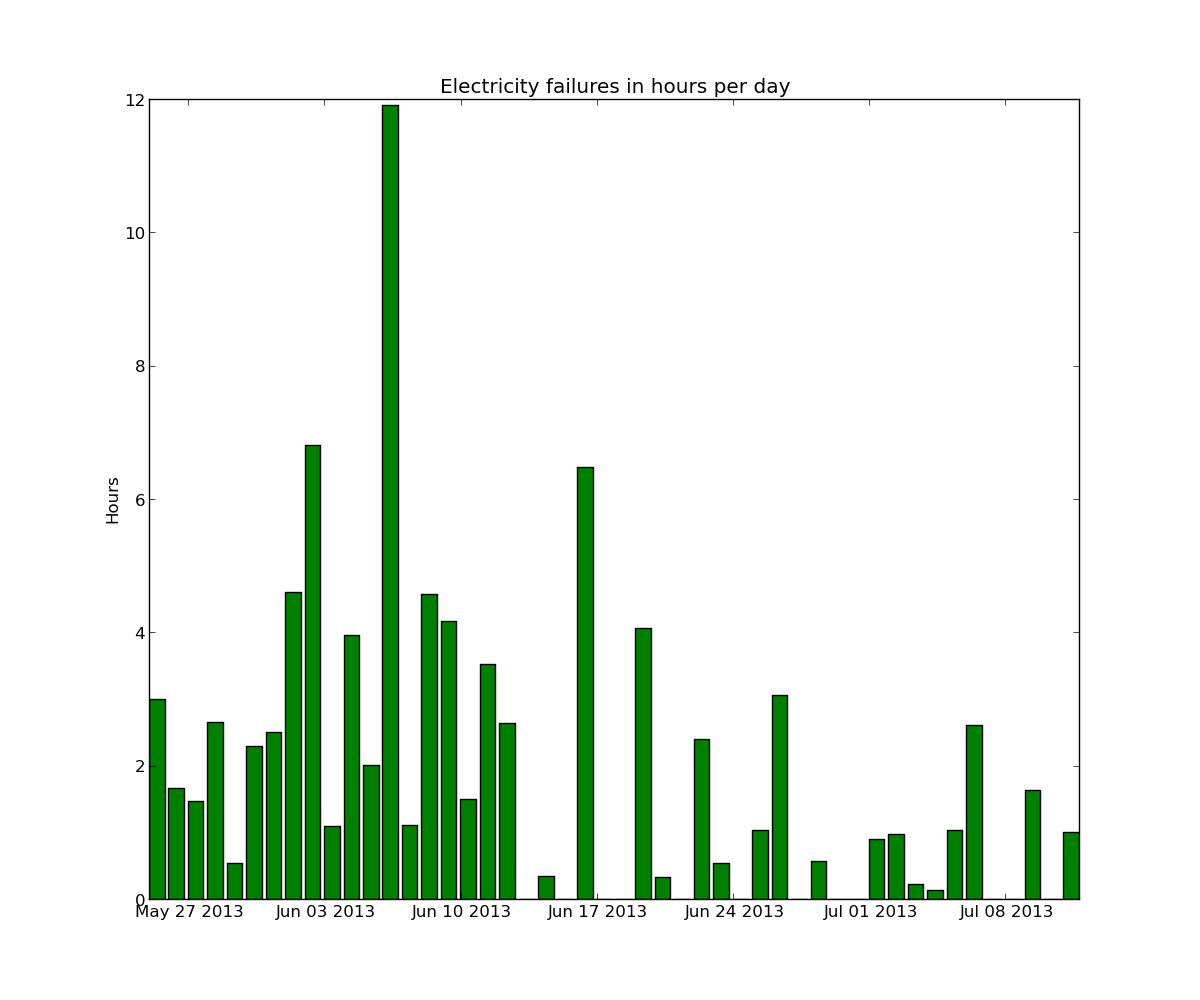
\includegraphics[scale=0.12]{./figures/electricity.png}}
    \hspace{-1mm}
     \subfloat[\scriptsize Power outage duration ]{
        \label{fig:failure_duration}
        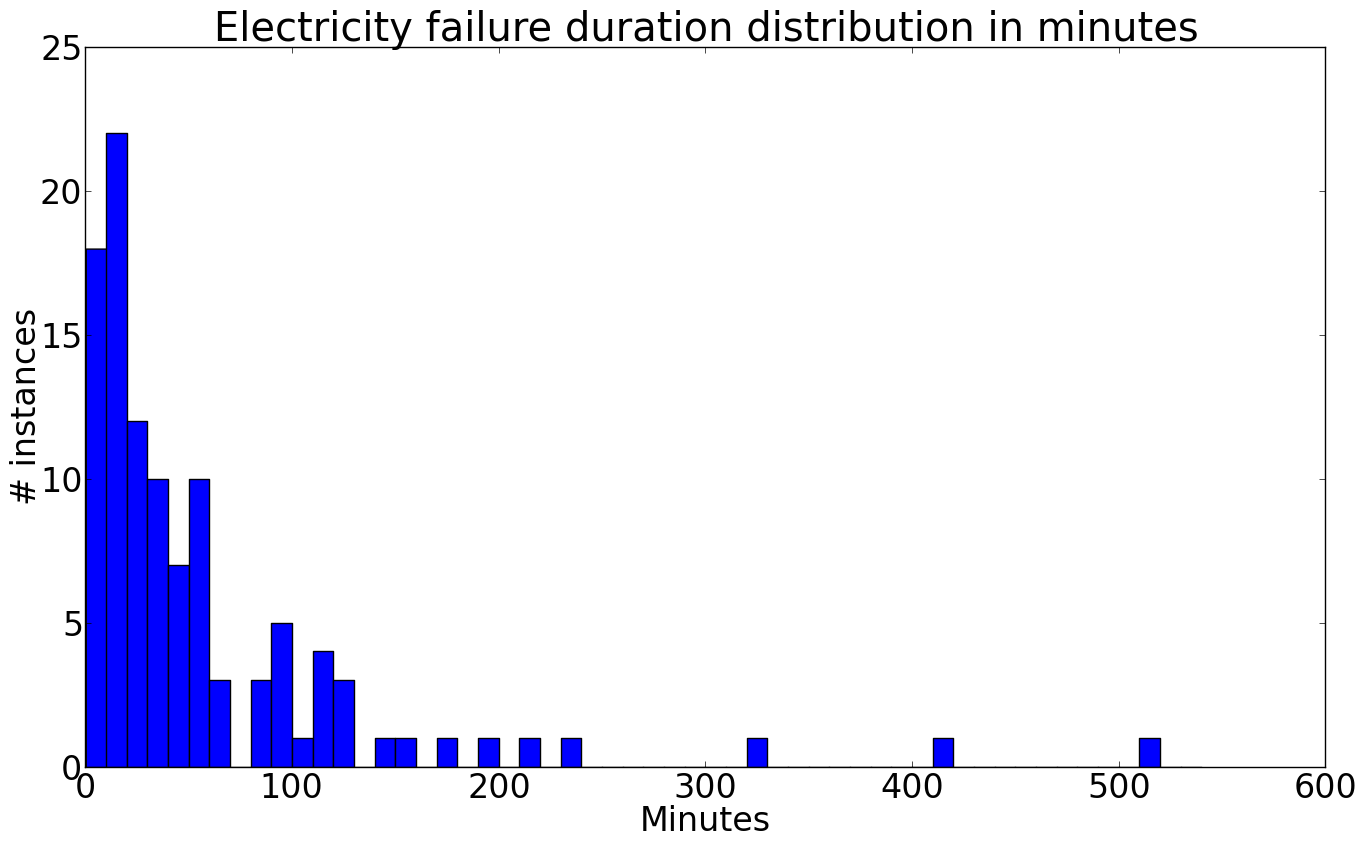
\includegraphics[scale=0.12]{./figures/failure_durations.png}}
       \hspace{-1mm}
     \subfloat[\scriptsize Power outage by hour of day]{
             \label{fig:failure_hour}
             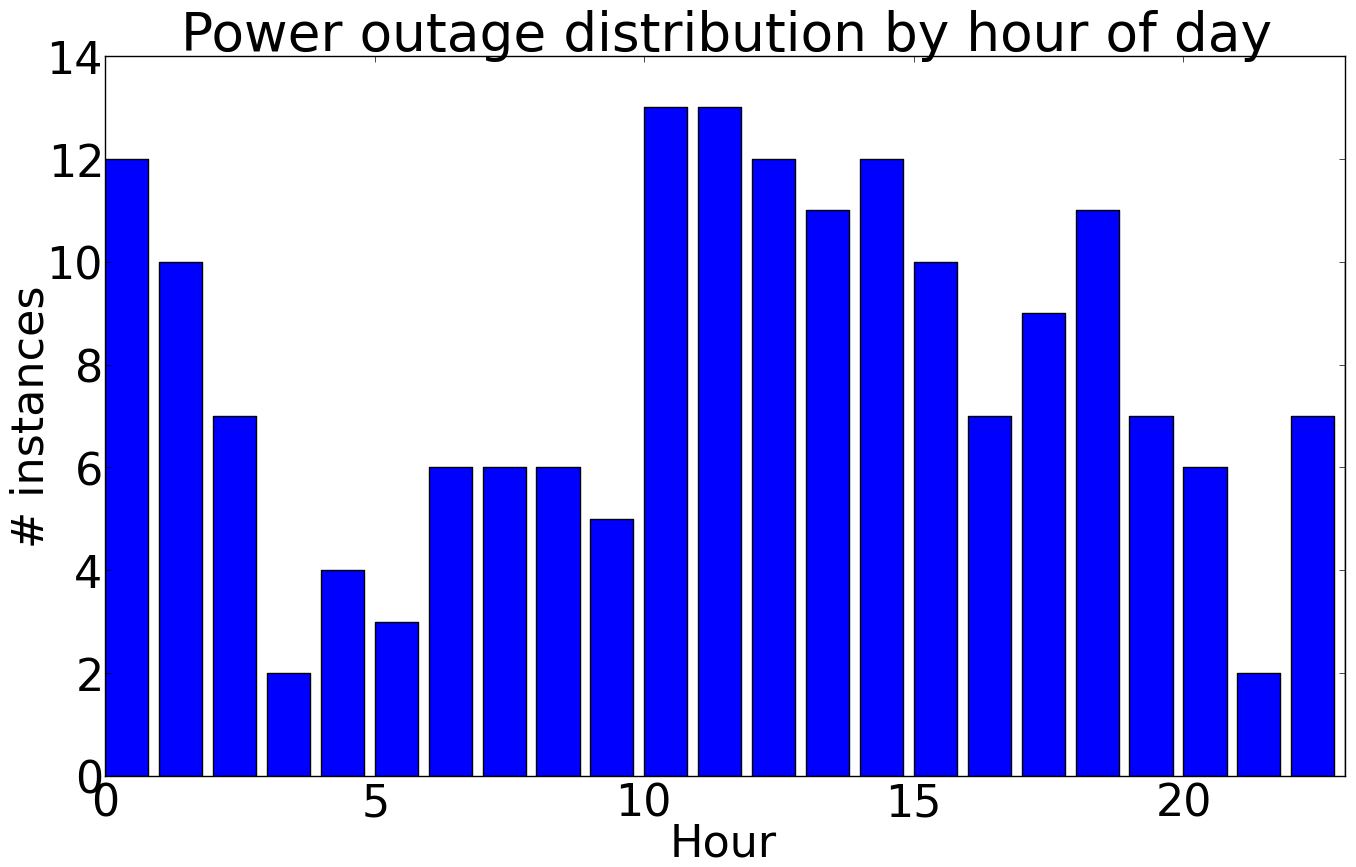
\includegraphics[scale=0.12]{./figures/outage_by_hour.png}}
%             \hspace{-1mm}
       \subfloat[\scriptsize Voltage fluctuations in a week in our deployment]{
                                             \label{fig:voltage_box}
                                             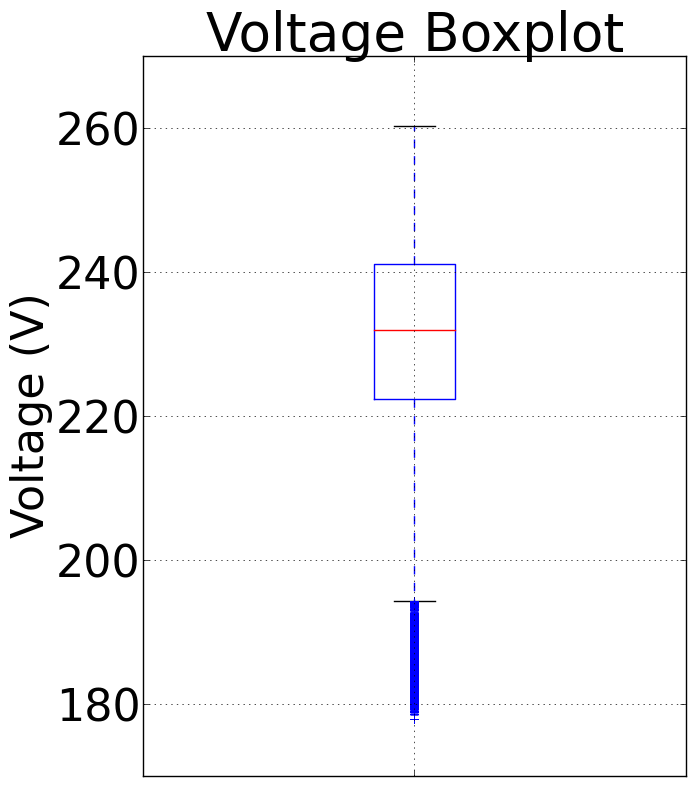
\includegraphics[scale=0.135]{./figures/voltage_box.png}}
         \hspace{1mm}
               \subfloat[\scriptsize Voltage fluctuations in a week in SMART* dataset]{
                                                     \label{fig:voltage_box_us}
                                                     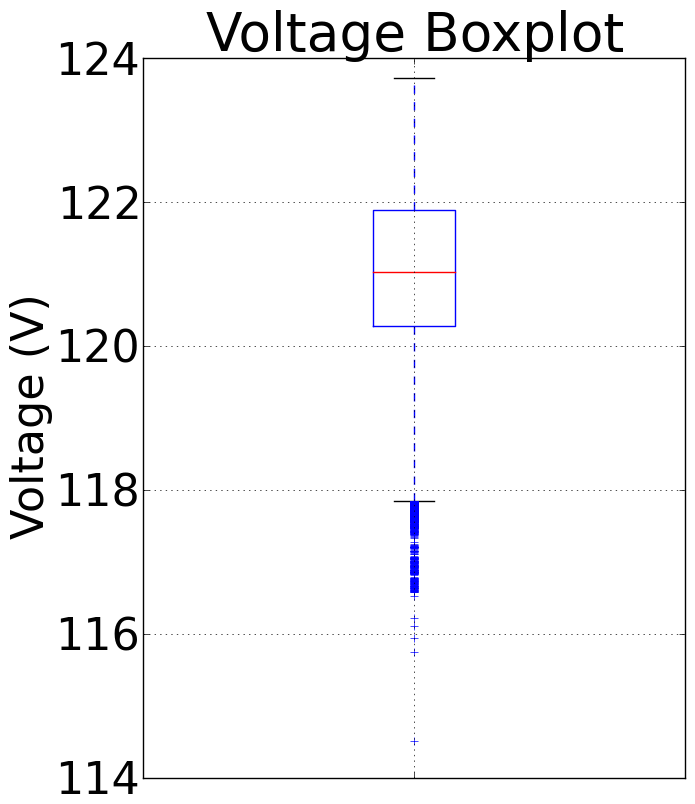
\includegraphics[scale=0.135]{./figures/us_voltage_box.png}}
              \vspace{-4mm}
               \hspace{-2mm}
             \newline      
                  
          \subfloat[\scriptsize Voltage fluctuations on one of the days in our deployment]{
                  \label{fig:voltage}
                  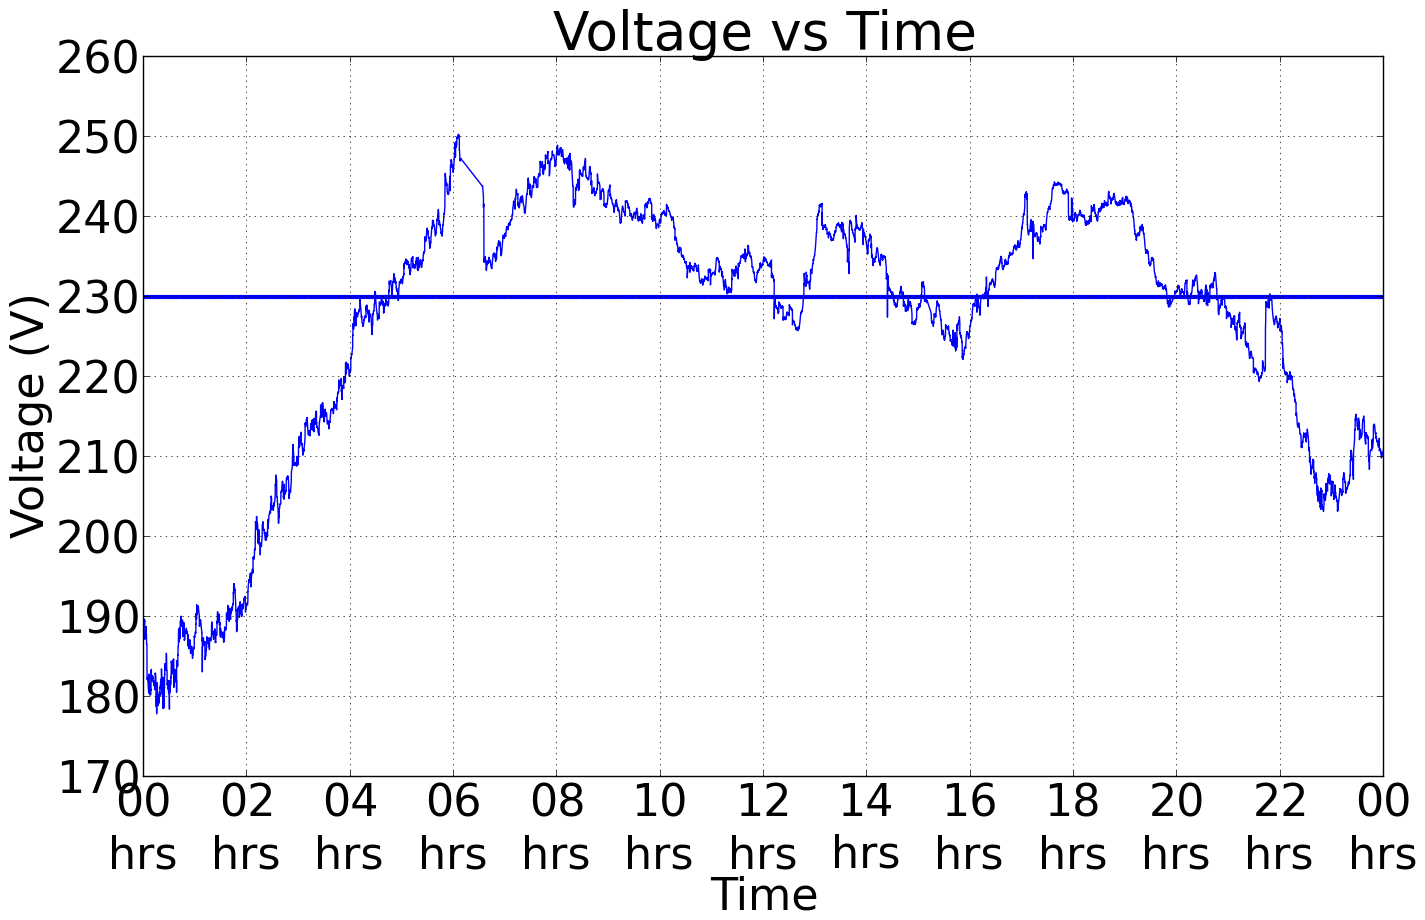
\includegraphics[scale=0.12]{./figures/voltage.png}}
                  \hspace{-1mm} 
            \subfloat[\scriptsize Voltage fluctuations on one of the days in SMART* dataset]{
                              \label{fig:voltage_us}
                              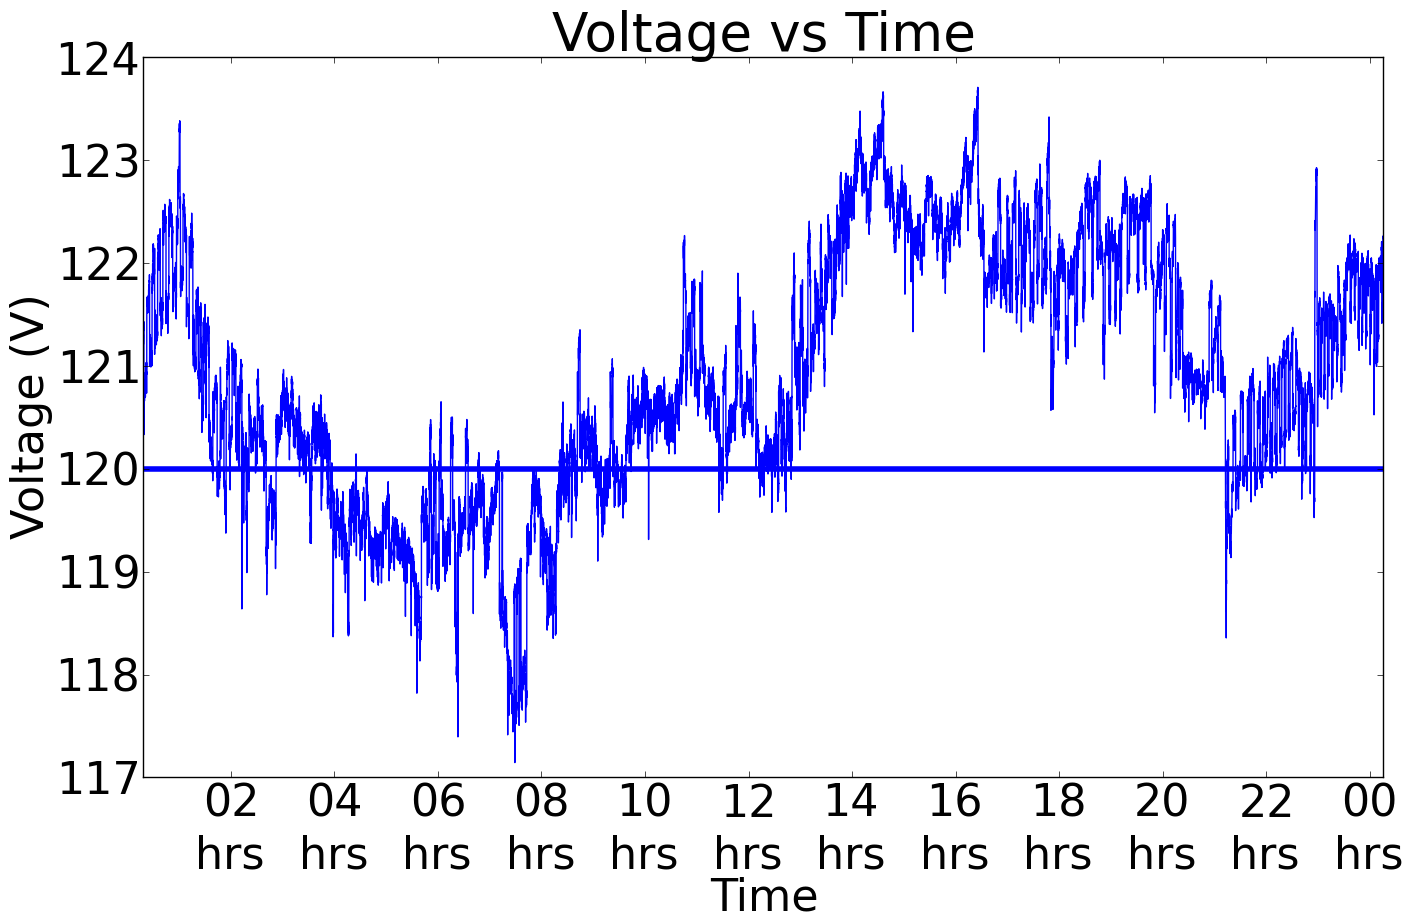
\includegraphics[scale=0.12]{./figures/us_voltage.png}}
                  \hspace{1mm}
          \subfloat[\scriptsize Observed voltage just before power outage during night hours (10 PM to 1 AM)]{
                                      \label{fig:voltage_before_outage}
                                      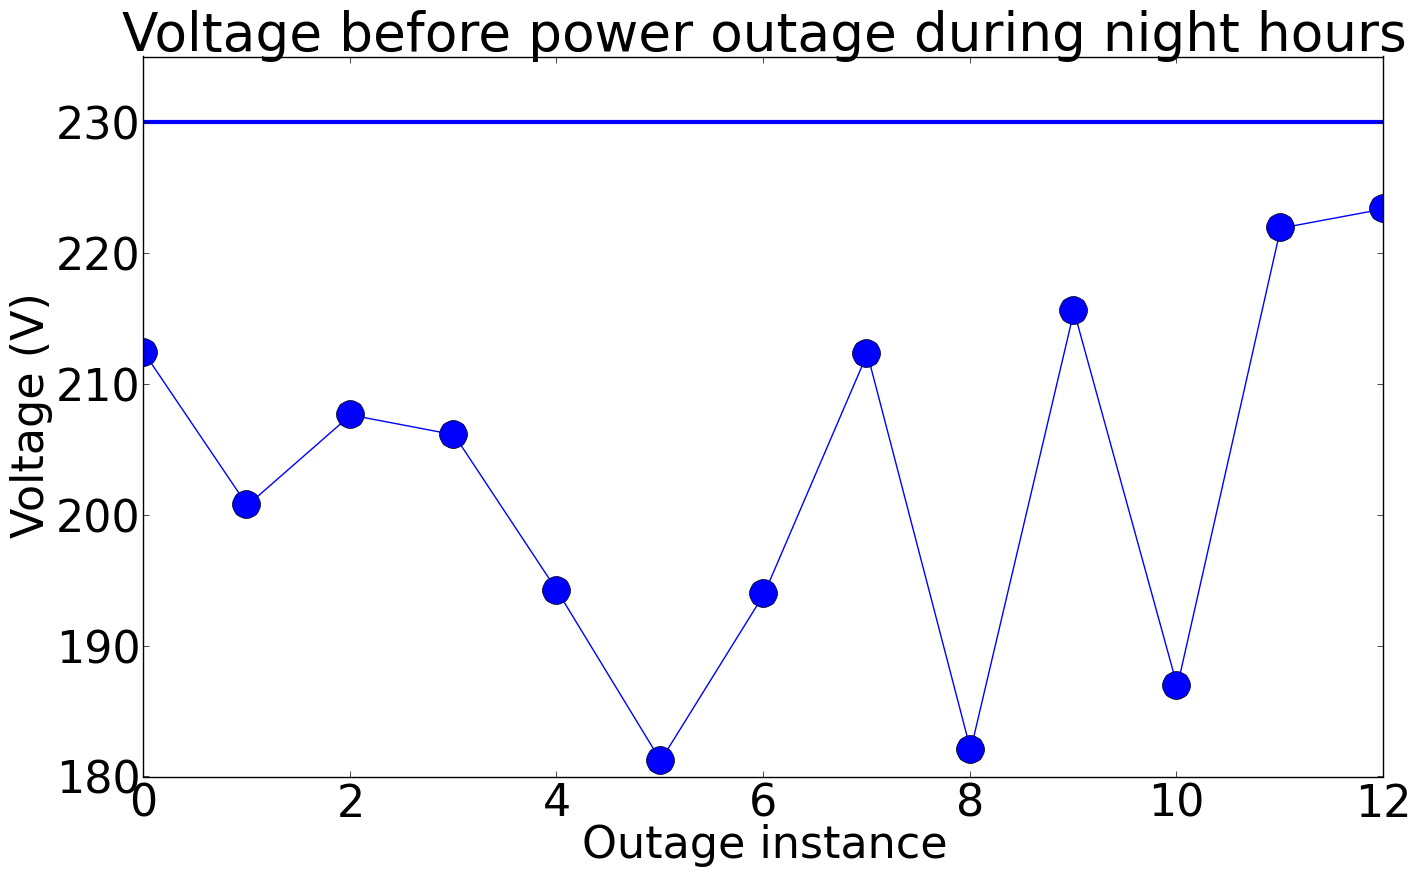
\includegraphics[scale=0.12]{./figures/voltage_before_outage.png}}
          \subfloat[\scriptsize Frequency fluctuations in a week in our deployment]{
                            \label{fig:frequency_box}
                            \hspace{2mm}
                            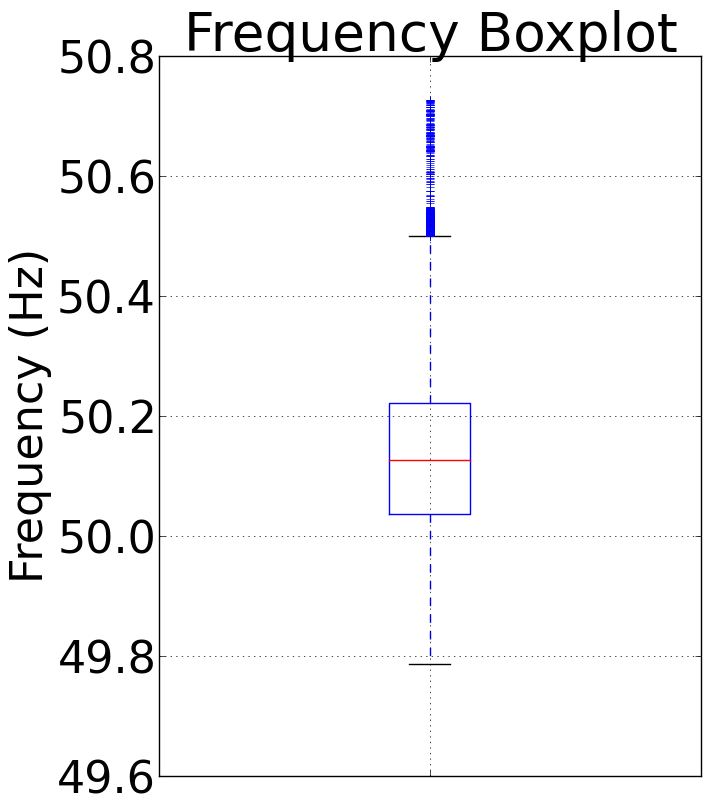
\includegraphics[scale=0.135]{./figures/frequency_box.png}}
		\subfloat[\scriptsize Frequency fluctuations in a week in SMART* dataset]{
		                            \label{fig:frequency_box_us}
		                            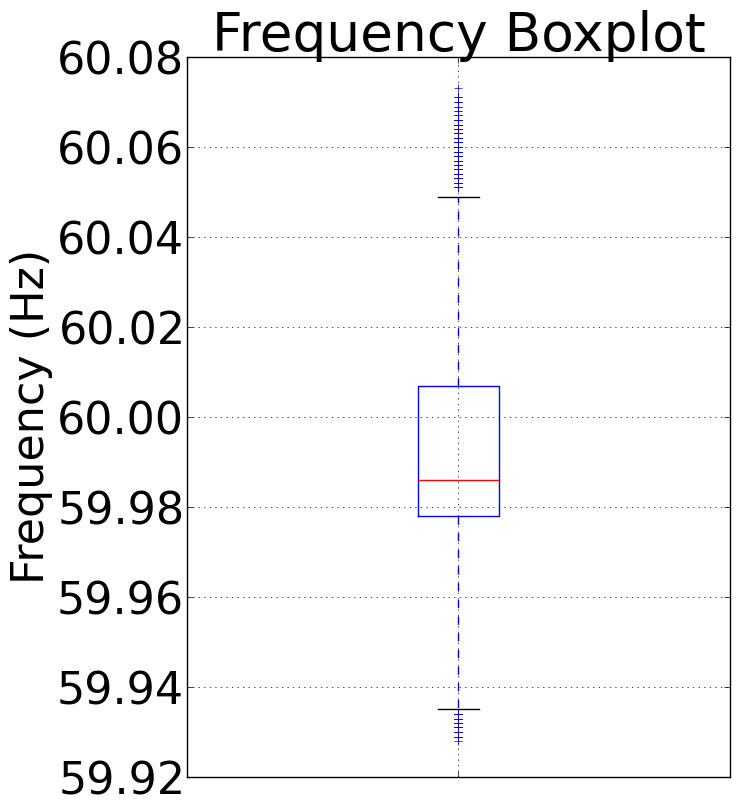
\includegraphics[scale=0.135]{./figures/us_frequency_box.png}}                           
          
                            
     \vspace{-3mm}
   
    \caption{Unreliable grid. Rated voltage in India and US are 230V and 120V respectively. Rated frequency in India and US are 50Hz and 60Hz respectively}

    \label{fig:unreliable}

\end{figure*}

% % % % % % % % % % % % % % % FIGURE CONTAINING ARCHITECTURE + # Data packets % % % % % % % % % % % % % % % % % % % % % % % % % % % % %
%\begin{figure}
%\vspace{-8mm}
%\subfloat[\scriptsize \paradigm]{
%    \label{fig:architecture}
%    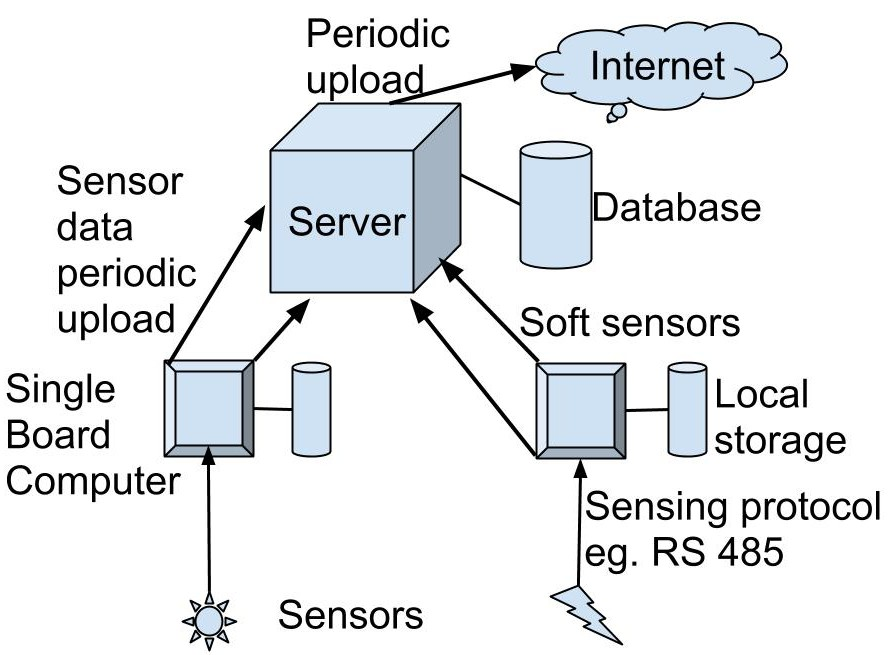
\includegraphics[scale=0.13]{./figures/architecture.jpg}}
%        \subfloat[\scriptsize Amount of data (worth seconds) collected per day from water meter. Data worth 86400 seconds is expected per day. Note that limits on yaxis are raised to ensure that power outage and software losses are visible]{
%        \label{fig:architecture_efficacy}
%        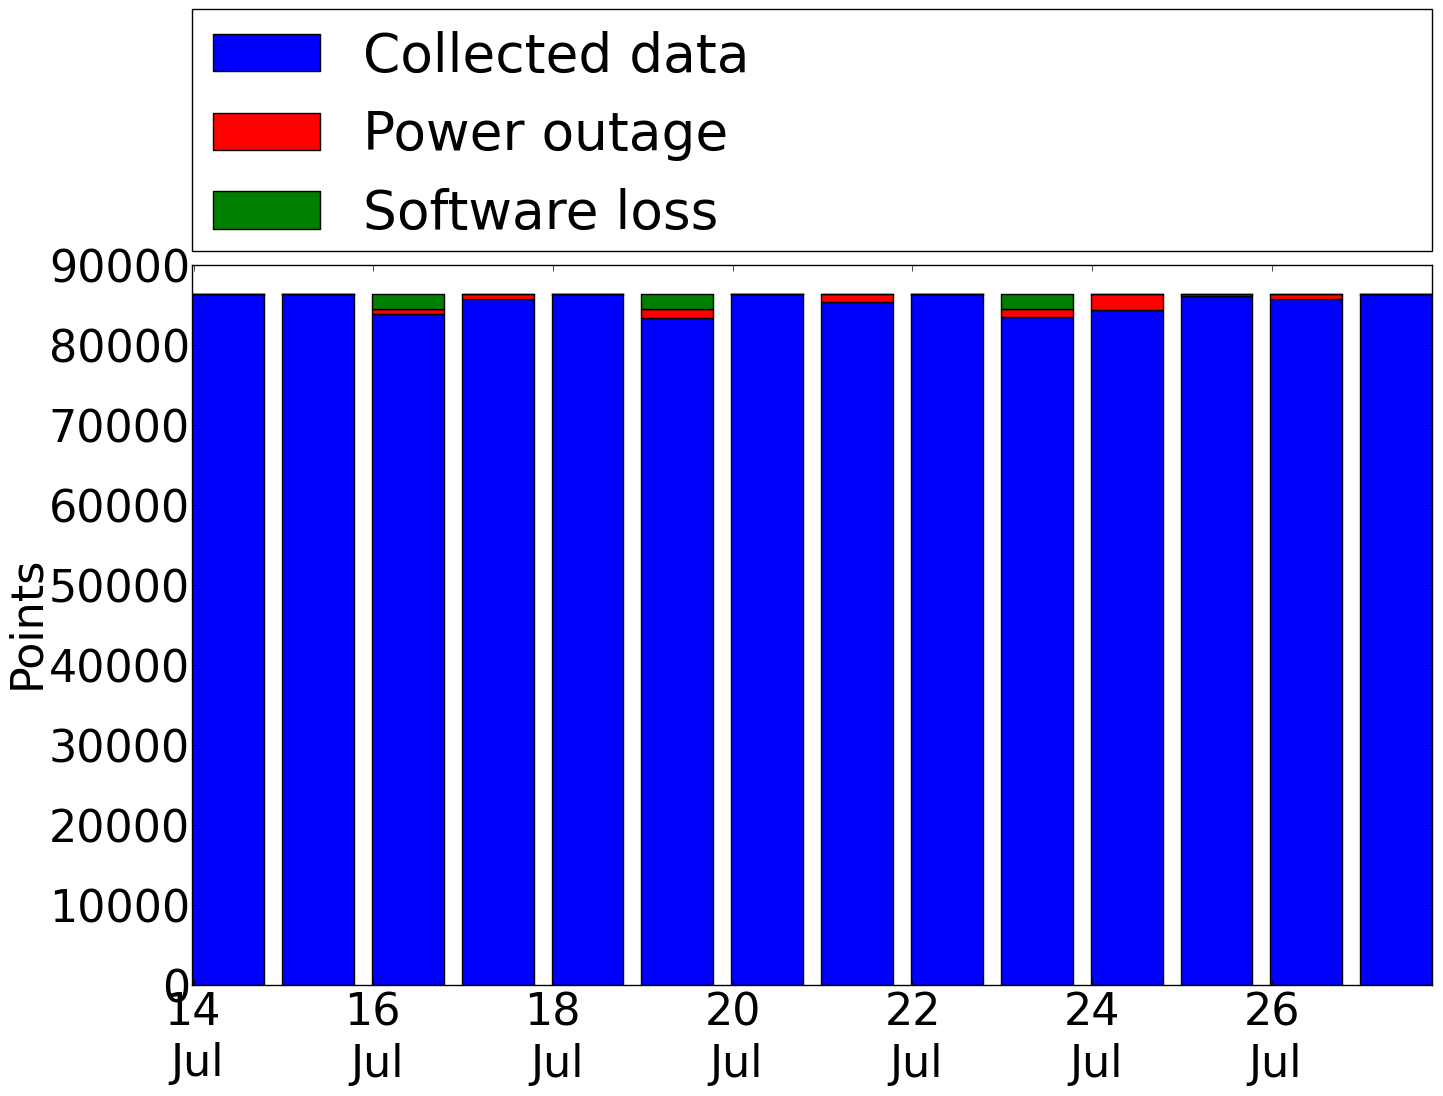
\includegraphics[scale=0.125]{./figures/data_loss.png}}
%        \vspace{-3mm}
%  \caption{\paradigms architecture and its impact on ensuring no data loss}
%  \vspace{-2mm}
%   
%\end{figure}
% % % % % % % % % % % % % % % % % % % % % % % % % % % % % % % % % % % % % % % % % % % % % % % % % % % % % % % % % % % % % % % % % % % %

\begin{figure}

\centering 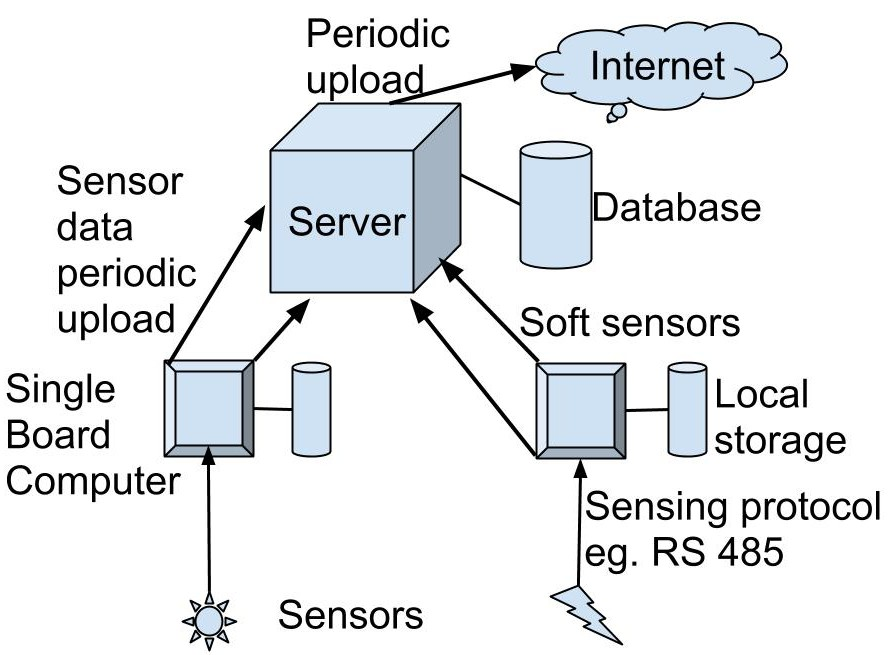
\includegraphics[scale=0.13]{./figures/architecture.jpg}
\vspace{-2mm}
\caption{\paradigms architecture}
\vspace{-2mm}
\label{fig:architecture}
\end{figure}



Web applications running on the server allowed residents to locally visualize their data from multiple sensing streams. Data from the server was periodically replicated to the cloud, allowing researchers to remotely visualize the data and maintain the deployment. \figref{fig:architecture} illustrates the \selstups architecture. The salient features of our architecture are:


\noindent \textbf{Decoupled sensing and data uploading:} ensuring that an error in data uploading does not impact the sensing and vice versa, avoiding data loss due to network (even local in-home WiFi) failure. The design choice of decoupling comes from the well established principles of software engineering.

\noindent \textbf{Minimal internet requirement:} Internet is required \textbf{only} when outside researchers wish to view data in near-realtime. Internet failure does not have any impact on robust sensor data collection. The periodic nature of our uploads ensured that data would be uploaded when internet connectivity is re-established. Local storage, on SBC, further ensures reliable data collection, even in the cases of server failure. %Further, there is no data loss even if the server goes down for some time, due to local storage.

\noindent \textbf{Reduced load on server:} Periodic upload of data (in larger volumes) results in reduced computation and bandwidth requirements for the SBCs and the server. 
%While it comes at the cost of increased storage requirements on SBCs, our analysis shows that 1 GB of local storage will suffice for most of the practical scenarios. %, we did not need to provision for more than 1 GB.

In our experience, we found that the novel features of \selstups prevented data loss due to internet, server downtime, etc. We had accidentally killed the server script for taking CSV data from RPis collecting water data. However, when we rectified that, within 1 hour all the data for previous 1 week, which had been locally stored on the RPi was eventually collected on the server. 

%\figref{fig:architecture_efficacy} shows the amount of data collected from the water meter during that week.\redcolor{possibly remove the figure, eats up space and does not add much value beyond explanation; moreover can be confusing to the reviewer sparking doubts}


\vspace{-1mm}
\section{How is this deployment different?}
\label{sec:learning}
We now discuss some of the key unique aspects brought forward from our deployment. 



\noindent \textbf{Unreliable electrical grid:} Load shedding or rolling blackout is commonplace in the developing countries. %owing to several reasons such as improper infrastructure management, high demand and low electricity production. 
Specifically in India, power outages are common in summers when the load is high due to excessive usage of air conditioners. Excessive load and poor infrastructure also leads to significant fluctuations in the supply voltage. %As a result, voltage fluctuations or brownouts are also common.

Various statistics, collected from our deployment, further establish these aspects. We used multiple sources, such as, Unix \emph{last} command (which provides a history of boot times) on the desktop server, common missing data duration from multiple sensors, to find power outages reliably. \figref{fig:failure_time} shows power outages in number of hours per day during June-July 2013. One of the days experienced power outage for up to 12 hours (the situation is worse outside of the major cities in India, with electricity coming only for a few hours every day). \figref{fig:failure_duration} shows the distribution of power outages duration. A total of 107 power outages were reported in the 61 day period. While the average power outage lasted about 1 hour, there were outages lasting upto 9 hours. \figref{fig:failure_hour} shows the power outage distribution by hour of the day, showing maximum outages around 10 AM in the morning and around midnight. These times correspond to office time and night time when air conditioners in offices or homes are turned on leading to excessive demand on the grid. \figref{fig:frequency_box} and \figref{fig:voltage_box} show frequency and voltage fluctuations for a week in June from our deployment. We compare them with the frequency and voltage fluctuations for a week from SMART* dataset shown in \figref{fig:frequency_box_us} and \figref{fig:voltage_box_us} respectively. We can observe that there is a lot more fluctuation in both these parameters in the Indian setting. \figref{fig:voltage} and \figref{fig:voltage_us}  show voltage fluctuations on one of the days from our deployment and the SMART* dataset respectively. 

%\figref{fig:voltage} shows the voltage fluctuations, between 180 and 250 Volts, as observed on a typical day. \redcolor{Is it really a typical day? Can you do a box plot for voltage fluctuations for maybe one of the weeks - that will probably have more impact.} 
Significant amount of NILM literature uses current data
%, as measured at different granularity, 
for disaggregation. This has an inherent assumption of almost fixed voltage from the grid. \emph{Observed voltage fluctuations motivate two important aspects - 1. Load measurement devices should measure both current and voltage and not only current as is done in many of the CT based devices; and 2. When performing disaggregation, normalization to account for voltage fluctuations (as was proposed in the original NILM work~\cite{hart}) is important.}
%We observe that voltage drops during the peak load hours. 
\figref{fig:voltage_before_outage} shows that voltage just before the power outage (for a selected sample of outages occurring in the  from 10 PM to 1 AM). We observe that the voltage is well below the rated voltage of 230 V. This is in coherence with previous work~\cite{nplug}, which hypothesized that frequency and voltage measured at the home level are potential indicators of the load on the grid.

\noindent Due to unreliable nature of the grid, we wanted to ensure that all our systems were capable of automatically restarting after a power outage. Data collection and upload scripts were executed during startup. This feature further provided us with another advantage - when the system was observed to be down, we just asked the home occupant to cycle power to the system. This ensured that there was minimal data loss till the time researchers could visit the site and diagnose the fault. Appropriate logs in the scripts ensured that the fault could be diagnosed in an offline manner.  With several devices, each with its diverse sensing, computation and communication requirements, ensuring this reliability at the system level was observed to be non-trivial. Our experiences demonstrate how \emph{a robust building monitoring and control system can ensure system recovery after power failure.}

\begin{figure}
\vspace{-4mm}
\subfloat[\scriptsize \% internet packet drop vs time]{
    \label{fig:network}
    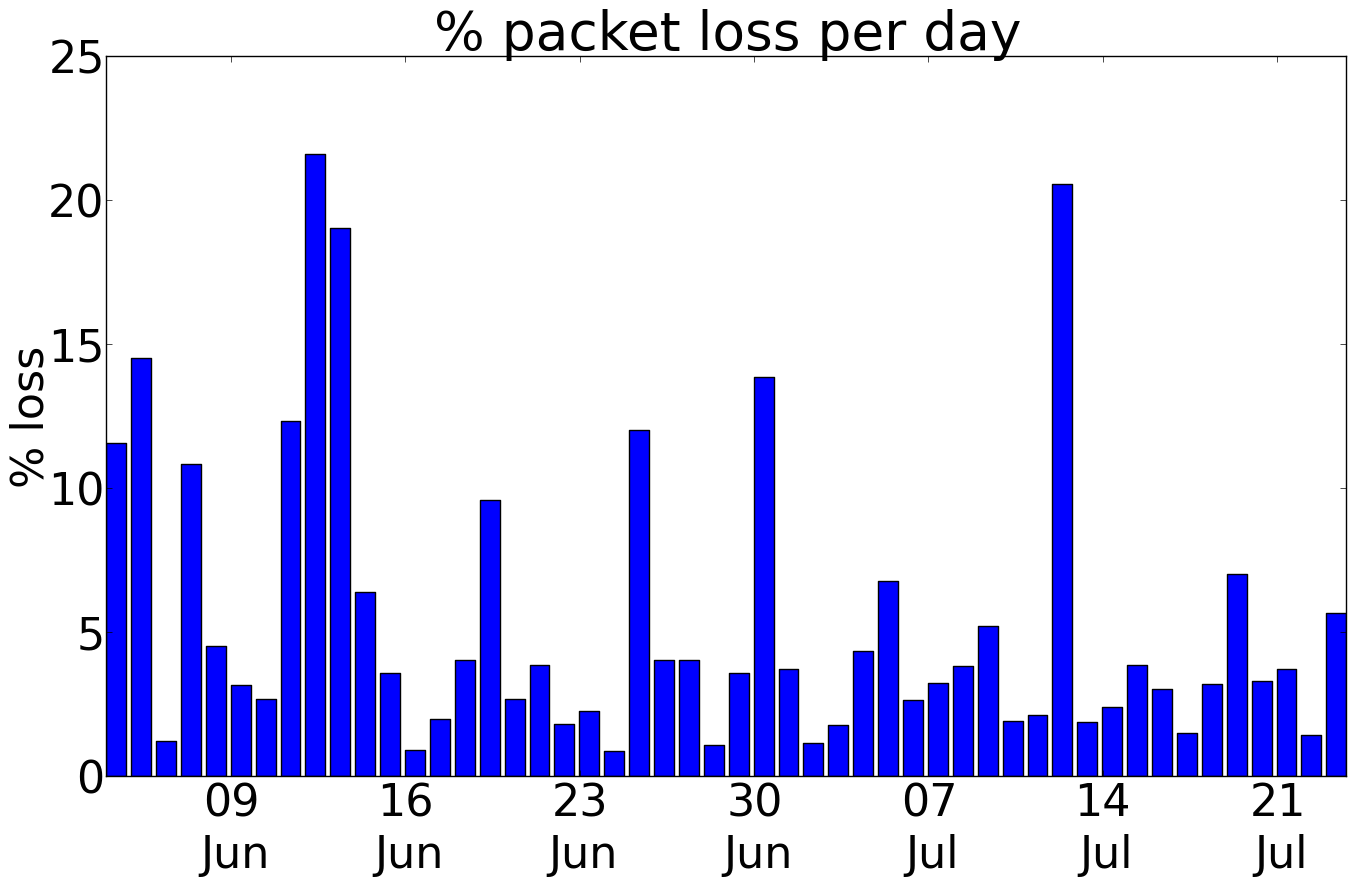
\includegraphics[scale=0.11]{./figures/network.png}}
        \subfloat[\scriptsize \% internet packet drop CDF]{
        \label{fig:network_hist}
        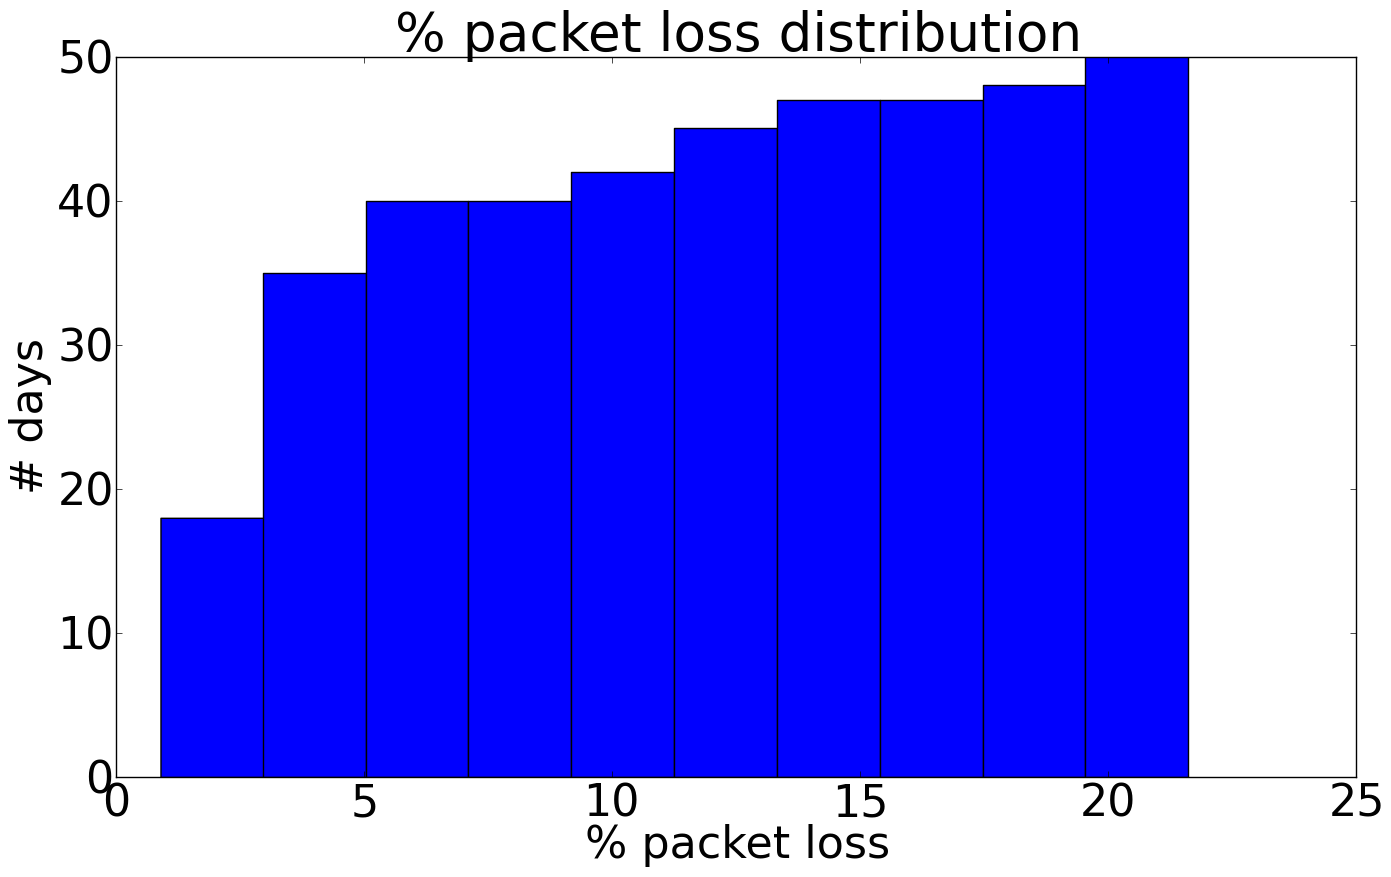
\includegraphics[scale=0.11]{./figures/network_hist.png}}
        \vspace{-3mm}
  \caption{Unreliable internet}
  \vspace{-2mm}
  
      \label{fig:unreliable_internet}
\end{figure}

\noindent \textbf{Unreliable network connectivity:} While India has one of the fastest growing internet user base, only 11\% of the total population is connected to internet (the corresponding figure in USA is 78\%)~\cite{meyer}. %Average connection speed in India is 1.3 Mbps, the corresponding numbers in developed countries are in excess of 10 Mbps~\cite{state_of_internet}. 
%Even though the condition of internet has vastly improved in the previous few years, from practical experience, we have found it to unreliable. 
We observed internet was either unavailable or had a slow intermittent connectivity periodically throughout the day. We collected network statistics by performing 15 internet ping requests every 15 seconds and computed packet drop. \figref{fig:network} shows that packet drop of up to 22\% was observed on certain days. The average packet drop per day was approx. 6\%. \figref{fig:network_hist} shows a CDF plot of \% packet drop. It can be seen that approx. one-fifths of total days reported greater than 10\% packet loss. Unreliable internet was the prime motivation behind the proposed \selstups model, discussed in \secref{sec:architecture}. Based on our experience with the proposed model, we believe that for a building monitoring and control system to scale up for the context in developing countries, \emph{the \selstups model should be adopted rather than completely relying on good internet connectivity.} %We, thus, believe that for deployments where internet is unreliable, architectures such as \paradigms should be adopted.
%
%\noindent To measure the network connectivity, we collected network statistics by performing 15 internet ping requests every 15 seconds and collected the statistics on packet drop. \figref{fig:network} shows that packet drop of up to 22\% was observed on certain days. The average packet drop per day was approx. 6\%. \figref{fig:network_hist} shows a CDF plot of \% packet drop. It can be seen that approx. one-fifths of total days reported greater than 10\% packet loss. 


\begin{figure}
\vspace{-4mm}
\subfloat[\scriptsize Before repair]{
    \label{fig:before_repair}
    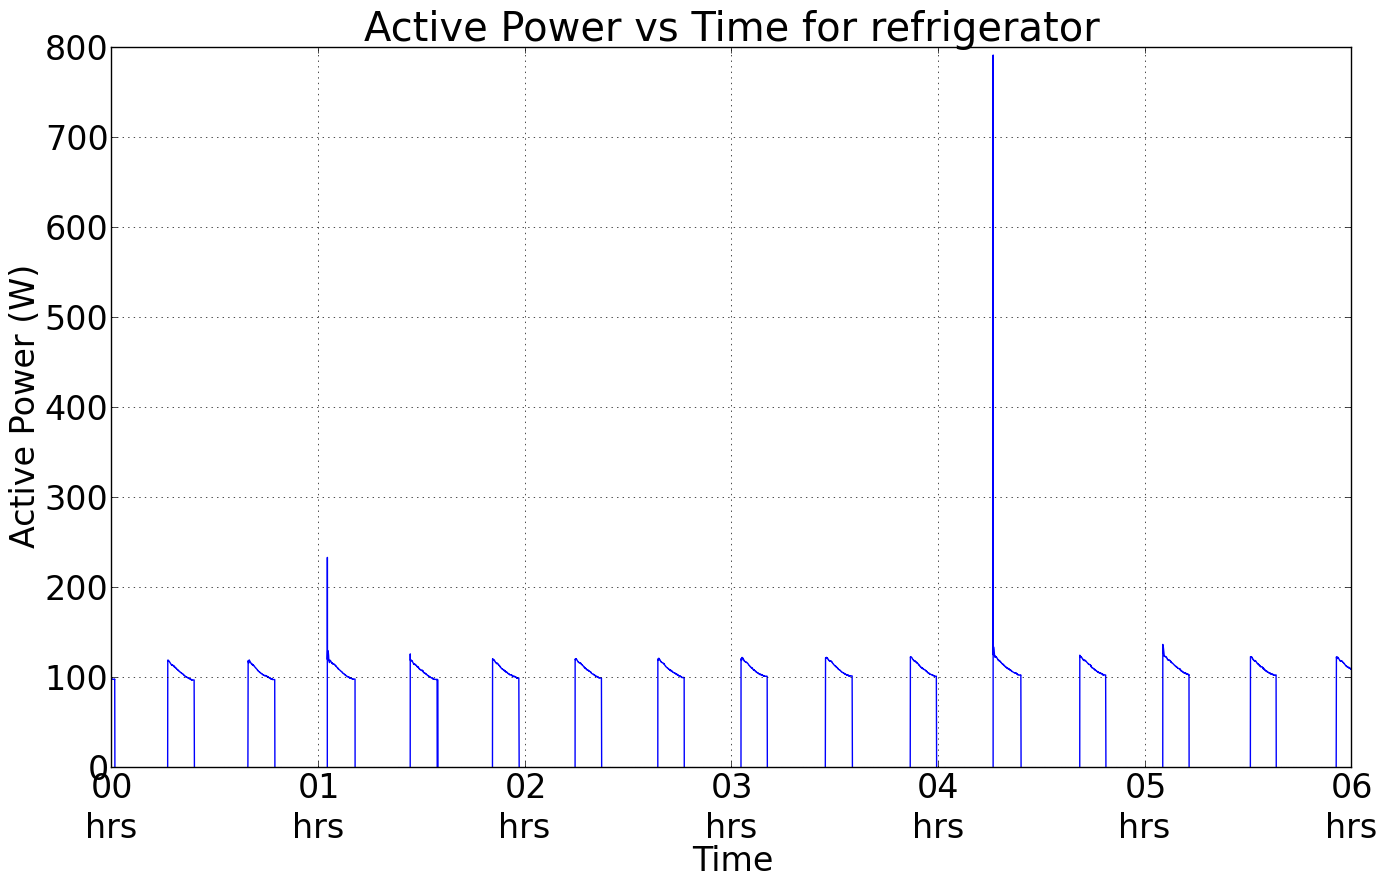
\includegraphics[scale=0.1]{./figures/before_repair.png}}
     \subfloat[\scriptsize After repair ]{
        \label{fig:after_repair}
        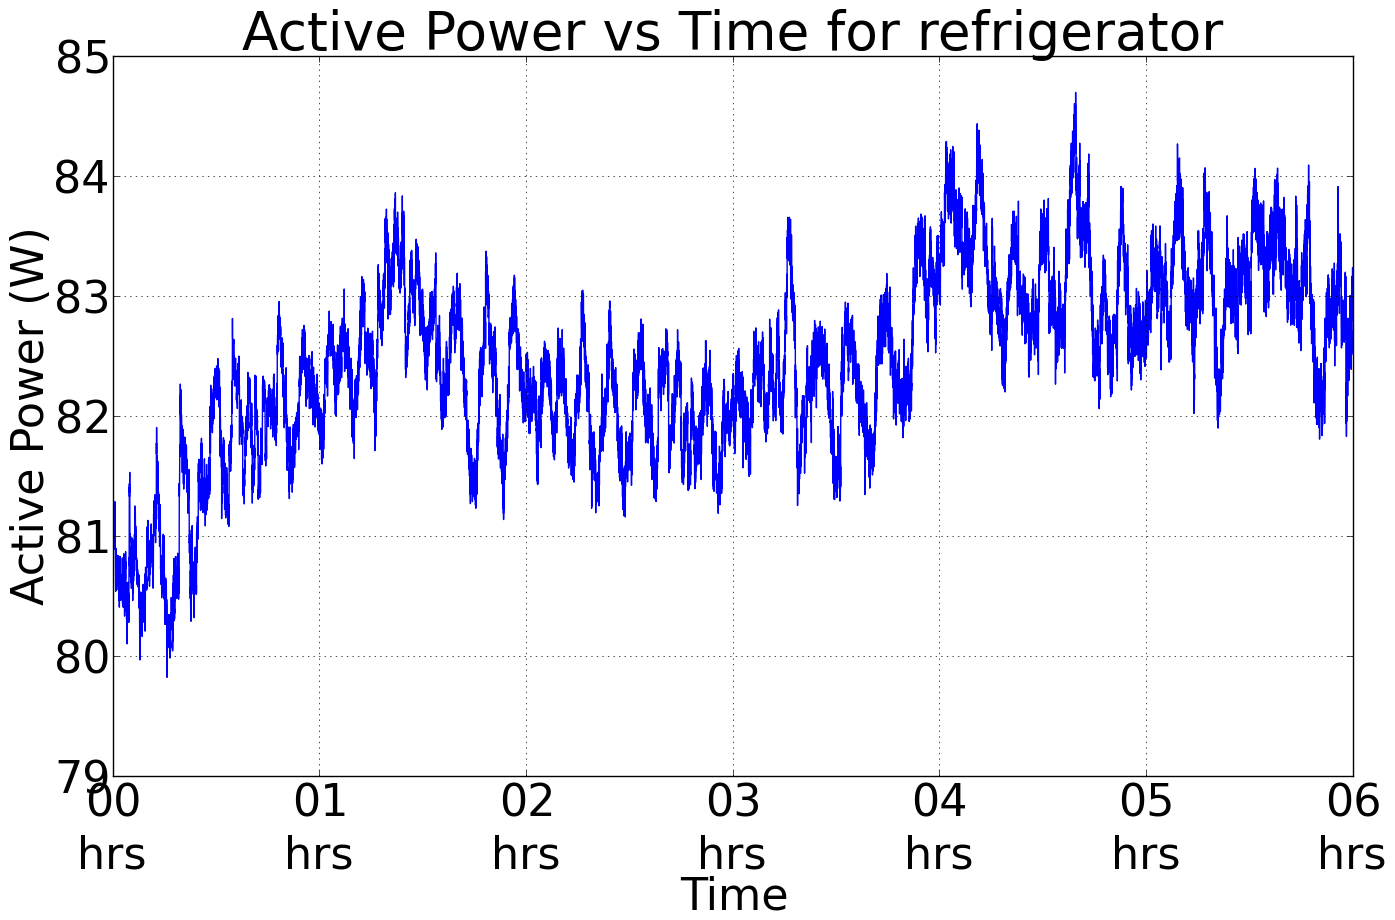
\includegraphics[scale=0.1]{./figures/after_repair.png}}
       
   \vspace{-3mm}
    \caption{Refrigerator power consumption}
    \label{fig:metadata}
    \vspace{-4mm}

\end{figure}
	
\noindent \textbf{Importance of meta data collection:} We collected metadata associated with electrical appliances throughout our deployment. We collected parameters such as appliance name, age, mode of usage (eg. air conditioner set temperature). We believe this detailed metadata can enhance NILM and can provide useful insights for conserving electricity. An anecdotal evidence illustrates the utility of meta data collection. The home refrigerator was repaired on 2$^{nd}$ July. \figref{fig:before_repair} and \figref{fig:after_repair} show the active power consumption before and after the repair. We observed that after repair, the refrigerator was set to the lowest temperature setting by the service professional, while before repair it was set to highest temperature setting. After the repair, the refrigerator was found to be consuming 1KWh more per day (which is 140\% above the normal). The residents configured their refrigerator again to the lowest temperature setting after we informed them about the increased energy usage, after which, its power consumption returned to previous levels. 
%Moreover, its duty cycle pattern was significantly modified. 
This metadata can be useful to NILM approaches modeling duration of appliance usage. 
% possible consider % % % % % % % % % % % % % % % % % % % % % % % % % % % % % % % % % % % % % % % % % % % % % % % % % % % % % % %
%
%\redcolor{To make the case even stronger, i am thinking of putting the need for measurement calibration for different h/w}
% % % % % % % % % % % % % % % % % % % % % % % % % % % % % % % % % % % % % % % % % % % % % % % % % % % % % % % % % % % % % % % % %
%\redcolor{Was this increased energy with higher setting or even after you reduced the setting?}

\noindent \textbf{Load specifics:} Appliance usage varies significantly in India compared to the USA and the Europe. Number of automated loads (e.g. dishwasher that work without any human intervention) is fewer and temperature control is often decentralized (i.e. a separate air conditioner at the room level and separate water heating, using a device commonly called as geyser, at the bathroom level). From our deployments, we observed that air conditioners and geysers account for up to 70\% and 50\% of the overall home electricity in summers and winters respectively. Thus, small improvements in efficiency of these two appliance can significantly lower the home electricity consumption. From NILM perspective, these loads are simple to disaggregate due to their high power consumption and repeated patterns (shown by the compressor in the air conditioner). Correspondingly, even a simple NILM approach can potentially provide useful insights towards energy reduction in the Indian context.

\noindent Additional energy is embedded into the water at the home level due to its low pressure and poor quality. Water pumping and filtering are the two activities whose scope spans across both water and electricity dimensions. Due to limited supply and line pressure, a water motor is used to pump the water up to the water tank on the roof. We observed that to fill 1 liter of water into the tank, it took 8 seconds without the motor (during the times of maximum pressure) and 4 seconds when the motor was used. With power consumption of 700 W for the electric motor, every one hour usage will result in additional energy being embedded into the water due to its intermittent supply. % was approx. 700 W. To fill an empty water tank (\redcolor{mention its capacity}) it would take 8000 seconds (2 hours 12 mins) without motor and 4000 seconds (1 hours 6 mins) with motor. An additional 770 Wh energy would be consumed if the motor is used. Thus, there is a fine balance between electricity consumption and time taken to fill the tank. We found that motor is typically used for 10 minutes in a day.
%Since water flow from utilities is provided only for about 1 hour each in the morning and evening, motor is used for about 10 minutes a day.
Due to poor quality of supplied water (and often the consumed water is the ground water and not the utility supplied water), Reverse Osmosis(RO) based water filters are commonplace in big cities in India. We observed that water filter takes approx. 1 minute to filter 1 liter of water and consumes 40 W in the process. 
%Thus, the water filter would consume 20 Wh energy for filtering 30 liters of water (typical drinking water usage).

\noindent Another interesting distinction in the Indian context is that each plug point has an associated switch and people are often conscious about turning the appliance off from the switch rather than keeping them in the standby (as is the usual practice in the USA). We observed that the jPlugs attached to the kitchen appliances such as microwave, when used for less than 1 minute, did not report data. This was due to the fact that jPlug takes roughly a minute to establish WiFi connectivity and then starts data collection, and before it could do so, the appliance was turned off.
% We also did a survey of more than 800 households in Delhi which reported that typical microwave and mixer usage was less than 2 minutes. \redcolor{Did you download the survey response and took this data from there?}. 
Correspondingly, \emph{building monitoring and control systems for the Indian context should account for the short appliance usage and power off from the switch to ensure robust and reliable data collection.}
%If the appliances were to be always on, this data would not have been lost. 
%From our survey with the home occupants, we found that their 
% We seek to resolve this issue in our future deployments.

\noindent \textbf{Lack of COTS devices made for Indian settings:} As reported earlier in \secref{sec:sensing}, due to non availability of ZWave sensors for Indian frequency, we imported European frequency based multisensors and plug load monitors. Import duty and shipment delays make them an expensive choice. Further, to avoid the peak switching current, the default state of the plug monitors was off (when powered manually from the switch). This implied that unless they are switched on from the software (or with a separate ZWave based switch), they will not turn on the appliance. Since many of the loads in the Indian context are not always on and are controlled via plug sockets, such plug sockets did not result in seamless usage. Correspondingly, we did not use ZWave based plug load monitors in our deployments as they had to be manually turned on after a power outage, which is common. %Also, solutions for panel level monitoring are not easily available in India.
% Further, other alternatives like Current Cost based CT's involve exposing live wire from appliances, an option which was rejected by home occupants. Also, Current Cost based Individual Appliance Monitors (IAM) provide only apparent power and energy at low frequency. 
Correspondingly, we had to resort to prototype solutions for appliance and circuit level monitoring.
\vspace{-1mm}
\section{Hitchhiker's guide revisited}
\label{sec:common}
While there are several unique observations from our deployment, there exists multiple similarities with prior deployment experiences, most specifically- ``The Hitchhiker's Guide to Successful Residential Sensing Deployments"~\cite{hitchhiker_residential}. Some prominent similarities are:

\noindent \textbf{Homes are hazardous environments:} We observed that one of our multisensors would fail after power outage. %Initially, we felt that the sensor was faulty, but other multisensors also showed the same behavior in the same location. 
We, eventually, figured that this behavior was due to the fact that this multisensor was put on the inverter point (battery backup, as is common in many homes to guard against intermittent power supply) and would not fail during a power outage. Thus, when the main power resumed, ZWave controller was not able to add this multisensor to its network. We resolved this by putting the multisensor at a non-inverter point. We also observed that one of the multisensor would always indicate motion. Initially we solved this problem by replacing its power supply. However, within a week, this problem resurfaced. We believe it is due to the faulty power supply in that room. The home occupants did not allow a thorough investigation of that electrical socket and we had to do away with that data.
Although we used zip-ties extensively throughout the deployment to prevent hanging wires, we observed data loss in one of our multisensor and Android phone, which went out of power due to wire snag (shown in \figref{fig:snag}). Even after one month rigorous testing in the lab, before we started the deployment, we raised 60 new service complaints, when we moved the deployment to this home. This is a testimony that homes present unique challenges which can not be exactly emulated in laboratory settings.

\noindent \textbf{Aesthetics matter:} As stated in the previous work, sensor LEDs can be bothersome to home occupants, particularly in the night. Our 33 sensor deployment had introduced 63 LEDs in the home. \figref{fig:led} shows our sensor LEDs blinking in the night. Choosing appropriate sensor location sufficed for our present deployment. However, for future such deployments, we intend to build better sensor casing to ensure that home occupants are not disturbed. Also, the home occupants complained of buzz like sound coming from the desktop that we had installed. This noise was due to the dust clogging in the desktop. Dust is a uniquely common aspect in the Indian setting. Correspondingly, {monitoring and control systems, aiming for long life deployments should include routine maintenance, to guard against dust and other environmental problems.}

\noindent \textbf{Homes are not designed for sensing:} We observed that the data collected from our ground floor MCBs (5 in number) was noisy. This was due to the fact that these MCBs are close (shown in \figref{fig:ct_interference}) to each other causing interference in our CT monitoring circuit. A workaround could have been to get additional cabling done, but the residents were not inclined for such changes. For the 3 MCBs on the first floor, there was adequate gap amongst them and the data was of good quality (verified using manual experiments involving switching appliances on those circuits). %We, thus, believe that homes are not designed for sensing and one may not be able to sense desired parameters.

\noindent \textbf{Redundancy-Accounting for sensor failure:} During our deployment 3 jPlugs and 1 multisensor stopped functioning properly. We had accounted for such failure and had kept reserve sensors ready. %We believe that one should beforehand account for sensor failure in residential deployments.

\noindent \textbf{Homes have poor connectivity:} During the preliminary phase of our deployment, we first tried to connect our sensors to the existing networking infrastructure in the home. Already existing WiFi router was on the first floor and we observed poor signal strength on the ground and the second floor. We used Ekahau Heat Mapper\footnote{\url{www.ekahau.com/products/heatmapper/overview.html}} to map WiFi signal strength. \figref{fig:ground_without_router} and \figref{fig:second_without_router} show the WiFi heatmap produced with the home router placed on the first floor. We observed that a lot of regions inside the home show poor signal strength. We bridged an additional router on the ground and the second floor with the existing first floor router. \figref{fig:ground_with_router} and \figref{fig:second_with_router} show the corresponding WiFi heatmaps produced after the introduction of bridged routers. Additional routers significantly improved WiFi coverage. 

%\noindent Another important facet of deployments is that additional sensors introduced inside a home may choke up the network bandwidth. We observed this when we tried using imported WiFi based microcontrollers for sensing ambient conditions in our research wing. Research wing occupants complained of low network bandwidth available for their personal usage. Thus, we decided to use ZWave based multisensors for measuring ambient parameters for home deployment. Since ZWave based sensors worked on a different frequency (868.4 MHz) as WiFi(2.4 GHz), they did not cause interference. We believe that a careful mix of sensors working on different frequencies can be used to avoid interference issues.
\begin{table}
\tabcolsep=0.015cm
\vspace{-4mm}
\caption{First floor water fixtures labeled metadata}
\vspace{-4mm}
\label{tab:water_consumption_labeled}
\footnotesize
\begin{tabular}{|c|c|c|c|c|}
\hline
\textbf{Sno.}&\textbf{Type}&\textbf{Consumption}&\textbf{Purpose}&\textbf{Location}\\
\hline
1&Flush&10 liters per flush; 210&Toilet&Bathroom\\
 &&seconds for flush tank to refill&flushing&cum toilet\\ \hline
2&Tap&17.5 l/minute&Washing clothes&Washing area\\ \hline
3&Tap&5 l/minute&Washing hands&Washbasin\\ \hline
4&Tap&7 l/minute&Bathing&Bathroom\\ \hline
5&Tap&1 l/minute&Bathroom cleaning&Bathroom\\ \hline
6&Tap&13.2 l/minute&Gardening&Veranda\\ \hline

\end{tabular}
\vspace{-6mm}
\end{table}
\begin{figure}[t!]  
\vspace{-2mm}
\subfloat[\scriptsize Ground floor WiFi Heatmap without additional router]{
	 \label{fig:ground_without_router}
    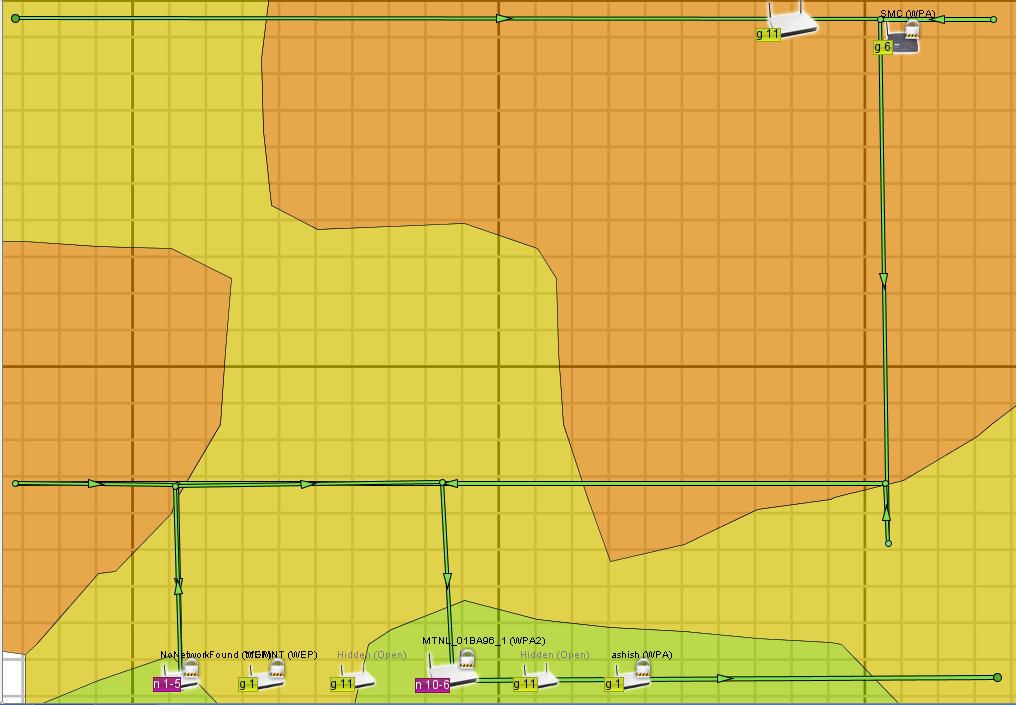
\includegraphics[scale=0.05]{./figures/ground_without_router.png}}
    \hspace{0.4mm}
    \subfloat[\scriptsize Ground floor WiFi Heatmap with additional router]{
    	 \label{fig:ground_with_router}
        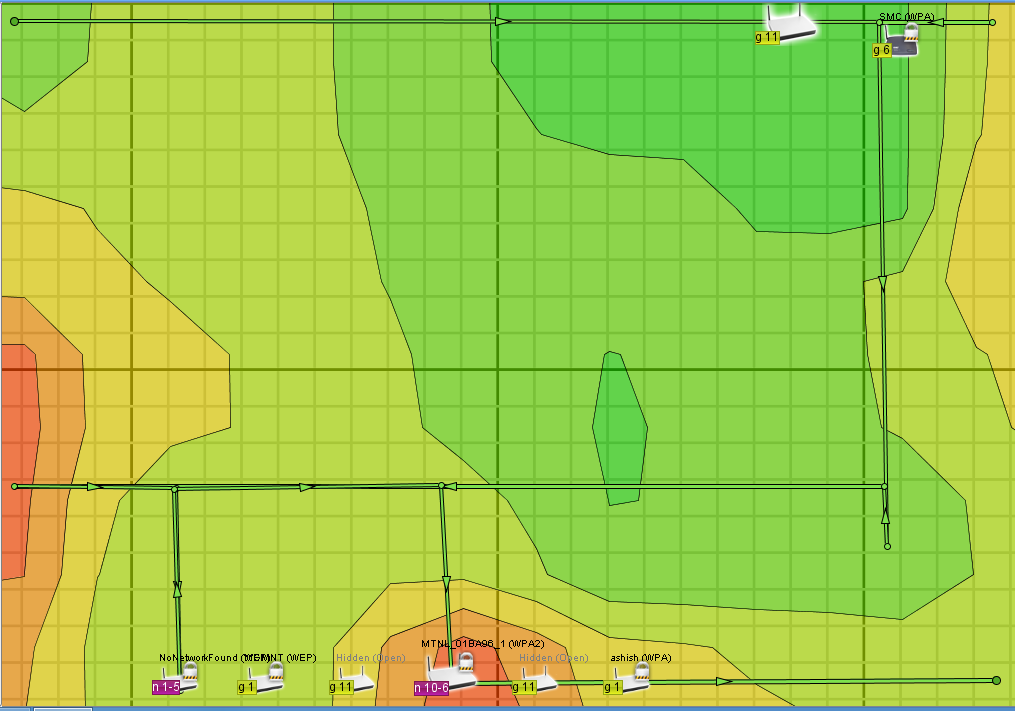
\includegraphics[scale=0.05]{./figures/ground_with_router.png}}
%       \subfloat[]{
%       	 \label{fig:heatmap}
%           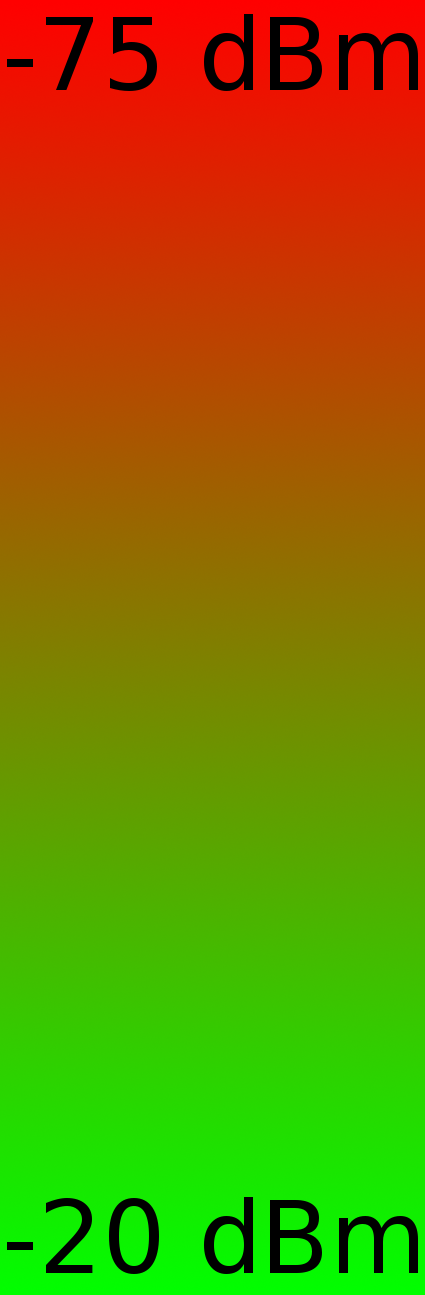
\includegraphics[scale=0.1]{./figures/heatmap.png}}
%        \vspace{-3.5mm}
%       \newline
\hspace{0.4mm}
      \subfloat[\scriptsize Second floor WiFi Heatmap without additional router]{
      	 \label{fig:second_without_router}
          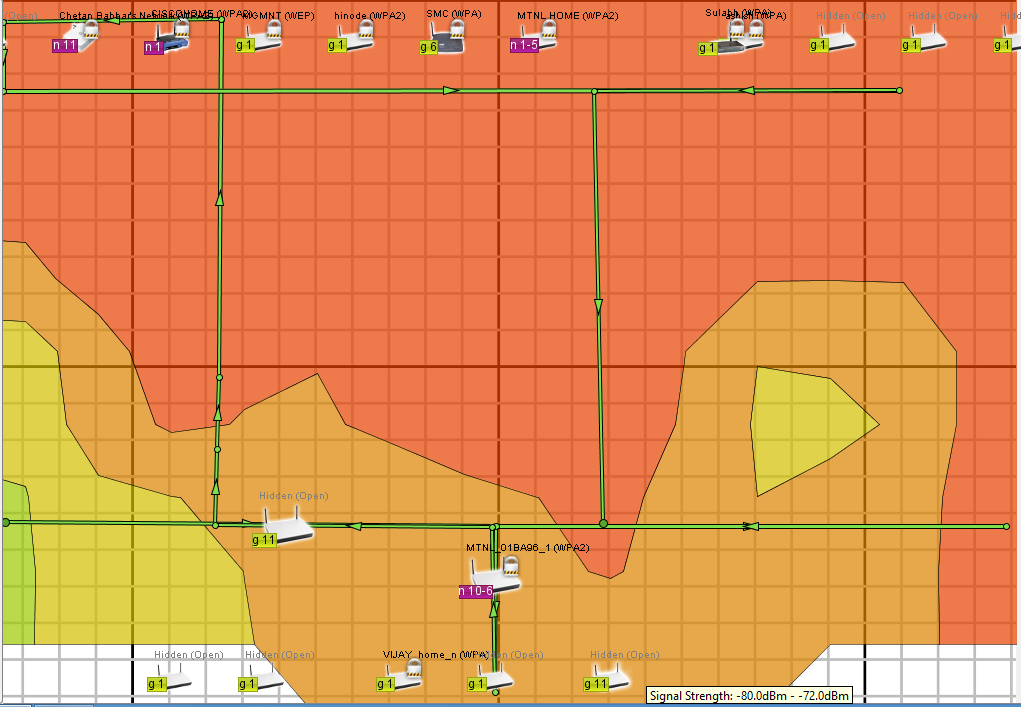
\includegraphics[scale=0.05]{./figures/without_.png}}
          \hspace{0.4mm}
          \subfloat[\scriptsize Second floor WiFi Heatmap with additional router]{
          	 \label{fig:second_with_router}
              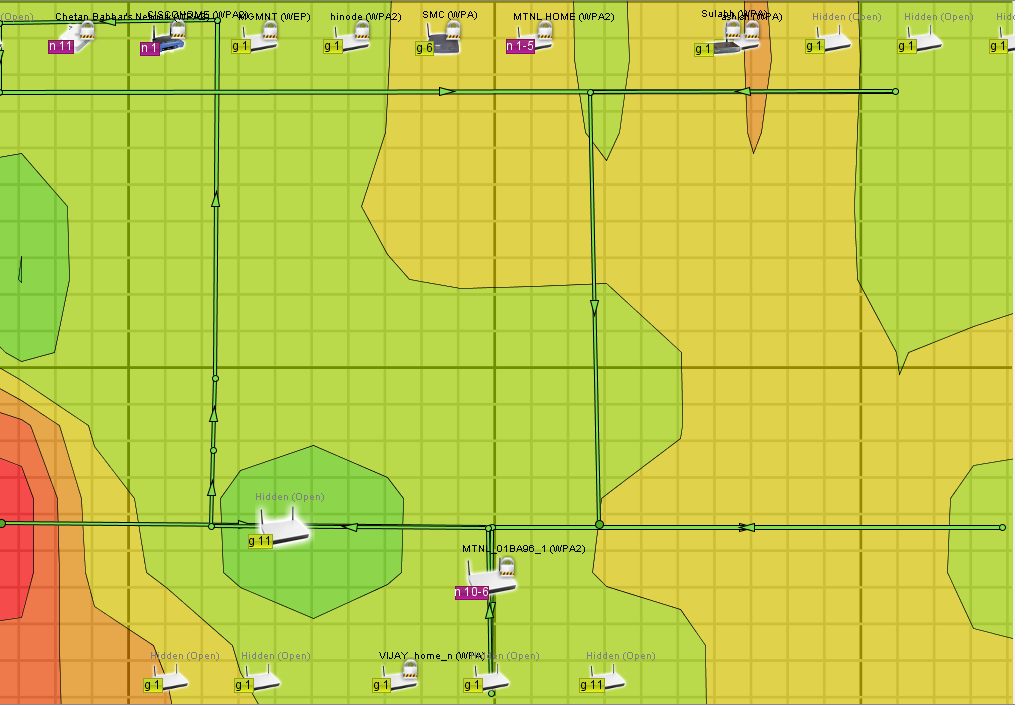
\includegraphics[scale=0.05]{./figures/with_.png}} 
              \hspace{0.4mm}
              \subfloat[\scriptsize Scale]{
                     	 \label{fig:heatmap}
                         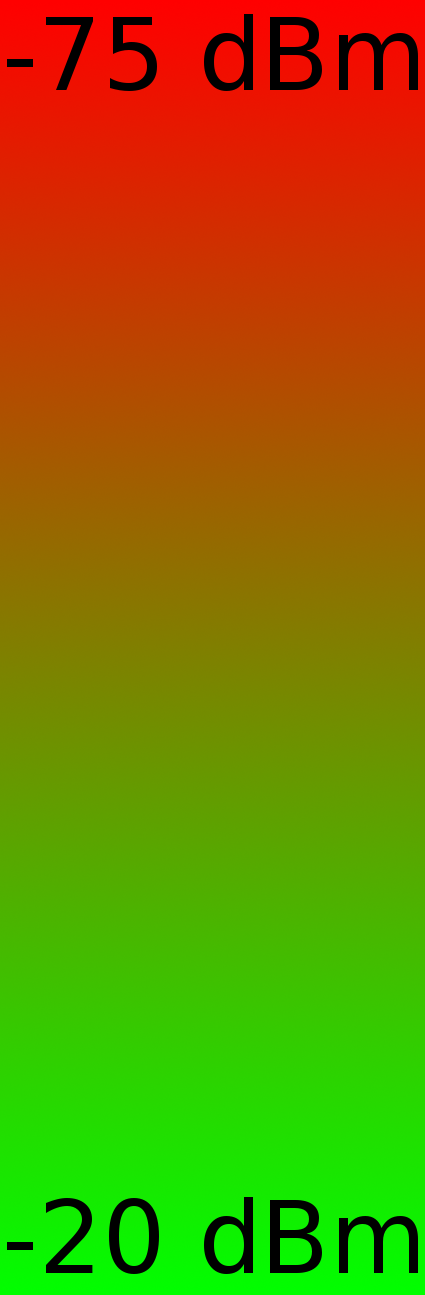
\includegraphics[scale=0.0275]{./figures/heatmap.png}}
              \vspace{-3mm}
    \caption{WiFi signal without placing additional routers on different floors is poor. The greener the region, the better the signal strength for the heatmap. 
%    \redcolor{Show the scale for the heatmap on the side as well.}
}
\end{figure}








\begin{figure}     
    \subfloat[\scriptsize Glowing LEDs in night]{
        \label{fig:led}
        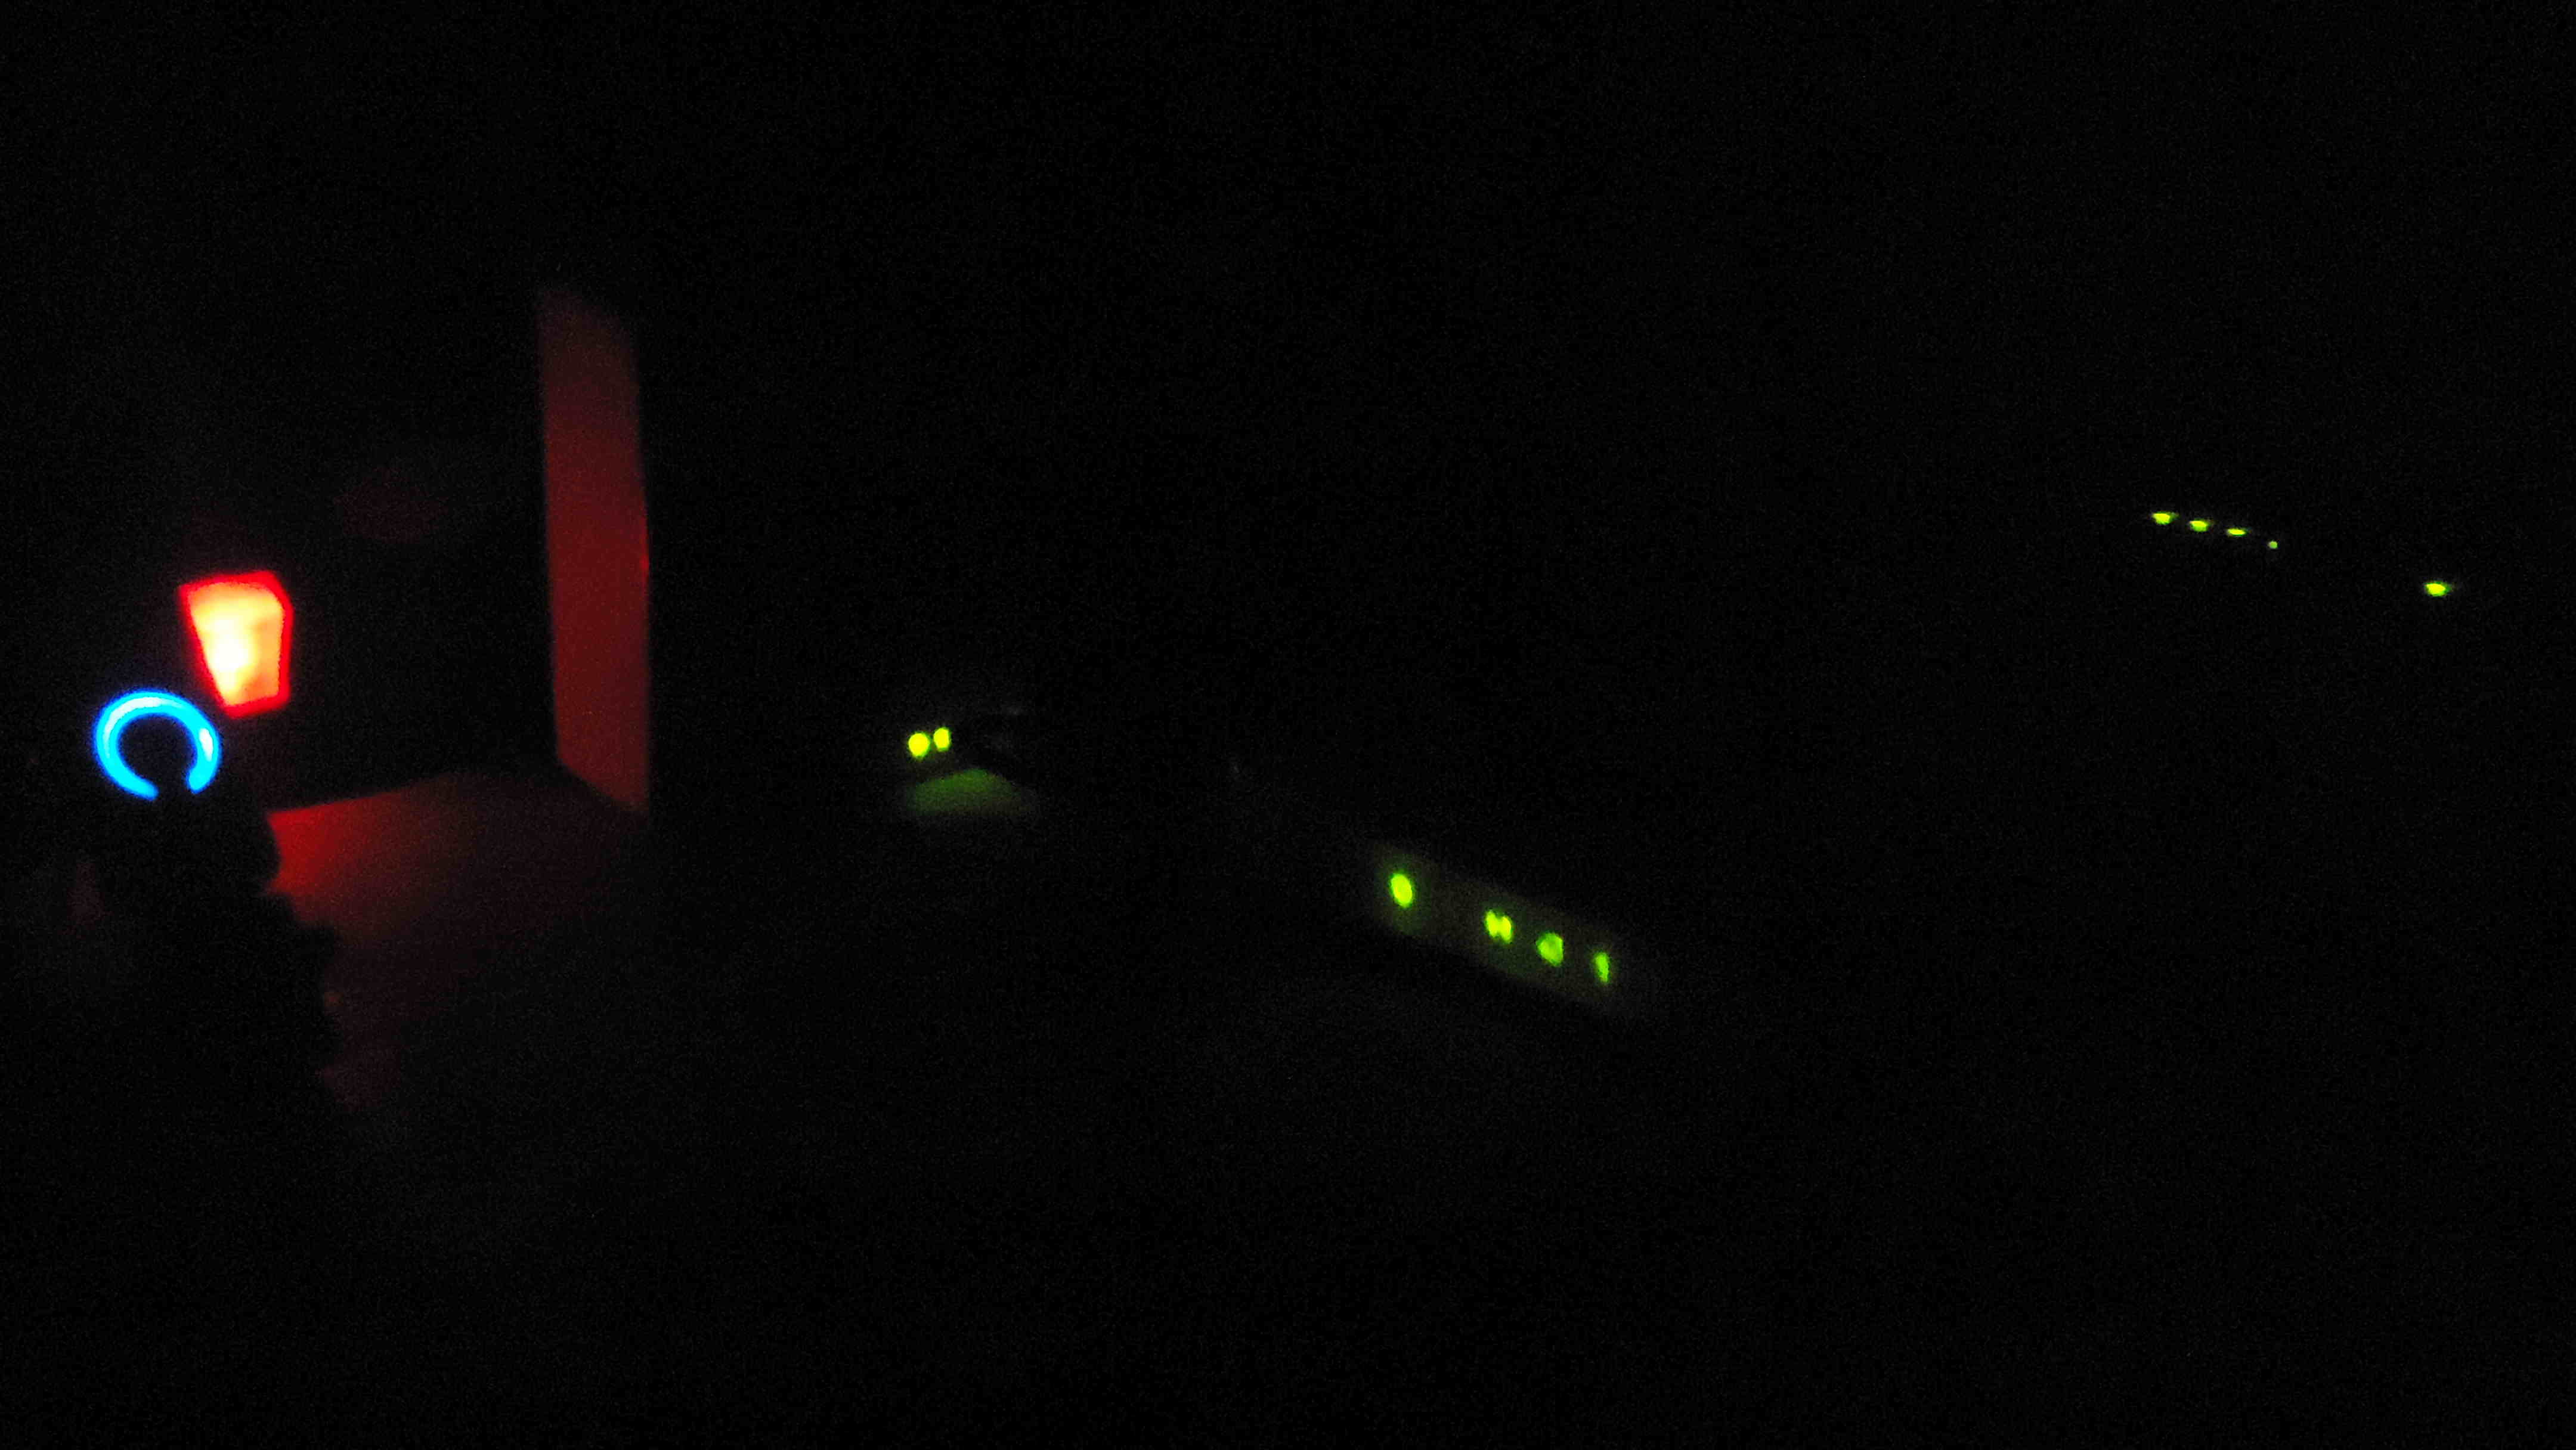
\includegraphics[scale=0.017]{./figures/led.jpg}}
        \hspace{0.02mm}
         \subfloat[\scriptsize Wire snag leading to data loss ]{
            \label{fig:snag}
            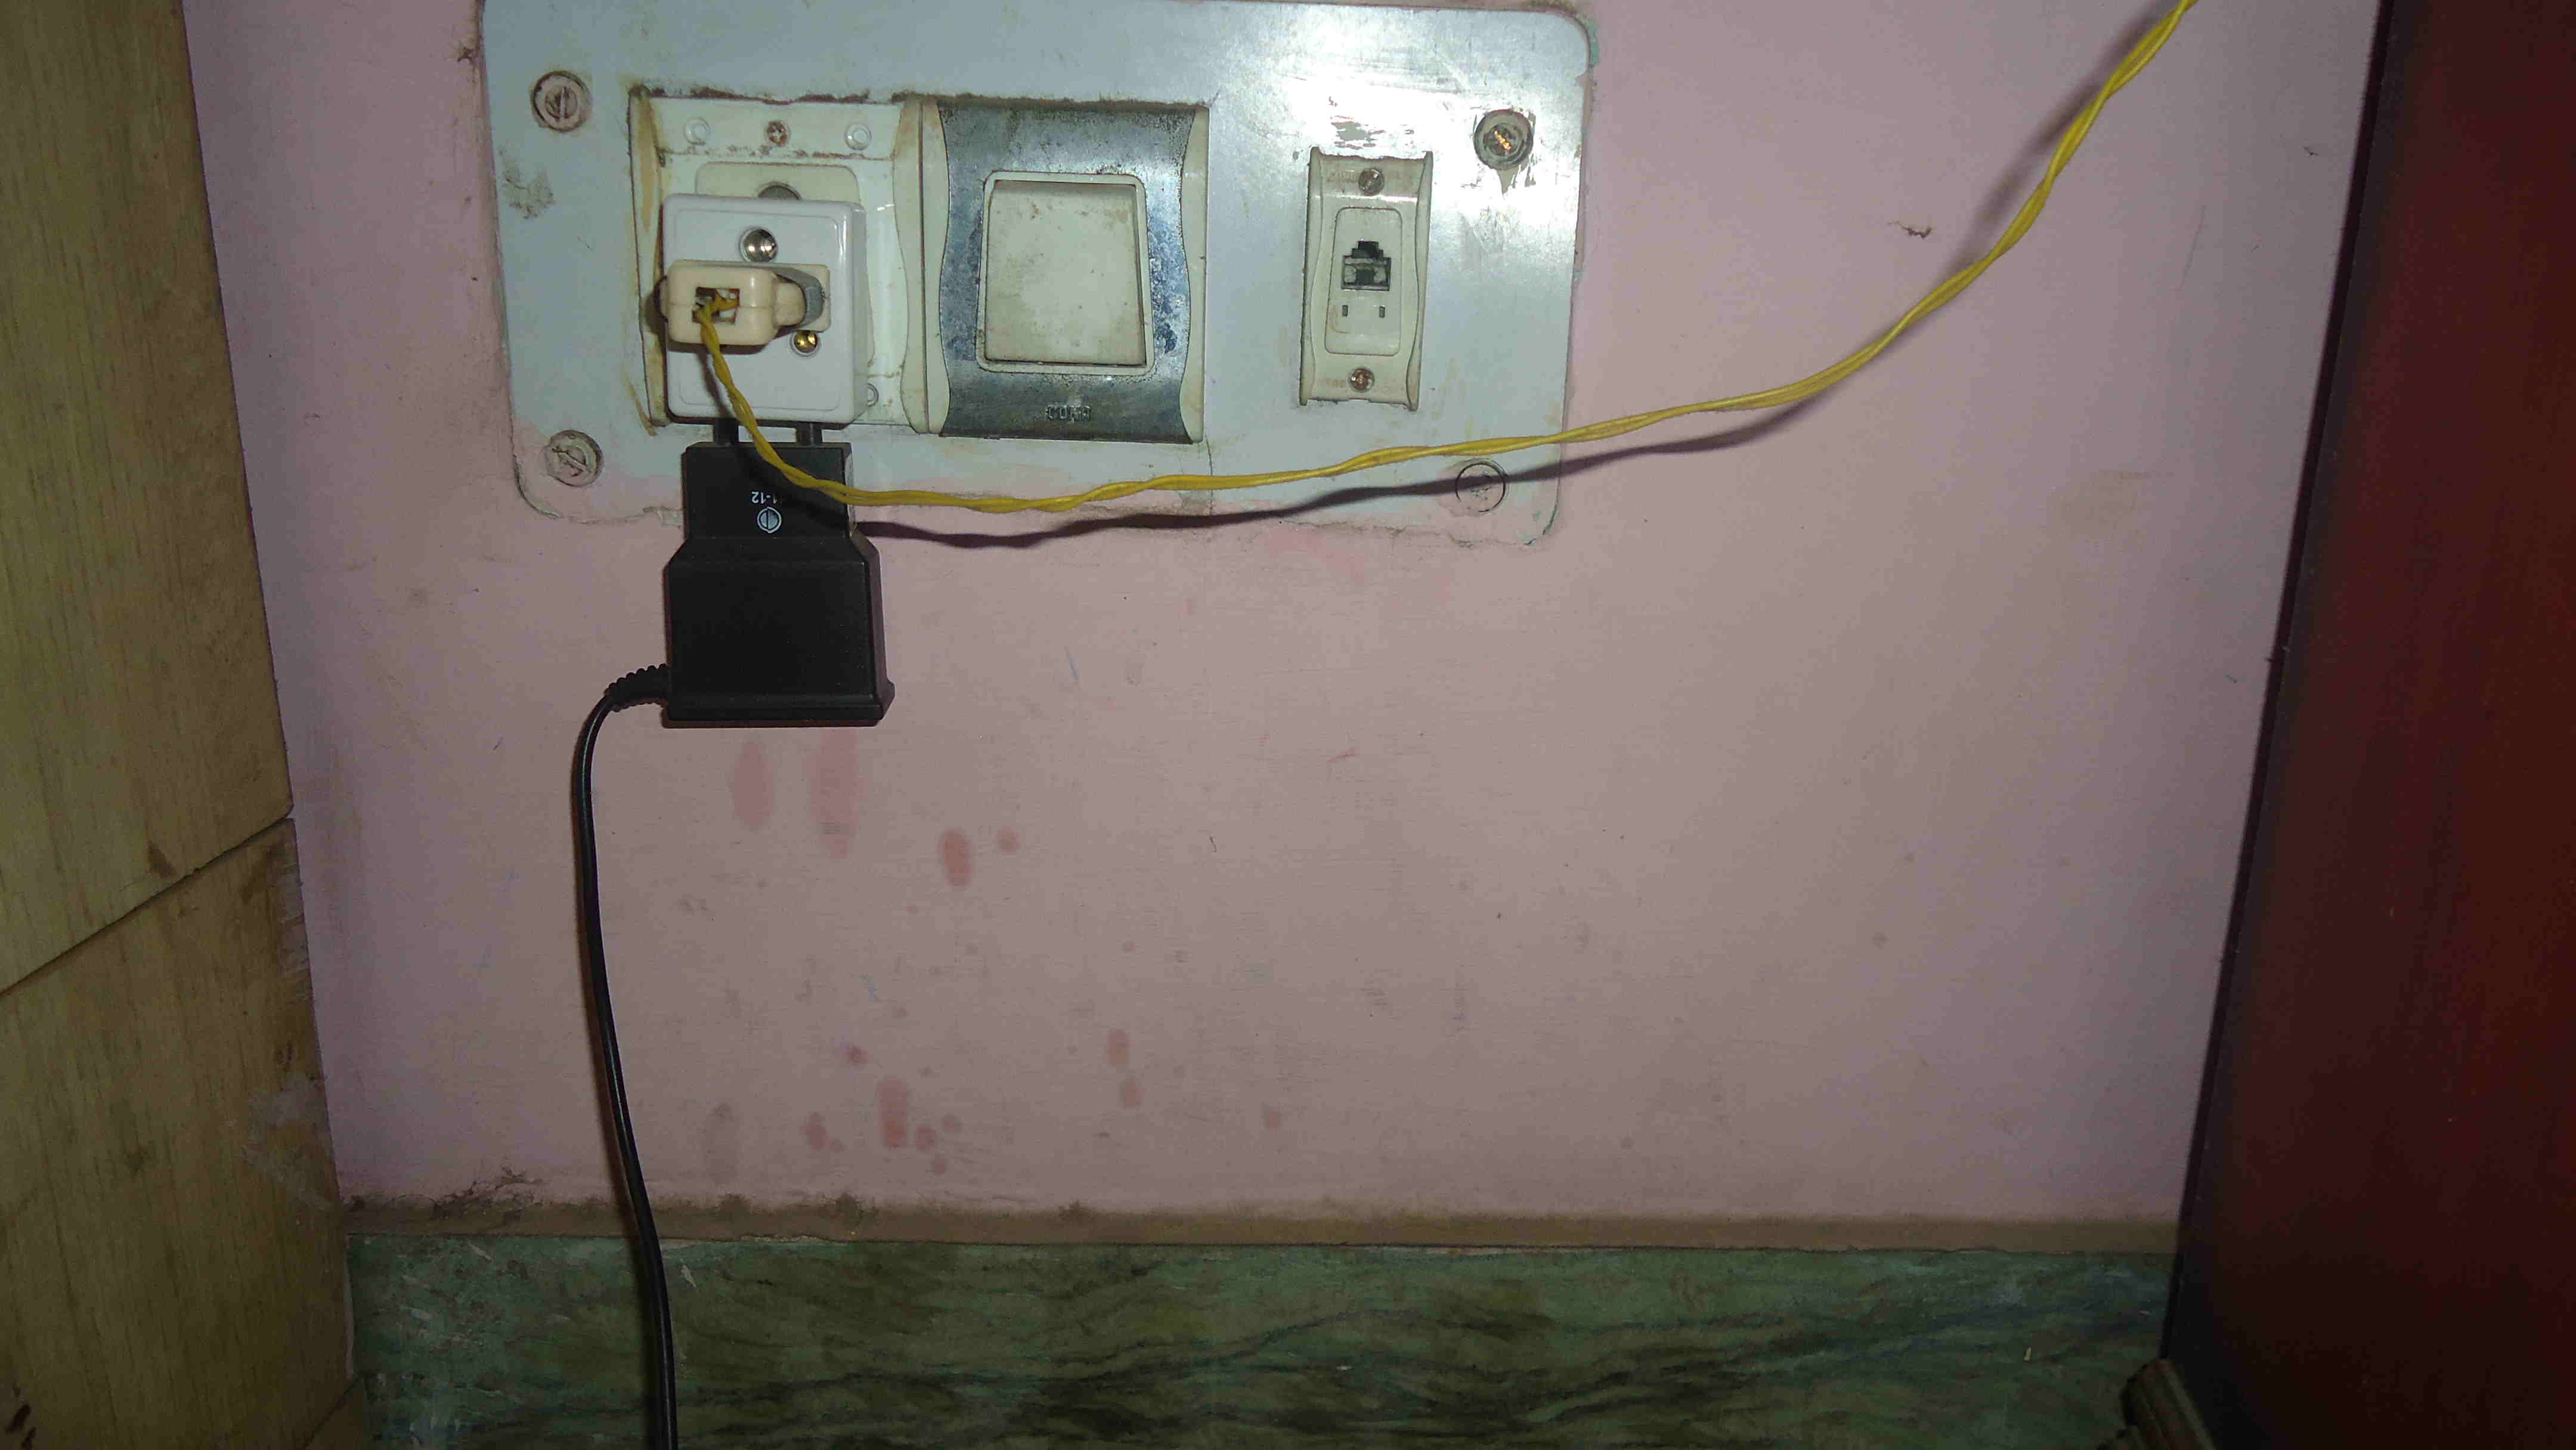
\includegraphics[scale=0.017]{./figures/snag.jpg}}
                    \hspace{0.02mm}
        \subfloat[\scriptsize Closely placed MCBs causing interference in CT monitoring circuit ]{
                    \label{fig:ct_interference}
                    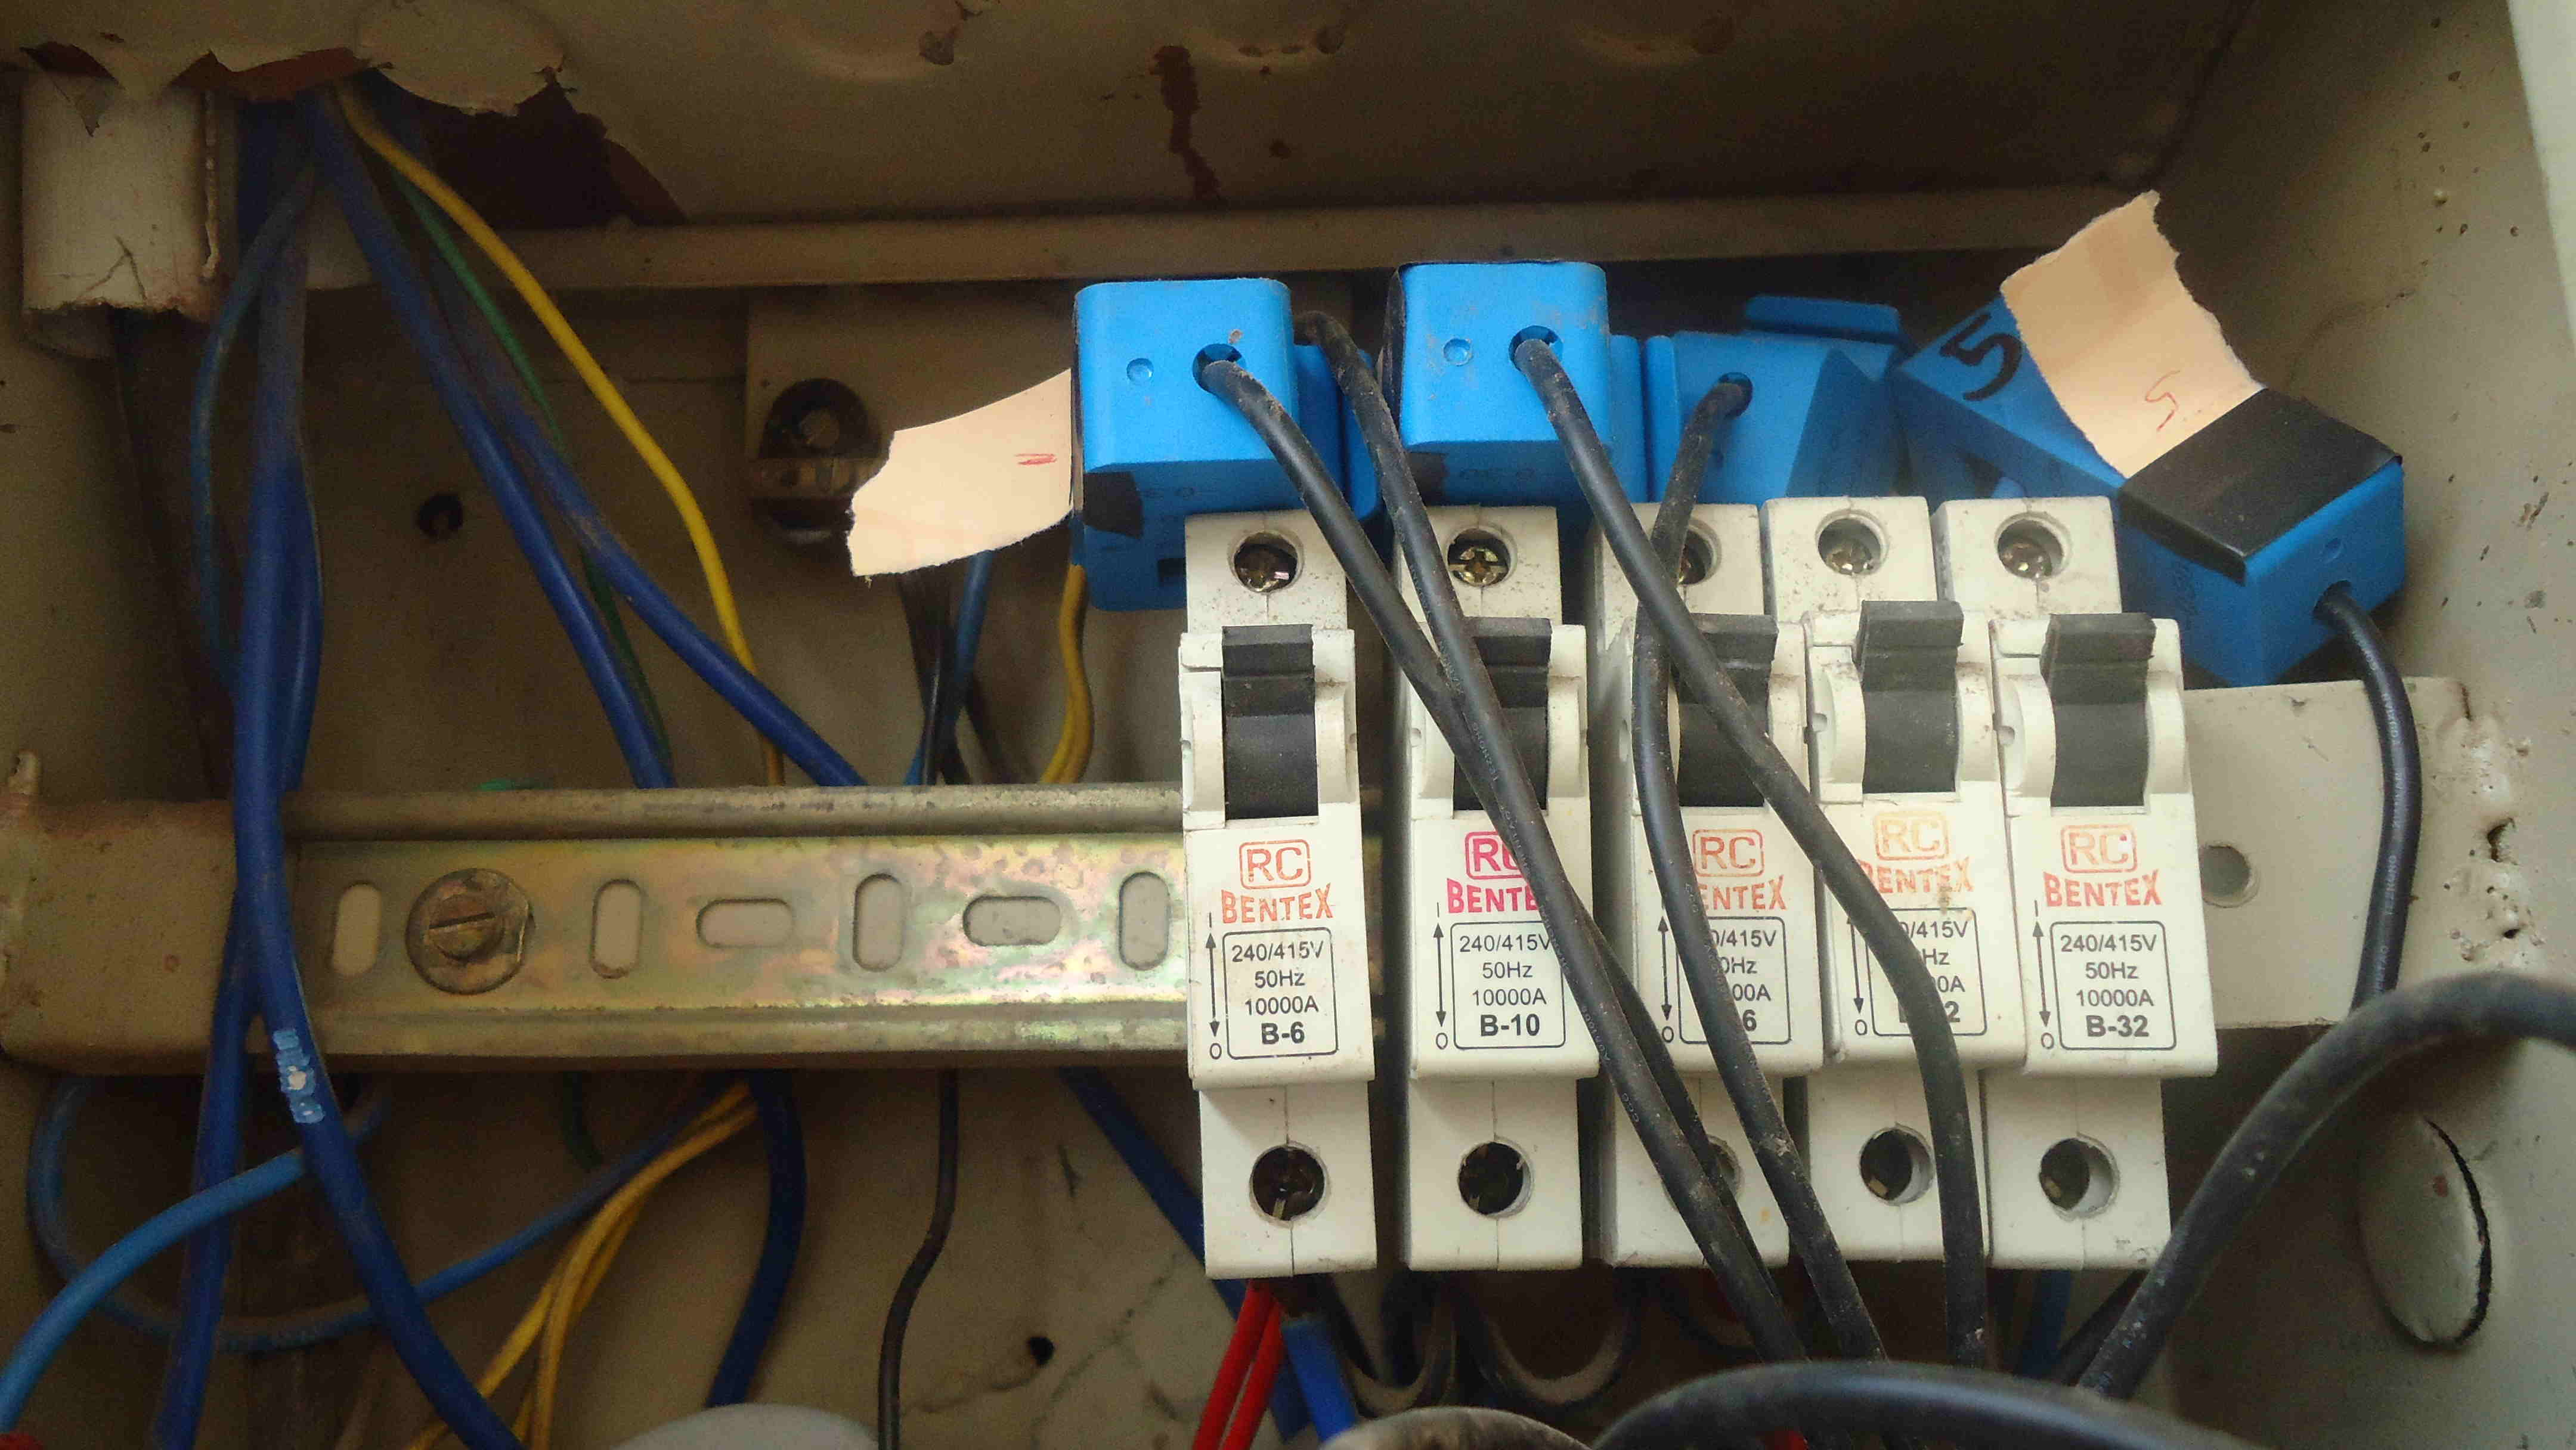
\includegraphics[scale=0.017]{./figures/ct_interference.jpg}}
                    \vspace{-3mm}
    \caption{Common problems in residential deployments}   
    \label{fig:home}
   \vspace{-3mm}
\end{figure}
\vspace{-1mm}
\section{Dataset and code release}
Inspired by previous work~\cite{blued_cmu}, we release fully labeled data for 1 day. This dataset is of the first of it's kind, across the world, where events corresponding to electricity, water and ambient sensors are timestamp recorded. We manually annotate the power consumed for each of the x appliances in their different states in the home. We similarly measure the amount of water consumed in 1 minute by each of the y water fixtures. \tabref{tab:water_consumption_labeled} shows the consumption pattern of water fixtures on the first floor. We further provide a detailed metadata log of all electrical appliances, including, but not limited to, estimate date of purchase, mapping to MCB, star-rating, rated power. We intend to release more such fully labeled data in the future, but owing to privacy concerns, we limit the current fully labeled dataset to 1 day from this home. While the accompanying switch had been to our disadvantage in measuring short duration appliance usage, it provides us an advantage over the data collected in developed countries setting. By virtue of switch control, atleast the ON-OFF events can be clearly demarcated. Thus, in some sense, our entire electrical dataset is event labeled. 

\begin{figure} 
	\vspace{-5mm}    
    \centering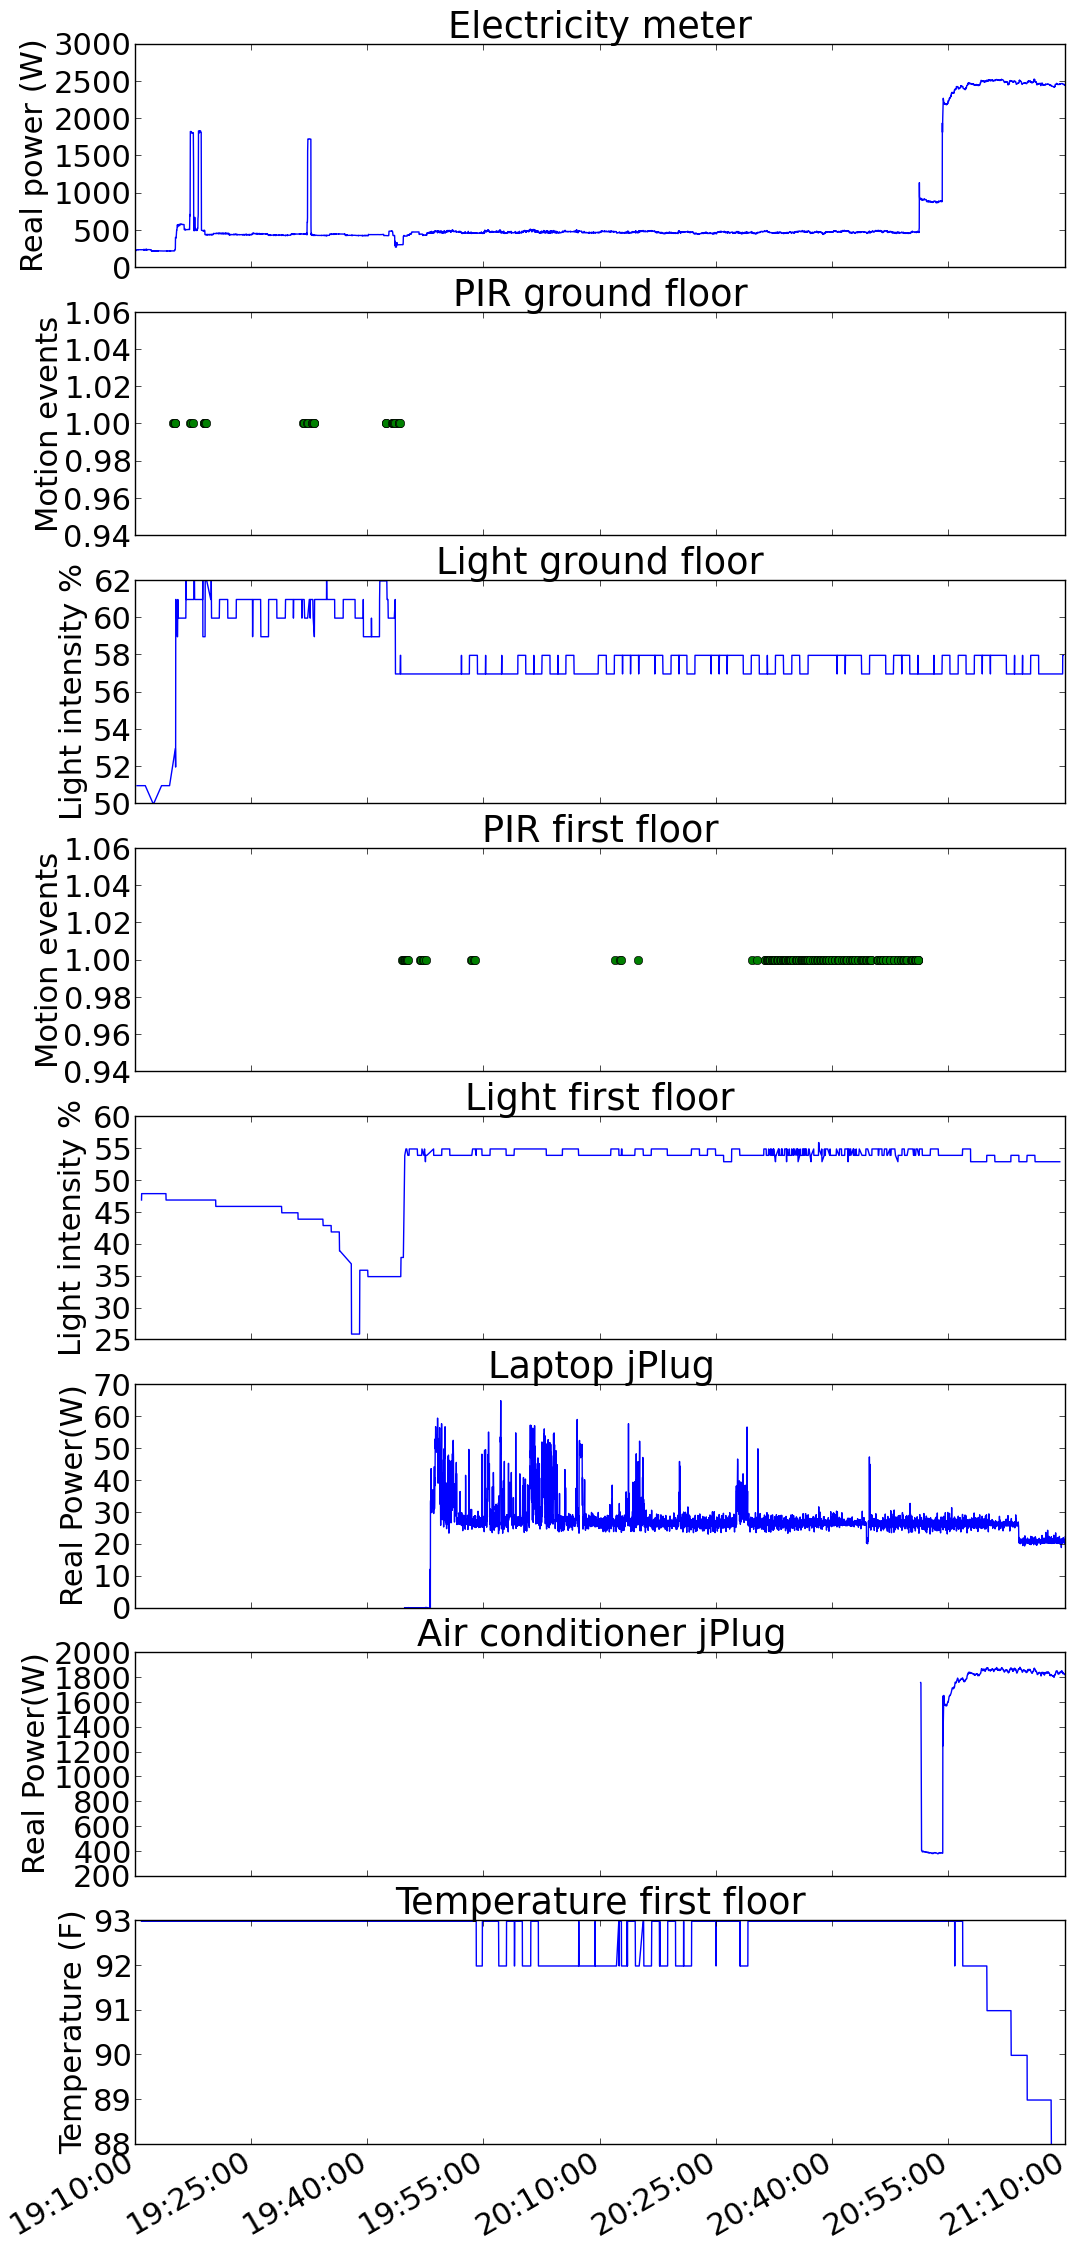
\includegraphics[scale=0.19]{./figures/label.png}
	\vspace{-2mm}    
    \caption{Labeled dataset} 
%    \vspace{-2mm}  
    \label{fig:labeled}
\end{figure}

\looseness -1 We publicly release our codebase which includes \selstups implementation, scripts for collecting data from different sensors, database schemas, soft-sensors, startup scripts and the fixes we developed for common problems on RPi. Our codebase and dataset\footnote{\url{http://github.com/nipunreddevil/Home_Deployment}} can be found on Github.

\noindent 

\vspace{-1mm}
\section{Conclusions and Future Work}
\looseness -1 In this paper, we present our experiences with an extensive residential deployment monitoring electrical, water and ambient parameters in Delhi, India. To the best of our knowledge, this is the first extensive residential deployment in a developing country. We present key aspects of our deployment and discuss the corresponding impact on the design of building monitoring and control systems that aim to scale across diverse contexts offered in the developing and the developed countries. Some of the unique aspects, impacting the systems development in building energy domain, include - unreliable electrical grid, unreliable network connectivity, differences in electrical loads, water-embedded energy within a home and limited availability of robust COTS infrastructure. We further discussed the similarities in our learning with prior work (done in the USA), demystifying the home environment for energy and water related deployments in the Indian context. %importance of poor wireless connectivity in homes and the importance of aesthetics.

Frequent power outages and unreliable internet motivated us to develop the proposed sensing architecture: \selstup, which accounts for these pitfalls by introducing local storage and periodic upload. Such an architecture can be of particular importance in the context of building monitoring and control systems suitable for the developing countries. 

We are in the process of installing our sensors across multiple other homes in Delhi. Data from the deployment will be released for public use after necessary post processing and filtering, to ensure privacy and appropriate usage. We further plan to carry out longer duration deployments capturing seasonal variations in energy usage patterns. %and after that we wish to release our data set in the public. 
%We are also developing a billing application for providing detailed electricity usage information to home owners. 
%We plan to perform NILM and provide the home occupants with detailed electricity consumption breakdown.

\balance
\vspace{-1mm}
\bibliographystyle{abbrv}
\bibliography{references} 

\end{document}
